%http://texblog.org/2011/09/09/10-ways-to-customize-tocloflot/

%Автоматически вписывать картинки в ширину страницы:
%\includegraphics[maxwidth=\linewidth]{foobar}

\if 0
Так можно сделать многострочный комментарий.
Это маленький хак. Его надо использовать.
\fi

\documentclass[twoside,11pt,a4paper,notitlepage]{report}

\makeatletter
\newcommand*{\toccontents}{\@starttoc{toc}}
\usepackage{pscyr}
\usepackage[T2A]{fontenc}
\usepackage[utf8]{inputenc}
\renewcommand{\rmdefault}{CMR}
\usepackage[russian]{babel}
\usepackage[dvipsnames]{xcolor}

%\usepackage{classicthesis}
%\usepackage[toctitles]{titlesec}
\usepackage{listings}

\usepackage{titlesec}



% Создание индекса
%\usepackage{makeidx}
%\makeindex

%История изменений
%\usepackage{vhistory}
\usepackage[owncaptions]{vhistory}%[tocentry] включить в оглавление


\usepackage[most]{tcolorbox} % для управления цветом
\definecolor{block-gray}{gray}{0.90} % уровень прозрачности (1 - максимум)
\newtcolorbox{myquote}{colback=block-gray,grow to right by=-10mm,grow to left by=-10mm,
	boxrule=0pt,boxsep=0pt,breakable} % настройки области с изменённым фоном

%*************************
\usepackage{shorttoc}% Краткое оглавление
%*************************

%*************************
\usepackage{tocloft}% Управление оглавлением
%*************************



%Fncychar позволит выбрать несколько различных стилей, красиво оформляющих наименование глав.
%\usepackage[Glenn]{fncychap} % выбираем стиль Glenn

%Пакет titlesec позволяет вносить изменения в стандартный стиль главы, то есть переопределять его.
%\usepackage{titlesec, blindtext, color} % подключаем нужные пакеты
%\definecolor{gray75}{gray}{0.75} % определяем цвет
%\newcommand{\hsp}{\hspace{20pt}} % длина линии в 20pt
%% titleformat определяет стиль
%\titleformat{\chapter}[hang]{\Huge\bfseries}{\thechapter\hsp\textcolor{gray75}{|}\hsp}{0pt}{\Huge\bfseries}

\usepackage{listings}      % для кусков программ 
% (понимает синтаксис некоторых языков, чума просто)
\usepackage{alltt}         % для того же
\usepackage{amssymb}       % прикольно для формул

\pagestyle{plain} % нумерация страниц вкл.

%http://tex.stackexchange.com/questions/181183/combine-usepackagetimes-and-fontspec-setmainfont
%http://andreyolegovich.ru/PC/LaTeX.php#base

%********************
% Набор предоставляет дополнительные математические символы, множество удобных возможностей для оформления математических формул (например, упрощённую работу с многострочными формулами) и используется почти во всех LaTeX-документах, в которых есть сколько-нибудь сложные формулы.
%******************** 
\usepackage{amsmath}



\usepackage{titlesec}
\usepackage{csquotes} % ещё одна штука для цитат

\usepackage{sectsty}
%\subsectionfont{\Large\underline}
\subsectionfont{\Large}

\usepackage{graphicx}
\usepackage{sidecap}
\usepackage{xcolor}
\usepackage{pdfpages}
\usepackage{comment}
\usepackage{textcomp}
\usepackage{wrapfig}
\usepackage{sectsty}
\usepackage{lipsum}
\usepackage{fancyhdr}
\usepackage{datetime}
\chapterfont{\centering}

\usepackage{caption}
\usepackage{subcaption}

\usepackage[T2A]{fontenc}
\usepackage{lscape}
\usepackage{makecell}
\usepackage{multicol}
\usepackage{floatrow}
\usepackage{float}
\usepackage{caption}
\usepackage{lastpage} % Allows referencing of the last page to allow footer to read: "Page [Current page] of [Total number of pages]."

\renewcommand{\familydefault}{\sfdefault} %Изменит стандартный шрифт документа на сансерифный.

\definecolor{MSBlue}{rgb}{.204,.353,.541}
\definecolor{MSLightBlue}{rgb}{.31,.506,.741}
%\titleformat*{\section}{\Large\bfseries\sffamily\color{MSBlue}}
%\titleformat*{\subsection}{\large\bfseries\sffamily\color{MSLightBlue}}
%\titleformat*{\subsubsection}{\itshape\subsubsectionfont}

\titleformat
{\chapter} % command
[display] % shape
{\bfseries\Large\itshape} % format
{Story No. \ \thechapter} % label
{0.5ex} % sep
{
	\rule{\textwidth}{1pt}
	\vspace{1ex}
	\centering
} % before-code
[
\vspace{-0.5ex}%
\rule{\textwidth}{0.3pt}
] % after-code


\titleformat{\section}[wrap]
{\normalfont\bfseries}
{\thesection.}{0.5em}{}

\titlespacing{\section}{12pc}{1.5ex plus .1ex minus .2ex}{1pc}





%*****************************************************
% Часто требуется, чтобы номер рисунка содержал в себе номер главы (вроде Рис. 1.1). Чтобы была сделана нумерация по главам, достаточно изменить счётчик рисунков в преамбуле документа вот так:
\renewcommand{\thefigure}{\thesection.\arabic{figure}}
%*****************************************************

%*****************************************************
%Если вас не устраивает вид подрисуночной подписи (например, вместо "Рис. 1:" необходимо "Рис. 1 --- "), используйте пакет caption. В частности, для установки тире в качестве разделителя, вставьте в преамбулу документа следующий код: 
\RequirePackage{caption}
\DeclareCaptionLabelSeparator{defffis}{ --- }
\captionsetup{justification=centering,labelsep=defffis}
%*****************************************************

%\usepackage[colorlinks=true,linkcolor=blue]{hyperref}

%*****************************************************
%Как сделать, чтобы уравнения нумеровались независимо по главам в LaTeX?
%В преамбуле
\makeatletter \@addtoreset{equation}{section} \makeatother 
\makeatletter \@addtoreset{figure}{section} \makeatother 
%*****************************************************

\addto\captionsrussian{
	\def\figurename{Рисунок}
}


\usepackage[hypcap]{caption}

%*****************************************************
% Начинать секции с новой страницы
\usepackage{titlesec}
\newcommand{\sectionbreak}{\clearpage}
%*****************************************************


%*****************************************************
%Чтобы в генерированном PDF работали гиперссылки, то надо подключить модуль hyperref (и если хотите их разрисовать, то модуль по работе с цветами xcolor):
\usepackage{hyperref}
% Цвета для гиперссылок
\definecolor{linkcolor}{HTML}{012b37} % цвет ссылок
\definecolor{urlcolor}{HTML}{012b37} % цвет гиперссылок
\hypersetup{pdfstartview=FitH,  linkcolor=linkcolor,urlcolor=urlcolor, colorlinks=true}
%*****************************************************

%***************************************************** 
%Для удаления номеров страниц из \listoffigures
\makeatletter
\newcommand{\emptypage}[1]{%
	\cleardoublepage
	\begingroup
	\let\ps@plain\ps@empty
	\pagestyle{empty}
	#1
	\cleardoublepage}
\makeatletter
%*****************************************************


\setcounter{secnumdepth}{3}
%\usepackage{enumitem}
\usepackage[shortlabels]{enumitem}
\setlist[enumerate]{leftmargin=*,align=left,label=\thesubsection.\arabic*.}
%\usepackage{enumerate}
\usepackage{longtable}

%\renewcommand{\rmdefault}{ftm}
\renewcommand{\rmdefault}{cmr}
\renewcommand{\thesection}{\arabic{section}}
%\usepackage{enumitem}
%%% Страница
%\usepackage{extsizes} % Возможность сделать 14-й шрифт
\usepackage{geometry} % Простой способ задавать поля
\geometry{top=15mm}
\geometry{bottom=10mm}
\geometry{left=10mm}
\geometry{right=10mm}

%*****************************************************
%Here is how you can increase the space between the number and the caption in your \listoffigures. Add the following two lines before your \begin{document}:
\usepackage{tocloft}
\setlength{\cftfignumwidth}{3em}
%With the tocloft-package you can control the design of table of contents, figures and tables.
%*****************************************************

% раскомментировать, чтобы увидеть забавную картинку размещения текста
%\usepackage{layout}
% увидеть, что не сработало и раскомментировать \layout внизу
%%%%%%%%%%%%%%%%%%%%%%%%%%%%%%%%%%%%%%%%%%%%%%%%%%%%%%%%%%%%%%%%%%%%%%%%%%%%%%%%


%%%%%%%%%%%%%%%%%%%%%%%%%%%%%%%%%%%%%%%%%%%%%%%%%%%%%%%%%%%%%%%%%%%%%%%%%%%%%%%%
%%%
%%% мелочи жизни (переопределение буллетов для списков)
%%%
\renewcommand{\labelitemii}{{$\mathbf{+}$}}
\renewcommand{\labelitemiii}{{$\mathbf{++}$}}

%%%%%%%%%%%%%%%%%%%%%%%%%%%%%%%%%%%%%%%%%%%%%%%%%%%%%%%%%%%%%%%%%%%%%%%%%%%%%%%%
%%%
%%% Моя любимая настройка параметров страницы. По умолчанию колонка узковатая
%%%
\voffset=-10mm
\topmargin=0mm
\headheight=5mm
\headsep=10mm

\textheight=237mm
\footskip=10mm

\oddsidemargin=-2mm
\evensidemargin=-15mm
% регулирует расстояние sidenotes от края страницы
\hoffset=5mm
\textwidth=175mm
\marginparsep=10mm
%%%%%%%%%%%%%%%%%%%%%%%%%%%%%%%%%%%%%%%%%%%%%%%%%%%%%%%%%%%%%%%%%%%%%%%%%%%%%%%%

\usepackage{caption}

\usepackage{svn}


\pagestyle{fancy}
%\fancyfoot[]{вер. 1.05}

%\fancyhead[C]{Страница \thepage \; из \pageref{LastPage}}
%\fancyhead[RE]{\slshape\nouppercase{\rightmark}}
%\fancyhead[LO]{\slshape\nouppercase{\leftmark}}
%\fancyfoot[C]{Страница \thepage \; из \pageref{LastPage}}
%\renewcommand{\headrulewidth}{0pt}
%\renewcommand{\footrulewidth}{0pt}
%\lhead{\footnotesize \parbox{11cm}{Draft 1} }

% Allows calling chapter and section names in headers and footers.
%\renewcommand{\chaptermark}[1]{%
%	\markboth{\chaptername\ \thechapter}
%	{\noexpand\firstsubsectiontitle}}
%\renewcommand{\sectionmark}[1]{}
%\renewcommand{\subsectionmark}[1]{%
%	\markright{#1}\gdef\firstsubsectiontitle{#1}}
%\newcommand\firstsubsectiontitle{}



\lhead{\footnotesize \parbox{11cm}}
%\lfoot{\footnotesize \parbox{11cm}{\textit{2}}}
%\cfoot{}
\rhead{\footnotesize  \chaptername \ - \rightmark}
%\rfoot{\footnotesize Page \thepage\ of \pageref{LastPage}}
%\fancyfoot[C]{Страница \thepage \; из \pageref{LastPage}}
\fancyfoot{} % Clear all footer fields
\fancyfoot[RO,L] {v.\vhCurrentVersion \ \vhCurrentDate}  % Версия и дата
\fancyfoot[RO,R]{Страница \thepage \; из \pageref{LastPage}} % Page number on right in footer

%\renewcommand{\headheight}{24pt}
\setlength{\headheight}{4pt}
\renewcommand{\footrulewidth}{0pt}
%\setlength\headheight{80.0pt}
%\addtolength{\textheight}{-80.0pt}
%\chead{\includegraphics[width=\textwidth]{img/log1o.png}}
%\cfoot{\includegraphics[width=\textwidth]{img/foot.png}}

\graphicspath{{images/}}



%*****************************************************
%Номера страниц, включающие номер главы
\usepackage[auto]{chappg} %%% this is to set the page numbers as Chapter-Page.
%*****************************************************



\newdate{date}{28}{01}{2016}
\date{\displaydate{date}}
%Increase the value of tocdepth and secnumdepth. The tocdepth value determines to which level the sectioning commands are printed in the ToC (they are always included in the .toc file but ignored otherwise). The secnumdepth value determines up to what level the sectioning titles are numbered. They are LaTeX counters and you can set them using 
\setcounter{tocdepth}{1}
\setcounter{secnumdepth}{4}

\renewcommand{\theenumi}{\arabic{enumi}}
\renewcommand{\labelenumi}{\arabic{enumi}}
\renewcommand{\theenumii}{.\arabic{enumii}}
\renewcommand{\labelenumii}{\arabic{enumi}.\arabic{enumii}.}
\renewcommand{\theenumiii}{.\arabic{enumiii}}
\renewcommand{\labelenumiii}{\arabic{enumi}.\arabic{enumii}.\arabic{enumiii}.}


\usepackage{titlepic}



%\titlespacing\section{0pt}{12pt plus 4pt minus 2pt}{0pt plus 2pt minus 2pt}
%\titlespacing{\subsection}{0pt}{\parskip}{-\parskip}

\def\capfigure{figure}

\def\captable{table}

\long\def\@makecaption#1#2{%
	
	\vskip\abovecaptionskip
	
	\ifx\@captype\capfigure
	
	\centering #1~--~#2 \par
	
	\else
	
	#1~--~#2 \par
	
	\fi
	
	\vskip\belowcaptionskip}

\setlength\abovecaptionskip{2\p@}

\setlength\belowcaptionskip{1\p@}



%%%%%%%%%%%%%%%%%%%%%%%%%%%%%%%%%%%%%%%%%%%%%%%%%%%%%%%%%%%%%%%%%%%%%%%%%%%%%%%%
%%%
%%% маленький хак, новое окружение 'algorithm' (см. использование ниже)
%%%
\newlength{\algboxsp}
\setlength{\algboxsp}{2mm}
\newsavebox{\algbox}
\newenvironment{basealgorithm}
{\begin{lrbox}{\algbox}\begin{minipage}{\textwidth}\begin{alltt}}
			{\end{alltt}\end{minipage}\end{lrbox}
	\fbox{
		\parbox{0.95\textwidth}{
			\makebox[0mm]{}
			\\[\algboxsp]
			\mbox{\hspace{\algboxsp}}
			\usebox{\algbox}
			\\[\algboxsp] } }}

\newenvironment{algorithm}[1]
{\begin{figure}[btp]\def\algcptn{\caption{#1}}\begin{basealgorithm}}
		{\end{basealgorithm}\algcptn\end{figure}}
	
	
	
%**********************************
% Todo notes - example from http://www.texample.net/tikz/examples/todo-notes/
\usepackage{verbatim}
\usepackage[colorinlistoftodos]{todonotes}
%**********************************

%\usepackage{sidenotes}


\usepackage{geometry}

\usepackage{snotez}



%**********************************************************

% Vertically aligning a marginnote and a section title
%**********************************************************
\usepackage{lipsum}

\usepackage{marginnote}
\reversemarginpar % To put the margin pars on the left
\renewcommand*{\marginfont}{\normalfont\normalsize}

\usepackage{tikz}
\usetikzlibrary{calc}
\usetikzlibrary{backgrounds}

\newcommand*{\Date}[4]{%
	\begin{tikzpicture}[show background rectangle,inner frame sep=0pt,text width=1cm,align=center]
	\node [fill=orange] at (0,0)                                (dayofweek)  {#1};
	\node [fill=white ] at ($(dayofweek)  +(0,-\baselineskip)$) (dayofmonth) {#2};
	\node [fill=white ] at ($(dayofmonth) +(0,-\baselineskip)$) (month)      {#3};
	\node [fill=orange] at ($(month)      +(0,-\baselineskip)$) (dayofmonth) {#4};
	\end{tikzpicture}
}

%**********************************************************
\usepackage{geometry}
\usepackage{marginnote}





	
\renewcommand{\cftchapfont}{\scshape}
\renewcommand{\cftsecfont}{\bfseries}
%\renewcommand{\cftfigfont}{Figure }
%\renewcommand{\cfttabfont}{Table }
	
\usepackage{eso-pic}	


\AddToShipoutPicture{%

	\AtPageLowerLeft{%
		\hspace*{.02\textwidth}%
		\rotatebox{90}{%
			\begin{minipage}{\paperheight}
				\fontsize{6}{6}\selectfont
				%				\centering\textcopyright~\today{} ТД Крюгер
					\textcopyright~ ТД Крюгер
	%				\textcopyright~ ТД Крюгер тел.техподдержки 8-913 016 0854
			\end{minipage} %
		}
	} %
}%

%How can I put real notes in the margin?
%**********************************************************	
\usepackage{xparse}
\usepackage{tikz}
\usetikzlibrary{calc,fit, decorations.pathmorphing}

\makeatletter
% http://tex.stackexchange.com/questions/39296/simulating-hand-drawn-lines
\pgfdeclaredecoration{penciline}{initial}{
	\state{initial}[width=+\pgfdecoratedinputsegmentremainingdistance,auto corner on length=1mm,]{
		\pgfpathcurveto%
		{% From
			\pgfqpoint{\pgfdecoratedinputsegmentremainingdistance}
			{\pgfdecorationsegmentamplitude}
		}
		{%  Control 1
			\pgfmathrand
			\pgfpointadd{\pgfqpoint{\pgfdecoratedinputsegmentremainingdistance}{0pt}}
			{\pgfqpoint{-\pgfdecorationsegmentaspect\pgfdecoratedinputsegmentremainingdistance}%
				{\pgfmathresult\pgfdecorationsegmentamplitude}
			}
		}
		{%TO 
			\pgfpointadd{\pgfpointdecoratedinputsegmentlast}{\pgfpoint{1pt}{1pt}}
		}
	}
	\state{final}{}
}
\makeatother
\newcommand{\tikzmark}[1]{\tikz[overlay,remember picture] \node (#1) {};}
\newcommand{\CommentText}[3]{\tikzmark{#1}#3\tikzmark{#2}}
\NewDocumentCommand{\CommentPar}{%
	O{}% #1 = draw options for the referenced word
	O{}% #2 = draw options for the comment
	O{}% #3 = draw options for the connecting line
	m  % #4 = left \tikzmark name
	m  % #5 = left \tikzmark name
	m  % #6 = comment
}{%
	\begin{tikzpicture}[overlay,remember picture,decoration=penciline, thick]
	\node [shape=rectangle,inner sep=0, draw=blue, ,rounded corners=2pt, fit={(#4.south) ($(#5.north)+(0,0.75ex)$)}, decorate, #1] (Source) {};
	\node at ($(#4)!0.5!(#5)$) [blue, font=\itshape, rounded corners=5pt, decorate, #2] (Label) {#6};
	\draw [draw=red, decorate, #3] (Label) to (Source);
	\end{tikzpicture}
}

%**********************************************************
\usepackage[os=win]{menukeys}
% меняестся стиль, тени у кнопок
%**********************************************************
%\changemenucolor{gray}{txt}{named}{red} %Изменение цвета 
\renewmenumacro{\keys}[>]{shadowedroundedkeys}
\renewmenumacro{\menu}{roundedmenus} % default: menus
%\newmenumacro{\button}
%**********************************************************


% белые кнопки вызов \keystroke{Ctrl} 
\newcommand*\keystroke[1]{%
	\tikz[baseline=(key.base)]
	\node[%
	draw,
	fill=white,
	drop shadow={shadow xshift=0.25ex,shadow yshift=-0.25ex,fill=black,opacity=0.75},
	rectangle,
	rounded corners=2pt,
	inner sep=1pt,
	line width=0.5pt,
	font=\scriptsize\sffamily
	](key) {#1\strut}
	;
}

%%%%%%%%%%%%%%%%%%%%%%%%%%%%%%%%%%%%%%%%%%%%%%%%%%%
% Для рамки "Внимание"
%\usepackage{fourier}

\usepackage[utf8]{inputenc}
\usepackage{newunicodechar}

\newcommand\Warning{%
	\makebox[1.4em][c]{%
		\makebox[0pt][c]{\raisebox{.1em}{\small!}}%
		\makebox[0pt][c]{\color{red}\Large$\bigtriangleup$}}}%

\newunicodechar{⚠}{\Warning}



\usepackage{blindtext}
\usepackage{pifont,mdframed}

\newenvironment{warning}
{\par\begin{mdframed}[linewidth=2pt,linecolor=red]%
		\begin{list}{}{\leftmargin=1cm
				\labelwidth=\leftmargin}\item[\Large \Warning]} %				\labelwidth=\leftmargin}\item[\Large\ding{43}]}
		{\end{list}\end{mdframed}\par}

%%%%%%%%%%%%%%%%%%%%%%%%%%%%%%%%%%%%%%%%%%%%%

%%%%%%%%%%%%%%%%%%%%%%%%%%%%%%%%%%%%%%%%%%%%%%%%%%%%%%%%%%%%%%%%%%%%%%%%%%
%How to remove headers and footers for pages between chapters?
\makeatletter
\renewcommand*{\cleardoublepage}{\clearpage\if@twoside \ifodd\c@page\else
	\hbox{}%
	\thispagestyle{empty}%
	\newpage%
	\if@twocolumn\hbox{}\newpage\fi\fi\fi}
\makeatother
%%%%%%%%%%%%%%%%%%%%%%%%%%%%%%%%%%%%%%%%%%%%%%%%%%%%%%%%%%%%%%%%%%%%%%%%%%
% http://tex.stackexchange.com/questions/39017/how-to-influence-the-position-of-float-environments-like-figure-and-table-in-lat
% СЧЕТЧИКИ / COUNTERS
%    totalnumber (default 3) =Макс кол-во флоатс на странице
%                             max number of floats in a page
%    topnumber (default 2) = макс кол-во флоатс вверху страницы
%                            max number of floats in the top area
%    bottomnumber (default 1) = макс кол-во флоатс внизу страницы
%                               max number of floats in the bottom area
% РАЗМЕРЫ (доли страницы) / AREAS (use \renewcommand)
%    \topfraction (default 0.7) макс доля, проходящаяся на верх страницы
%                               maximum size of the top area
%    \bottomfraction (default 0.3)  макс доля приходящаяся на низ
%                                   maximum size of the bottom area
%    \textfraction (default 0.2)  миним доля, которая должна быть занята текстом
%                                 minimum size of the text area, i.e., the area that must not be occupied by floats
%\setlength{\intextsep}{4ex} % remove extra space above and below in-line float
%\setlength{\floatsep }{1ex} % remove extra space above and below in-line float

%% Попробуйте поизменять параметры и понаблюдайте за эффектом
%% Try changing the below parameters to see the effect
%\setcounter{totalnumber}{10}
%\setcounter{topnumber}{10}
%\setcounter{bottomnumber}{10}
%\renewcommand{\topfraction}{1}
%\renewcommand{\bottomfraction}{1}
%\renewcommand{\textfraction}{10}




%\setlength{\abovecaptionskip}{-1pt}
%\setlength{\belowcaptionskip}{-1pt}
%\usepackage[section]{placeins}
%\setlength{\textfloatsep}{5pt plus 1.0pt minus 2.0pt}

\setcounter{totalnumber}{10}
 \setcounter{topnumber}{10}

\renewcommand{\topfraction}{1}
 \renewcommand{\textfraction}{0}

%\setlength{\textfloatsep}{10pt plus 1.0pt minus 2.0pt}
%\setlength{\floatsep}{5pt plus 1.0pt minus 1.0pt}
%\setlength{\intextsep}{5pt plus 1.0pt minus 1.0pt}

\begin{document}
%	 \begin{landscape}
%	 	\begin{center}
\newcommand{\PK}{Pashkov}
% Расшифровка сокращений для обозначения авторов
\renewcommand{\vhhistoryname}{Журнал изменений}
\renewcommand{\vhversionname}{Версия}
\renewcommand{\vhdatename}{Дата}
\renewcommand{\vhauthorname}{Автор(ы)}
\renewcommand{\vhchangename}{Изменения}
% Для автоматической нумерации строк в таблице
\newcounter{rownum}
\setcounter{rownum}{0}
\newcommand{\Rownum}{\stepcounter{rownum}%
    \arabic{rownum}}

%*********************************************

%\layout
\begin{titlepage}
  \begin{center}
    \large
  ООО ТД ,,Крюгер``

 
\vspace{2.25cm}

\textbf{Описание добавлений и изменений в конфигурации 1С Розница} 

\textit{Конфигурация Розница 2.2}
\vfill    
  
{
\includegraphics[width=5cm]{logo.png}}  
  
\end{center}
\vfill

\newlength{\ML}
\settowidth{\ML}{«\underline{\hspace{0.7cm}}» \underline{\hspace{2cm}}}


\begin{center}
  Новосибирск, 2017 г.
\end{center}
\end{titlepage}
%\newpage
\setcounter{tocdepth}{3}% Include \subsubsection in ToC
%## убрали номер страницы с содержания
\let\cleardoublepage\clearpage
\pagenumbering{gobble}

%\shorttableofcontents {Краткое оглавление }{1}% Краткое оглавление
\tableofcontents

\addtocontents{toc}{~\hfill\textbf{Стр}\par}
\cleardoublepage
\pagenumbering{arabic}
%#############################
%\newpage
%
\section{Описание добавлений и изменений в конфигурации 1С Розница}
%\newpage
\section{Терминология}

\begin{tabular}{|c|c|c|}
	\hline
	№ & Термин & Значение \\
	\hline
	1 & ПМИ & Программа и методика испытаний. Сценарий тестирования, для создания условий максимально приближенных к реальной работе. \\
	\hline
	2 &  &  \\
	\hline
	3 &  &  \\
	\hline
	4 &  &  \\
	\hline
	5 &  &  \\
	\hline
\end{tabular}%
\newpage
\section{Программное обеспечение}

\begin{tabular}{p{0.05\linewidth}p{0.4\linewidth}p{0.4\linewidth}}
	\toprule   
%	\hline
	1 & Рабочая конфигурация Заказчика & Розница 2.2 \\
	\hline
	2 & Релиз рабочей конфигурации & 2.2 (2.2.12.30) \\
	\hline
	3 & Путь к тестовой базе  &  \\
	\hline
	4 & Режим  & Серверный \\
	\hline
	5 & Приложение & Тонкий клиент \\
%	\hline
	\bottomrule %%% верхняя линейка
\end{tabular}%
\newpage
\section{Общие сведения}


Цель работ: Улучшение качества продукта обновления, путем создания условий максимально приближенных к реальной работе пользователей.
[…]
Основанием для разработки ПМИ является договор № \_\_\_ от \_\_\_\_ г., заключенный между \_\_\_\_\_\_\_\_ и ООО «1С-ИжТиСи».%

\newpage
\subsection{Общая сумма больше суммы выручки по ОРП}
%\marginnote{\Date{Чт.}{19}{Июл.}{2018}}[-40pt]

\begin{itemize}	
	\item Ситуация возникает, когда чек пробит, оплата произведена и чек ушел в ОФД, но отсутствует в 1С.

	
	\begin{figure}[H]
		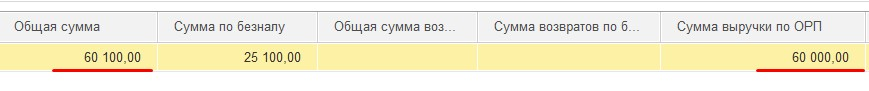
\includegraphics[width=1.0\textwidth]{12.jpg}
		\caption{<<Потерянный чек>>.}
		\label{ris:12.jpg}
	\end{figure}
	Здесь видно, что общая сумма  на 100 р. больше суммы выручки по ОРП.  (Рис.~\ref{ris:12.jpg})
	\item Первое, что  необходимо сделать - проверить по бумажным отчетом, что суммы внесены правильно. И если это действительно так и есть расхождения чисел, а не допущена ошибка ввода, приступаем к поискам потерянного чека.
	Нужно путем опроса кассиров или поиском в ОФД способом выяснить, какой товар был в этом чеке. . (Работа с сайтом ОФД изложена в п. \ref{5500})
	
	
	Установив товар в чеке или приняв решение чем его заменить нам нужно добавить этот чек в ОРП. Как  это сделать:
	
	\begin{itemize}
		\item Создать чек по нужной кассе. Записать его и с помощью ИТ отдела пересобрать ОРП.
		      Таким образом сумма выручки по ОРП сравняется с суммой по Z-отчету
	\end{itemize}
	
	
	
\end{itemize}
% Финансы

\newpage
\subsection{Формирование документа Возврат товаров поставщику}






\renewcommand{\arraystretch}{1.8} %% расстояние между строками таблицы
%\begin{landscape}
\begin{longtable}{|p{0.02\linewidth}|p{0.3\linewidth}|p{0.3\linewidth}|p{0.3\linewidth}|}
    %  {|c|c|l|c|}
    \hline
    № & \textbf{Действие} & \textbf{Ожидаемый результат} & \textbf{Фактический результат} \\
    %****************************************************************************************************
    \hline
    \hline
    \endhead
    \multicolumn{4}{|c|}{\textbf{\textit{Проверка на номенклатуру помеченную на удаление}}} \\
    \hline
    \hline
    \Rownum & Проверить, что включена константа <<крюПроверятьПомеченнуюНаУдалениеВДокументах>>  & &  \\
    \hline
    \Rownum &Перейти в раздел Закупки, выбрать <<Возвраты товаров поставщикам>>.  & 1. Открылся список документов  <<Возвраты товаров поставщикам>>;\par
    2. Отображаются все документы &  \\
    \hline
    \Rownum & Создать новый документ по кнопке \keys{Создать}  & 1. Открылась форма создания документа;\par
    2. По умолчанию в открывшейся форме заполнено поле <<Магазин>> &  \\
    \hline
    \Rownum & Заполнить реквизит <<Поставщик>> значением <<Метро>> &Заполнен <<Поставщик>> значением <<Метро>> ;    &  \\
    \hline
    \Rownum	& Нажать кнопку выбора складов & В форме выбора складов будет доступен только склад привязанный к текущему магазину  &  \\
    \hline
    \Rownum	& Выбрать склад & Заполнены реквизиты <<Склад>> и <<Организация>>  &  \\
    \hline
    \hline
    \Rownum	& Заполнить реквизит <<Причина возврата>> указав в качестве значения элемент выпадающего списка <<Возврат товара>> & Реквизит <<Причина возврата>> заполнен значением <<Возврат товара>> &  \\
    \hline
    \Rownum	& Нажать кнопку <<Добавить>> в табличной части <<Товары>>  & Откроется форма выбора справочника <<Номенклатура>>  &  \\
    \hline
    \Rownum	& Выбрать из справочника <<Номенклатура>> элемент помеченный на удаление & Заполнились поля в табличной части <<Код>>, <<Артикул>>, <<Номенклатура>>, <<Ед.изм>>, <<НДС>> &  \\
    \hline
    \Rownum	&Заполнить поле <<Количество>> значением <<1>>  & Заполнилось поле <<Количество>> &  \\
    \hline
    \Rownum	& Заполнить поле <<Цена>> значением <<1>>  & Заполнилось поле <<Цена>> &  \\
    \hline
    \Rownum	& Нажать кнопку \keys{Провести и закрыть} & 1. Программа выдает сообщение о неудачи проведения документа;\par 2. При закрытии окна сообщения в строке сообщений появляется текст ошибке с информацией, что документ содержит удаленную номенклатуру с указанием номеров строк и наименований &  \\
%****************************************************************************************************

%****************************************************************************************************

    %****************************************************************************************************

    %****************************************************************************************************
    \hline
    \hline
    \multicolumn{4}{|c|}{\textbf{\textit{Учет тары}}} \\
    \hline

    \hline
    \Rownum & Проверить, что включена константа <<крюПроводитьТару>>  & &  \\
    \hline
    \hline
    \Rownum &Перейти в раздел Закупки, выбрать <<Возвраты товаров поставщикам>>.  & 1. Открылся список документов  <<Возвраты товаров поставщикам>>;\par
    2. Отображаются все документы &  \\
    \hline
    \Rownum & Создать новый документ по кнопке \keys{Создать}  & 1. Открылась форма создания документа;\par
    2. По умолчанию в открывшейся форме заполнено поле <<Магазин>> &  \\
    \hline
    \Rownum & Заполнить реквизит <<Поставщик>> значением <<Метро>> &Заполнен <<Поставщик>> значением <<Метро>> ;    &  \\
    \hline
    \Rownum	& Нажать кнопку выбора складов & В форме выбора складов будет доступен только склад привязанный к текущему магазину  &  \\
    \hline
    \Rownum	& Выбрать склад & Заполнены реквизиты <<Склад>> и <<Организация>>  &  \\
    \hline
    \Rownum	& Заполнить реквизит <<Причина возврата>> указав в качестве значения элемент выпадающего списка <<Возврат кег>> & Реквизит <<Причина возврата>> заполнен значением <<Возврат кег>>  &  \\
    \hline
    \Rownum	& Нажать кнопку <<Добавить>> в табличной части <<Товары>>  & Откроется форма выбора справочника <<Номенклатура>>  &  \\
    \hline
    \Rownum	& Выбрать из справочника <<Номенклатура>> элемент с кодом <<00000013>> - <<КЕГ (50 л)>> & Заполнились поля в табличной части <<Код>>, <<Артикул>>, <<Номенклатура>>, <<Ед.изм>>, <<НДС>> &  \\
    \hline
    \Rownum	&Заполнить поле <<Количество>> значением <<1>>  & Заполнилось поле <<Количество>> &  \\
    \hline
    \Rownum	& Заполнить поле <<Цена>> значением <<1>>  & Заполнилось поле <<Цена>> &  \\
    \hline
    \Rownum	& Нажать кнопку \keys{Провести} &  Документ проводится без ошибок &  \\

    \hline
    \Rownum	& Выбрать команду <<Движения документа>> & Откроется отчет по движениям документа &  \\

    \hline
    \Rownum	& Найти в отчете движения по регистру <<Тара на складах>> & Движения документа по регистру накопления <<Тара на складах>> присутствуют. Измерения <<Период>>, <<Склад>>, <<Номенклатура>>, <<Поставщик>> заполнены. Значение ресурса <<Количество>> равно единице  &  \\
    \hline
    %****************************************************************************************************

    %****************************************************************************************************
    \hline
    \hline
    \multicolumn{4}{|c|}{\textbf{\textit{Очистка реквизита <<УчитыватьНДС>> и <<ЦенаВключаетНДС>>}}} \\

    \hline
    \Rownum & Проверить, что включена константа <<крюОчищатьНДСВВозвратеПоставщику>>  & &  \\

    \hline
    \Rownum &Перейти в раздел Закупки, выбрать <<Возвраты товаров поставщикам>>.  & 1. Открылся список документов  <<Возвраты товаров поставщикам>>;\par
    2. Отображаются все документы &  \\
    \hline
   \Rownum & Создать новый документ по кнопке \keys{Создать}  & 1. Открылась форма нового документа;\par
   2. По умолчанию в открывшейся форме заполнено поле <<Магазин>>\par
   3. Значение реквизитов <<ЦенаВключаетНДС>> и <<УчитыватьНДС>> на вкладке  <<Дополнительно>> равно <<Ложь>> &  \\
   \hline

    %****************************************************************************************************

     %****************************************************************************************************
    \hline
    \hline
    \multicolumn{4}{|c|}{\textbf{\textit{Печатная форма ТОРГ 12}}} \\
    \hline

    \hline
    \Rownum &Перейти в раздел Закупки, выбрать <<Возвраты товаров поставщикам>>.  & 1. Открылся список документов  <<Возвраты товаров поставщикам>>;\par
    2. Отображаются все документы &  \\
    \hline
    \Rownum & Открыть любой существующий документ  & 1. Открылась форма существующего документа;\par
     &  \\
     \hline
    \Rownum	& По кнопке выбора печатных форм выбрать <<ТОРГ-12(Товарная накладная на возврат)>>  & Сформировалась печатная форма &  \\
    \hline
    \Rownum	& Проверить представление организации и поле <<Вид операции>> в шапке & 1. В представлении организации присутствует КПП организации\par
    2. Поле <<Вид операции>> заполнено значением <<Возврат>>  &  \\


    %****************************************************************************************************





    \hline
    \Rownum	& test &  &  \\ %\nopagebreak Для запрещения разбиения страниц применяется команда \nopagebreak сразу после двух слешей в конце строчки.
    \hline
\end{longtable}
\newpage
\section{Возможные проблемы}

\begin{itemize}	
	\item  \stСитуация, когда на кассах будет разное время, достаточно нескольких секунд. И тогда какая-то из открытых смен может не попасть в УНФ, если по времени кассы она открылась раньше уже зафиксированной даты, а по текущему времени позже.

\end{itemize}
% ЕГАИС


\newpage
\section{Продажи}
\subsection{Объекты тестирования, описанные в разделе}

\begin{tabular}{p{0.05\linewidth}p{0.4\linewidth}p{0.4\linewidth}}
    \toprule
    %	\hline
    1 & Вид объекта & Документ \\
    \hline
    & Имя & ОтчетОРозничныхПродажах \\
    \hline
    & Синоним  & Отчет о розничных продажах \\
    \hline
    2 & Вид объекта  & Документ \\
    \hline
    & Имя & КассоваяСмена \\
    \hline
    & Синоним  & Кассовая смена \\
    \hline
    3 & Вид объекта  & Документ \\
    \hline
    & Имя & ВозвратТоваровОтПокупателя \\
    \hline
    & Синоним  & Возврат товаров от покупателя \\
    \hline

    \bottomrule %%% верхняя линейка
\end{tabular}
\newpage
\subsection{Формирование документа Отчет о розничных продажах}

\renewcommand{\arraystretch}{1.8} %% расстояние между строками таблицы
%\begin{landscape}
%****************************************************************************************************
\begin{longtable}{|p{0.02\linewidth}|p{0.3\linewidth}|p{0.3\linewidth}|p{0.3\linewidth}|}
    %  {|c|c|l|c|}
    \hline
    № & \textbf{Действие} & \textbf{Ожидаемый результат} & \textbf{Фактический результат} \\
    \hline
    \hline
    \endhead
    \multicolumn{4}{|c|}{\textbf{\textit{Проверка блокировки проведения документа в центральном узле}}} \\
    \hline
    \hline
    \Rownum & Запустить конфигурацию главного узла РИБ  & Запущен ЦУ узел &  \\
    \hline
    \Rownum &Перейти в раздел <<Продажи>>, выбрать <<Отчеты о розничных продажах>>.  & 1. Открылся список документов  <<Отчеты о розничных продажах>>;\par
    2. Отображаются все документы &  \\
    \hline
    \Rownum & Открыть любой проведенный документ & Открылась форма проведенного документа;\par
    &  \\
    \hline
    \Rownum & Нажать кнопку \keys{Провести и закрыть} & 1. Выходит сообщение об ошибке <<Документ Отчет о розничных продажах можно проводить только в том узле, в котором он создан>> ;\par
    2. Документ не проводится  &  \\
    \hline

    %****************************************************************************************************


\end{longtable}
%****************************************************************************************************


%****************************************************************************************************
\begin{longtable}{|p{0.02\linewidth}|p{0.3\linewidth}|p{0.3\linewidth}|p{0.3\linewidth}|}
    %  {|c|c|l|c|}
    \hline
    № & \textbf{Действие} & \textbf{Ожидаемый результат} & \textbf{Фактический результат} \\
    \hline
    \hline
    \endhead
    \multicolumn{4}{|c|}{\textbf{\textit{Проверка проведения документа в узле магазина}}} \\
    \hline
    \hline
    \Rownum & Запустить конфигурацию  узла магазина  & Запущен узел магазина &  \\
    \hline
    \Rownum &Перейти в раздел <<Продажи>>, выбрать <<Отчеты о розничных продажах>>.  & 1. Открылся список документов  <<Отчеты о розничных продажах>>;\par
    2. Отображаются все документы &  \\
    \hline
    \Rownum & Открыть любой проведенный документ & Открылась форма проведенного документа;\par
    &  \\
    \hline
    \Rownum & Нажать кнопку \keys{Провести и закрыть} &  Документ  проводится  &  \\
    \hline

\end{longtable}
%****************************************************************************************************


%****************************************************************************************************
\begin{longtable}{|p{0.02\linewidth}|p{0.3\linewidth}|p{0.3\linewidth}|p{0.3\linewidth}|}
    %  {|c|c|l|c|}
    \hline
    № & \textbf{Действие} & \textbf{Ожидаемый результат} & \textbf{Фактический результат} \\
    \hline
    \hline
    \endhead
    \multicolumn{4}{|c|}{\textbf{\textit{Проверка создания документа <<Сборка товаров>>}}} \\
    \hline
    \hline
    \Rownum & Запустить конфигурацию главного узла РИБ  & Запущен ЦУ узел &  \\
    \hline
    \Rownum &Перейти в раздел <<Продажи>>, выбрать <<Отчеты о розничных продажах>>.  & 1. Открылся список документов  <<Отчеты о розничных продажах>>;\par
    2. Отображаются все документы &  \\
    \hline
    \Rownum & Создать новый документ по кнопке \keys{Создать}  & 1. Открылась форма создания документа;\par
    2. По умолчанию в открывшейся форме заполнено только поле <<Дата>> &  \\
    \hline
    \Rownum & Заполнить реквизит <<Касса (ККМ)>> значением с кодом <<ШТ-000004>>, <<75\_№2 (Кулинария) Шмидта 9>> &Заполнен реквизит <<Касса (ККМ)>> и <<Магазин>> ;    &  \\
    \hline
    \Rownum	& Нажать кнопку <<Добавить>> в табличной части <<Товары>>  & Откроется форма выбора справочника <<Номенклатура>>  &  \\
    \hline

    \Rownum	& Выбрать из справочника <<Номенклатура>> элемент с кодом <<КН000793>> - <<Гренки чесночные>> & Заполнились поля в табличной части <<Код>>, <<Артикул>>, <<Номенклатура>>, <<Ед.изм>>,<<Цена>>,<<Склад>>, <<НДС>> &  \\
    \hline
    \Rownum	&Заполнить поле <<Количество>> значением <<0,200>>  & Заполнилось поле <<Количество>> &  \\
    \hline
    \Rownum	& Нажать кнопку \keys{Провести} &  Документ проводится без ошибок &  \\
    \hline
    \Rownum	& Выбрать команду <<Связанные документы>> & Откроется отчет <<Связанные документы>> &  \\
    \hline
    \Rownum	& Найти в отчете документ <<Сборка товаров>>, открыть его & 1. Документ <<Сборка товаров>> открыт;\par
    2. Все реквизиты заполнены ;\par
    3. Значение реквизита <<Номенклатура>>  равно <<Гренки чесночные>>;\par
    4. Значение реквизита <<Количество>> равно <<0,200>>;\par
    5. Документ проведен. &  \\
    \hline

\end{longtable}
%****************************************************************************************************


%\begin{verbatim}
%Если  (Константы.крюКонролироватьПроведениеОРП.Получить()) И  (ПланыОбмена.ГлавныйУзел() = Неопределено) Тогда
%    Сообщить("Документ Отчет о розничных продажах можно проводить только в том узле, в котором он создан");
%    Отказ = Истина;
%КонецЕсли;
%
%\end{verbatim}

%\begin{algorithmic}[1]
%    \IF{\(i\leqslant0\)} \STATE \(i\gets1\) \ELSE
%    \IF{\(i\geqslant0\)} \STATE \(i\gets0\)
%    \COMMENT{смысла в этом алгоритме не ищите}
%    \ENDIF
%    \ENDIF
%    \ENSURE \(i\geqslant0\)
%    \FORALL{\(\xi \in \mathcal{A}\)}
%    \STATE \(\mathcal{B}\gets\xi^2\)
%    \ENDFOR
%    \RETURN \(\mathcal{B}\)
%\end{algorithmic} % Справочники
\newpage
\subsection{Формирование документа Кассовая смена}

\renewcommand{\arraystretch}{1.8} %% расстояние между строками таблицы
%\begin{landscape}
\begin{longtable}{|p{0.02\linewidth}|p{0.3\linewidth}|p{0.3\linewidth}|p{0.3\linewidth}|}
    %  {|c|c|l|c|}
    \hline
    № & \textbf{Действие} & \textbf{Ожидаемый результат} & \textbf{Фактический результат} \\
    %****************************************************************************************************
    \hline
    \hline
    \endhead
    \multicolumn{4}{|c|}{\textbf{\textit{******}}} \\
    \hline
    \hline

    %****************************************************************************************************


\end{longtable}
\newpage
\subsection{Формирование документа Возврат товаров от покупателя}

\renewcommand{\arraystretch}{1.8} %% расстояние между строками таблицы
%\begin{landscape}
%****************************************************************************************************
\begin{longtable}{|p{0.02\linewidth}|p{0.3\linewidth}|p{0.3\linewidth}|p{0.3\linewidth}|}
    %  {|c|c|l|c|}
    \hline
    № & \textbf{Действие} & \textbf{Ожидаемый результат} & \textbf{Фактический результат} \\
    \hline
    \hline
    \endhead
    \multicolumn{4}{|c|}{\textbf{\textit{Проверка корректного заполнения глобальное переменной <<НомерДокументаКассыККМ>>}}} \\
    \hline
    \hline
    \Rownum & Запустить конфигурацию главного узла РИБ  & Запущен ЦУ узел &  \\
    \hline
 \end{longtable}
%****************************************************************************************************


%****************************************************************************************************
\begin{longtable}{|p{0.02\linewidth}|p{0.3\linewidth}|p{0.3\linewidth}|p{0.3\linewidth}|}
    %  {|c|c|l|c|}
    \hline
    № & \textbf{Действие} & \textbf{Ожидаемый результат} & \textbf{Фактический результат} \\
    \hline
    \hline
    \endhead
    \multicolumn{4}{|c|}{\textbf{\textit{Проверка процедуры печати чека с учетом двух касс}}} \\
    \hline
    \hline
    \Rownum & Запустить конфигурацию главного узла РИБ  & Запущен ЦУ узел &  \\
    \hline
\end{longtable}
%****************************************************************************************************
% Возврат товаров от покупателя
\newpage

\section{Склад}
\subsection{Объекты тестирования, описанные в разделе}

\begin{longtable}{p{0.05\linewidth}p{0.4\linewidth}p{0.4\linewidth}}
  %  \toprule
    	\hline
    1 & Вид объекта & Документ \\
    \hline
%     \hline
%    \endhead
    & Имя & ОприходованиеТоваров \\
     \hline
       & Синоним  & Оприходование товаров \\
    \hline
    2 & Вид объекта  & Документ \\
    \hline
    & Имя & СписаниеТоваров \\
    \hline
    & Синоним  & Списание товаров \\
    \hline
    3 & Вид объекта  & Документ \\
    \hline
    & Имя & ПересчетТоваров \\
    \hline
    & Синоним  & Пересчет товаров \\
    \hline
    4 & Вид объекта  & Документ \\
   \hline
   & Имя & СборкаТоваров \\
   \hline
   & Синоним  & Сборка товаров \\
   \hline
   5 & Вид объекта  & Документ \\
   \hline
   & Имя & ПриходныйОрдерНаТовары \\
   \hline
   & Синоним  & Приходный ордер на товары \\
   \hline
    6 & Вид объекта  & Документ \\
   \hline
   & Имя & РасходныйОрдерНаТовары \\
   \hline
   & Синоним  & Расходный ордер на товары \\
   \hline
   7 & Вид объекта  & Документ \\
   \hline
   & Имя & АктПостановкиНаБалансЕГАИС \\
   \hline
   & Синоним  & Акт постановки на баланс ЕГАИС \\
   \hline
    8 & Вид объекта  & Документ \\
   \hline
   & Имя & АктСписанияЕГАИС \\
   \hline
   & Синоним  & Акт списания ЕГАИС \\
   \hline
    9 & Вид объекта  & Документ \\
   \hline
   & Имя & ПередачаВРегистр2ЕГАИС \\
   \hline
   & Синоним  & Передача в регистр №2 ЕГАИС \\
   \hline
    10 & Вид объекта  & Документ \\
   \hline
   & Имя & ВозвратИзРегистра2ЕГАИС \\
   \hline
   & Синоним  & Возврат из регистра №2 ЕГАИС \\
   \hline
    \bottomrule %%% верхняя линейка
\end{longtable}% Склад
\newpage
\subsection{Формирование документа Оприходование товаров}

\renewcommand{\arraystretch}{1.8} %% расстояние между строками таблицы
%\begin{landscape}
%****************************************************************************************************
\begin{longtable}{|p{0.02\linewidth}|p{0.3\linewidth}|p{0.3\linewidth}|p{0.3\linewidth}|}
    %  {|c|c|l|c|}
    \hline
    № & \textbf{Действие} & \textbf{Ожидаемый результат} & \textbf{Фактический результат} \\
    \hline
    \hline
    \endhead
    \multicolumn{4}{|c|}{\textbf{\textit{Проверка процедуры печати чека с учетом двух касс}}} \\
    \hline
    \hline
    \Rownum & Запустить конфигурацию главного узла РИБ  & Запущен ЦУ узел &  \\
    \hline
\end{longtable}
%****************************************************************************************************
 % Оприходование товаров
\newpage
\subsection{Формирование документа Списание товаров}

    \renewcommand{\arraystretch}{1.8} %% расстояние между строками таблицы
%\begin{landscape}
\begin{longtable}{|p{0.02\linewidth}|p{0.3\linewidth}|p{0.3\linewidth}|p{0.3\linewidth}|}
    %  {|c|c|l|c|}
    \hline
    № & \textbf{Действие} & \textbf{Ожидаемый результат} & \textbf{Фактический результат} \\
    %****************************************************************************************************
    \hline
    \hline
    \endhead
    \multicolumn{4}{|c|}{\textbf{\textit{Проверка на номенклатуру помеченную на удаление}}} \\
    \hline
    \hline
    \Rownum & Проверить, что включена константа <<крюПроверятьПомеченнуюНаУдалениеВДокументах>>  & &  \\
    \hline
    \Rownum &Перейти в раздел Склад, выбрать <<Списание товаров>>.  & 1. Открылся список документов  <<Списание товаров>>;\par
    2. Отображаются все документы &  \\
    \hline
    \Rownum & Создать новый документ по кнопке \keys{Создать}  & 1. Открылась форма создания документа;\par
    2. По умолчанию в открывшейся форме заполнено поле <<Магазин>> &  \\
    \hline
    \Rownum & Заполнить реквизит <<Склад>> значением соответствующим выбранному магазину &Заполнен <<Склад отправитель>> и <<Организация>> ;    &  \\
    \hline
    \Rownum	& Заполнить реквизит <<Аналитика хоз. операции>> значением <<Оприходование товаров (ВОЗВРАТ ОТ ПОКУПАТЕЛЯ)>> & Заполны реквизиты: 1. <<Магазин>> значением <<75. Шмидта 9, Новосибирск>>;\par
    2. <<Склад>> значением <<75. Шмидта 9, Новосибирск>>;\par
    3. <<Организация>> значением <<ООО "КРЮГЕР ХАУС" КОЛЬЦОВО (Новосибирск, Шмидта ул, 9)>>;\par
    4. <<Аналитика хоз. операции>> значением <<Списание на затраты (ВОЗВРАТ ОТ ПОКУПАТЕЛЯ-ЗАМЕНА)>>  &  \\
    \hline
    \Rownum	& Нажать кнопку <<Добавить>> в табличной части <<Товары>>  & Откроется форма выбора справочника <<Номенклатура>>  &  \\
    \hline
    \Rownum	& Выбрать из справочника <<Номенклатура>> элемент помеченный на удаление & Заполнились поля в табличной части <<Код>>, <<Артикул>>, <<Номенклатура>>, <<Ед.изм>> &  \\
    \hline
    \Rownum	&Заполнить поле <<Количество>> значением <<1>>  & Заполнилось поле <<Количество>> &  \\
    \hline
    \Rownum	& Заполнить поле <<Цена>> значением <<1>>  & 1. Заполнилось поле <<Цена>>;\par
    2. Заполнилось поле <<Сумма>> &  \\
    \hline
    \Rownum	& Нажать кнопку \keys{Провести и закрыть} & 1. Программа выдает сообщение о неудаче проведения документа;\par 2. При закрытии окна сообщения в строке сообщений появляется текст ошибке с информацией, что документ содержит удаленную номенклатуру с указанием номеров строк и наименований &  \\
    \hline
    %****************************************************************************************************



    %****************************************************************************************************

    \multicolumn{4}{|c|}{\textbf{\textit{Учет тары}}} \\
    %   \hline
    \hline
    \Rownum & Проверить, что включена константа <<крюПроводитьТару>>  & &  \\
    \hline
    \Rownum &Перейти в раздел Склад, выбрать <<Списание товаров>>.  & 1. Открылся список документов  <<Списание товаров>>;\par
    2. Отображаются все документы &  \\
    \hline
    \Rownum & Создать новый документ по кнопке \keys{Создать}  & 1. Открылась форма нового документа;\par
    2. По умолчанию в открывшейся форме заполнено поле <<Магазин>> &  \\
    \hline
    \Rownum & Заполнить реквизит <<Склад>> значением соответствующим выбранному магазину &Заполнен <<Склад отправитель>> и <<Организация>> ;    &  \\
    \hline
    \Rownum	& Заполнить реквизит <<Аналитика хоз. операции>> значением <<Оприходование товаров (ВОЗВРАТ ОТ ПОКУПАТЕЛЯ)>> & Заполны реквизиты: 1. <<Магазин>> значением <<75. Шмидта 9, Новосибирск>>;\par
    2. <<Склад>> значением <<75. Шмидта 9, Новосибирск>>;\par
    3. <<Организация>> значением <<ООО "КРЮГЕР ХАУС" КОЛЬЦОВО (Новосибирск, Шмидта ул, 9)>>;\par
    4. <<Аналитика хоз. операции>> значением <<Списание на затраты (ВОЗВРАТ ОТ ПОКУПАТЕЛЯ-ЗАМЕНА)>>  &  \\
    \hline
    \Rownum	& Нажать кнопку <<Добавить>> в табличной части <<Товары>>  & Откроется форма выбора справочника <<Номенклатура>>  &  \\
    \hline
    \Rownum	& Выбрать из справочника <<Номенклатура>> элемент с кодом <<00000013>> - <<КЕГ (50 л)>> & Заполнились поля в табличной части <<Код>>, <<Артикул>>, <<Номенклатура>>, <<Ед.изм>> &  \\
    \hline
    \Rownum	&Заполнить поле <<Количество>> значением <<1>>  & Заполнилось поле <<Количество>> &  \\
    \hline
    \Rownum	& Заполнить поле <<Цена>> значением <<1>>  & Заполнилось поле <<Цена>>;\par
    2. Заполнилось поле <<Сумма>> &  \\
    \hline
    \Rownum	& Нажать кнопку \keys{Провести и закрыть} & 1. Программа выдает сообщение о неудаче проведения документа;\par 2. При закрытии окна сообщения в строке сообщений появляется текст ошибке с информацией, что документ содержит возвратную тару или оборудование с указанием номеров строк &  \\
    \hline
    %****************************************************************************************************
\end{longtable}



% Списание товаров
\newpage
\subsection{Формирование документа Пересчет товаров}

\renewcommand{\arraystretch}{1.8} %% расстояние между строками таблицы
%\begin{landscape}
\begin{longtable}{|p{0.02\linewidth}|p{0.3\linewidth}|p{0.3\linewidth}|p{0.3\linewidth}|}
    %  {|c|c|l|c|}
    \hline
    № & \textbf{Действие} & \textbf{Ожидаемый результат} & \textbf{Фактический результат} \\
    %****************************************************************************************************
    \hline
    \hline
    \endhead
    \multicolumn{4}{|c|}{\textbf{\textit{******}}} \\
    \hline
    \hline

    %****************************************************************************************************


\end{longtable}% Пересчет товаров
\newpage
\subsection{Формирование документа Сборка товаров}

\renewcommand{\arraystretch}{1.8} %% расстояние между строками таблицы
%\begin{landscape}
\begin{longtable}{|p{0.02\linewidth}|p{0.3\linewidth}|p{0.3\linewidth}|p{0.3\linewidth}|}
    %  {|c|c|l|c|}
    \hline
    № & \textbf{Действие} & \textbf{Ожидаемый результат} & \textbf{Фактический результат} \\
    %****************************************************************************************************
    \hline
    \hline
    \endhead
    \multicolumn{4}{|c|}{\textbf{\textit{******}}} \\
    \hline
    \hline

    %****************************************************************************************************


\end{longtable}% Сборка товаров
\newpage
\subsection{Формирование документа Приходный ордер на товары}

\renewcommand{\arraystretch}{1.8} %% расстояние между строками таблицы
    %\begin{landscape}
\begin{longtable}{|p{0.02\linewidth}|p{0.3\linewidth}|p{0.3\linewidth}|p{0.3\linewidth}|}
    %  {|c|c|l|c|}
    \hline
    № & \textbf{Действие} & \textbf{Ожидаемый результат} & \textbf{Фактический результат} \\
    %****************************************************************************************************
    \hline
    \hline
    \endhead
    \multicolumn{4}{|c|}{\textbf{\textit{Проверка на номенклатуру помеченную на удаление}}} \\
    \hline
    \hline
    \Rownum & Проверить, что включена константа <<крюПроверятьПомеченнуюНаУдалениеВДокументах>>  & &  \\
    \hline
    \Rownum &Перейти в раздел Склад, выбрать <<Приемка>>.  & 1. Открылся список документов  <<Приходные ордера на товары>>;\par
    2. Отображаются все документы &  \\
    \hline
    \Rownum & Открыть существующий документ  & 1. Открылась форма существующего документа
    &  \\

    \hline
    \Rownum	& Нажать кнопку <<Добавить>> в табличной части <<Товары>>  & Откроется форма выбора справочника <<Номенклатура>>  &  \\
    \hline
    \Rownum	& Выбрать из справочника <<Номенклатура>> элемент помеченный на удаление & Заполнились поля в табличной части <<Код>>, <<Артикул>>, <<Номенклатура>>, <<Ед.изм>> &  \\
    \hline
    \Rownum	&Заполнить поле <<Количество>> значением <<1>>  & Заполнилось поле <<Количество>> &  \\
    \hline
    \Rownum	& Нажать кнопку \keys{Провести и закрыть} & 1. Программа выдает сообщение о неудаче проведения документа;\par 2. При закрытии окна сообщения в строке сообщений появляется текст ошибке с информацией, что документ содержит удаленную номенклатуру с указанием номеров строк и наименований &  \\
    \hline
    %****************************************************************************************************



    %****************************************************************************************************

    \multicolumn{4}{|c|}{\textbf{\textit{Учет тары}}} \\
    %   \hline
    \hline
    \Rownum & Проверить, что включена константа <<крюПроводитьТару>>  & &  \\
    \hline
    \Rownum &Перейти в раздел Склад, выбрать <<Приемка>>.  & 1. Открылся список документов  <<Приходные ордера на товары>>;\par
    2. Отображаются все документы &  \\
    \hline
    \Rownum & Открыть существующий документ  & 1. Открылась форма существующего документа
    &  \\
    \hline
    \Rownum	& Нажать кнопку <<Добавить>> в табличной части <<Товары>>  & Откроется форма выбора справочника <<Номенклатура>>  &  \\
    \hline
    \Rownum	& Выбрать из справочника <<Номенклатура>> элемент с кодом <<00000013>> - <<КЕГ (50 л)>> & Заполнились поля в табличной части <<Код>>, <<Артикул>>, <<Номенклатура>>, <<Ед.изм>> &  \\
    \hline
    \Rownum	&Заполнить поле <<Количество>> значением <<1>>  & Заполнилось поле <<Количество>> &  \\

    \Rownum	& Нажать кнопку \keys{Провести и закрыть} & 1. Программа выдает сообщение о неудаче проведения документа;\par 2. При закрытии окна сообщения в строке сообщений появляется текст ошибке с информацией, что документ содержит возвратную тару или оборудование с указанием номеров строк &  \\
    \hline
    %****************************************************************************************************
\end{longtable}



 % Приходный ордер на товары
\newpage
\subsection{Формирование документа Расходный ордер на товары}

\renewcommand{\arraystretch}{1.8} %% расстояние между строками таблицы
%\begin{landscape}
\begin{longtable}{|p{0.02\linewidth}|p{0.3\linewidth}|p{0.3\linewidth}|p{0.3\linewidth}|}
    %  {|c|c|l|c|}
    \hline
    № & \textbf{Действие} & \textbf{Ожидаемый результат} & \textbf{Фактический результат} \\
    %****************************************************************************************************
    \hline
    \hline
    \endhead
    \multicolumn{4}{|c|}{\textbf{\textit{Проверка на номенклатуру помеченную на удаление}}} \\
    \hline
    \hline
    \Rownum & Проверить, что включена константа <<крюПроверятьПомеченнуюНаУдалениеВДокументах>>  & Значение константы - Истина &  \\
    \hline
    \Rownum &Перейти в раздел Склад, выбрать <<Отгрузка>>.  & 1. Открылся список документов  <<Расходные ордера на товары>>;\par
    2. Отображаются все документы &  \\
    \hline
    \Rownum & Открыть существующий документ  & 1. Открылась форма существующего документа
    &  \\

    \hline
    \Rownum	& Нажать кнопку <<Добавить>> в табличной части <<Товары>>  & Откроется форма выбора справочника <<Номенклатура>>  &  \\
    \hline
    \Rownum	& Выбрать из справочника <<Номенклатура>> элемент помеченный на удаление & Заполнились поля в табличной части <<Код>>, <<Артикул>>, <<Номенклатура>>, <<Ед.изм>> &  \\
    \hline
    \Rownum	&Заполнить поле <<Количество>> значением <<1>>  & Заполнилось поле <<Количество>> &  \\
    \hline
    \Rownum	& Нажать кнопку \keys{Провести и закрыть} & 1. Программа выдает сообщение о неудаче проведения документа;\par 2. При закрытии окна сообщения в строке сообщений появился текст ошибке с информацией, что документ содержит удаленную номенклатуру с указанием номеров строк и наименований &  \\
    \hline
    %****************************************************************************************************



    %****************************************************************************************************

    \multicolumn{4}{|c|}{\textbf{\textit{Учет тары}}} \\
    %   \hline
    \hline
    \Rownum & Проверить, что включена константа <<крюПроводитьТару>>  & Значение константы - Истина &  \\
    \hline
    \Rownum &Перейти в раздел Склад, выбрать <<Отгрузка>>.  & 1. Открылся список документов  <<Расходные ордера на товары>>;\par
    2. Отображаются все документы &  \\
    \hline
    \Rownum & Открыть существующий документ  & 1. Открылась форма существующего документа
    &  \\
    \hline
    \Rownum	& Нажать кнопку <<Добавить>> в табличной части <<Товары>>  & Откроется форма выбора справочника <<Номенклатура>>  &  \\
    \hline
    \Rownum	& Выбрать из справочника <<Номенклатура>> элемент с кодом <<00000013>> - <<КЕГ (50 л)>> & Заполнились поля в табличной части <<Код>>, <<Артикул>>, <<Номенклатура>>, <<Ед.изм>> &  \\
    \hline
    \Rownum	&Заполнить поле <<Количество>> значением <<1>>  & Заполнилось поле <<Количество>> &  \\

    \Rownum	& Нажать кнопку \keys{Провести и закрыть} & 1. Программа выдает сообщение о неудаче проведения документа;\par 2. При закрытии окна сообщения в строке сообщений появился текст ошибке с информацией, что документ содержит возвратную тару или оборудование с указанием номеров строк &  \\
    \hline
    %****************************************************************************************************
\end{longtable}
% Расходный ордер на товары
\newpage



\section{Финансы}
\subsection{Объекты тестирования, описанные в разделе}

\begin{longtable}{p{0.05\linewidth}p{0.4\linewidth}p{0.4\linewidth}}
    %  \toprule
    \hline
    1 & Вид объекта & Документ \\
    \hline
    %     \hline
    %    \endhead
    & Имя & ПриходныйКассовыйОрдер \\
    \hline
    & Синоним  & Приходный кассовый ордер \\
    \hline
    2 & Вид объекта  & Документ \\
    \hline
    & Имя & РасходныйКассовыйОрдер \\
    \hline
    & Синоним  & Расходный кассовый ордер \\
    \hline
    3 & Вид объекта  & Документ \\
    \hline
    & Имя & ЗарплатаКВыплатеОрганизаций \\
    \hline
    & Синоним  & Зарплата к выплате организаций \\
    \hline

    \bottomrule %%% верхняя линейка
\end{longtable}
\newpage
\subsection{Формирование документа Приходный кассовый ордер}

\renewcommand{\arraystretch}{1.8} %% расстояние между строками таблицы
%\begin{landscape}
\begin{longtable}{|p{0.02\linewidth}|p{0.3\linewidth}|p{0.3\linewidth}|p{0.3\linewidth}|}
    %  {|c|c|l|c|}
    \hline
    № & \textbf{Действие} & \textbf{Ожидаемый результат} & \textbf{Фактический результат} \\
    %****************************************************************************************************
    \hline
    \hline
    \endhead
    \multicolumn{4}{|c|}{\textbf{\textit{Создание на основании РКО}}} \\
    \hline
    \Rownum &Перейти в раздел <<Финансы>>, выбрать <<Расходные кассовые ордера>>.  & 1. Открылся список документов  <<Расходные кассовые ордера>>;\par
    2. Отображаются все документы &  \\
    \hline
    \Rownum & Открыть существующий документ с операцией <<Прочие расходы>>  & 1. Открылась форма существующего документа
    &  \\

    \hline
    \Rownum	& Нажать кнопку <<Создать на основании>>  & Появился выпадающий список с вариантами документов   &  \\
    \hline
    \Rownum	& Выбрать <<Приходный кассовый ордер>> & 1. Открылась форма нового документа <<Приходный кассовый ордер>>;\par
    2. Заполнены реквизиты <<Дата документа>>, <<Контрагент>>, <<Сумма документа>>, <<Операция>>;\par
    3. Создание нового документа <<Приходный кассовый ордер>> на основании текущего <<Расходного кассового ордера>> успешно &  \\
    \hline
    %****************************************************************************************************



    %****************************************************************************************************

    \multicolumn{4}{|c|}{\textbf{\textit{Сё}}} \\
     \hline

    \Rownum &Перейти в раздел Склад, выбрать <<Отгрузка>>.  & 1. Открылся список документов  <<Расходные ордера на товары>>;\par
    2. Отображаются все документы &  \\
    \hline
    \Rownum & Открыть существующий документ  & 1. Открылась форма существующего документа
    &  \\
    \hline
    \Rownum	& Нажать кнопку <<Добавить>> в табличной части <<Товары>>  & Откроется форма выбора справочника <<Номенклатура>>  &  \\
    \hline
    \Rownum	& Выбрать из справочника <<Номенклатура>> элемент с кодом <<00000013>> - <<КЕГ (50 л)>> & Заполнились поля в табличной части <<Код>>, <<Артикул>>, <<Номенклатура>>, <<Ед.изм>> &  \\
    \hline
    \Rownum	&Заполнить поле <<Количество>> значением <<1>>  & Заполнилось поле <<Количество>> &  \\

    \Rownum	& Нажать кнопку \keys{Провести и закрыть} & 1. Программа выдает сообщение о неудаче проведения документа;\par 2. При закрытии окна сообщения в строке сообщений появляется текст ошибке с информацией, что документ содержит возвратную тару или оборудование с указанием номеров строк &  \\
    \hline
    %****************************************************************************************************
\end{longtable}
 % Приходно кассовый ордер
\newpage
\subsection{Формирование документа Расходный кассовый ордер}

\renewcommand{\arraystretch}{1.8} %% расстояние между строками таблицы
\begin{longtable}{|p{0.02\linewidth}|p{0.3\linewidth}|p{0.3\linewidth}|p{0.3\linewidth}|}
    %  {|c|c|l|c|}
    \hline
    № & \textbf{Действие} & \textbf{Ожидаемый результат} & \textbf{Фактический результат} \\
    %****************************************************************************************************
    \hline
    \hline
    \endhead
      \multicolumn{4}{|c|}{\textbf{\textit{Проверка появления реквизита <<крюБанкВноситель>>}}} \\
   \hline
   \Rownum &Перейти в раздел <<Финансы>>, выбрать <<Расходные кассовые ордера>>.  & 1. Открылся список документов  <<Расходные кассовые ордера>>;\par
   2. Отображаются все документы &  \\
   \hline
   \Rownum & Создать новый документ с видом операции <<Сдача ДС в банк>> по кнопке \keys{Создать}  & 1. Открылась форма создания документа;\par
   2. По умолчанию в открывшейся форме заполнено поле <<Операция>>, <<Дата документа>>;\par
   3. В шапке документа присутствует реквизит <<Банк-вноситель>> &  \\
   \hline
    %****************************************************************************************************



    %****************************************************************************************************

       \hline
   \hline

%   \multicolumn{4}{|c|}{\textbf{\textit{Добавляется печатная форма «ПечатьПрепроводительнаяВедомостьНакладнаяКСумке»}}} \\
%   \hline
%
%
%   %****************************************************************************************************
%
%
%   \multicolumn{4}{|c|}{\textbf{\textit{Изменено заполнение параметра печати «НаименованиеБанкаВносителя\_БИК» для инкассации.}}} \\
%
%
%   %****************************************************************************************************
%
%   \hline
%
%   \multicolumn{4}{|c|}{\textbf{\textit{Добавлено заполнение структуры для заполнение печатных форм РКО}}} \\
%
%
%   %****************************************************************************************************
%
%   \hline
%
%   \multicolumn{4}{|c|}{\textbf{\textit{При изменении кассы корректно заполняется значение глобальной переменной НомерДокументаКассыККМ}}} \\
%
%
%   %****************************************************************************************************
%
%   \hline
%
%   \multicolumn{4}{|c|}{\textbf{\textit{Корректно устанавливается номер чека ККМ при печати чека "Клиент"с учетом наших двух касс}}} \\
%
%
%   %****************************************************************************************************
%     %****************************************************************************************************
%
%   \hline
%
%   \multicolumn{4}{|c|}{\textbf{\textit{Корректно устанавливается номер чека ККМ при печати чека «КлиентИнкассация» с учетом наших двух касс}}} \\
%
%    %****************************************************************************************************
%
%    \hline
%
%    \multicolumn{4}{|c|}{\textbf{\textit{При открытии документа корректно заполняется значение глобальной переменной НомерДокументаКассыККМ с учетом нашего разделения на две кассы.}}} \\
%    \hline
%
%    %****************************************************************************************************
\end{longtable}

\newpage
\subsection{Формирование документа Зарплата к выплате организаций}

\renewcommand{\arraystretch}{1.8} %% расстояние между строками таблицы
%\begin{landscape}
\begin{longtable}{|p{0.02\linewidth}|p{0.3\linewidth}|p{0.3\linewidth}|p{0.3\linewidth}|}
    %  {|c|c|l|c|}
    \hline
    № & \textbf{Действие} & \textbf{Ожидаемый результат} & \textbf{Фактический результат} \\
    %****************************************************************************************************
    \hline
    \hline
    \endhead
    \multicolumn{4}{|c|}{\textbf{\textit{В табличную часть "Зарплата"добавлен реквизит «КлючСтроки» для использования при обмене с УТ}}} \\
    \hline
    \hline

    %****************************************************************************************************


\end{longtable}% Зарплата к выплате организаций
\newpage
\section{Маркетинг}
\subsection{Объекты тестирования, описанные в разделе}

\begin{longtable}{p{0.05\linewidth}p{0.4\linewidth}p{0.4\linewidth}}
    %  \toprule
    \hline
    1 & Вид объекта & Документ \\
    \hline
    %     \hline
    %    \endhead
    & Имя & УстановкаЦенНоменклатуры \\
    \hline
    & Синоним  & Установка цен номенклатуры \\
    \hline
    2 & Вид объекта  & Подсистема \\
    \hline
    & Имя & Дисконт \\
    \hline
    & Синоним  & Дисконт \\
    \hline

    \bottomrule %%% верхняя линейка
\end{longtable}
\newpage
\subsection{Формирование документа Установка цен номенклатуры}

\renewcommand{\arraystretch}{1.8} %% расстояние между строками таблицы
%\begin{landscape}
\begin{longtable}{|p{0.02\linewidth}|p{0.3\linewidth}|p{0.3\linewidth}|p{0.3\linewidth}|}
    %  {|c|c|l|c|}
    \hline
    № & \textbf{Действие} & \textbf{Ожидаемый результат} & \textbf{Фактический результат} \\
    %****************************************************************************************************
    \hline
    \hline
    \endhead
    \multicolumn{4}{|c|}{\textbf{\textit{Механизм заполнения цен}}} \\
    \hline
       \hline
   \Rownum &  Перейти в раздел Склад, выбрать <<Возвраты из регистра №2>>.  & 1. Открылся список документов  <<Возвраты из регистра №2>>;\par
   2. Отображаются все документы &  \\
   \hline
   \Rownum & Открыть существующий документ  & 1. Открылась форма существующего документа
   &  \\
   \hline
   \Rownum	& Нажать кнопку \keys{Провести} &  Документ проводится без ошибок &  \\
   \hline
   \Rownum	& Выбрать команду <<Движения документа>> & Откроется отчет по движениям документа &  \\
   \hline
   \Rownum	& Найти в отчете движения по регистру <<Остатки алкогольной продукции в торговом зале ЕГАИС>> & Движения документа по регистру сведений <<Остатки алкогольной продукции в торговом зале ЕГАИС>> присутствуют. Измерения <<Период>>, <<Организация ЕГАИС>>,<<Склад>>, <<Номенклатура>>, <<Алкогольная продукция>>, <<Справка Б>>, <<Документ приход>> заполнены. Значение ресурса <<Количество упаковок>> заполнено  &  \\
   \hline

    %****************************************************************************************************


\end{longtable} % Установка цен номенклатуры
\newpage
\subsection{Механизм дисконта}

\renewcommand{\arraystretch}{1.8} %% расстояние между строками таблицы
%\begin{landscape}
\begin{longtable}{|p{0.02\linewidth}|p{0.3\linewidth}|p{0.3\linewidth}|p{0.3\linewidth}|}
    %  {|c|c|l|c|}
    \hline
    № & \textbf{Действие} & \textbf{Ожидаемый результат} & \textbf{Фактический результат} \\
    %****************************************************************************************************
    \hline
    \hline
    \endhead
    \multicolumn{4}{|c|}{\textbf{\textit{******}}} \\
    \hline
    \hline

    %****************************************************************************************************


\end{longtable}
%\newpage
%\section{ЕГАИС}
\subsection{Объекты тестирования, описанные в разделе}

\begin{longtable}{p{0.05\linewidth}p{0.4\linewidth}p{0.4\linewidth}}
    %  \toprule
    \hline
    1 & Вид объекта & Документ \\
    \hline
    %     \hline
    %    \endhead
    & Имя & Проверка алгоритмов \\
    \hline
    & Синоним  & Проверка алгоритмов \\
    \hline

    \bottomrule %%% верхняя линейка
\end{longtable}% РМК

\newpage
\section{РМК}
\subsection{Объекты тестирования, описанные в разделе}

Тестирование рабочего места кассира нужно проводить на кассе и только при подключенном оборудовании ( фискальные регистратор, сканер штрихкодов, весы, табло покупателя)
\begin{longtable}{p{0.05\linewidth}p{0.4\linewidth}p{0.4\linewidth}}
    %  \toprule
    \hline
    1 & Вид объекта & Обработка \\
    \hline
    %     \hline
    %    \endhead
    & Имя & РМКУправляемыйРежим \\
    \hline
    & Синоним  & РМК (управляемый режим) \\
    \hline


    \bottomrule %%% верхняя линейка
\end{longtable}

\newpage
\subsection{РМК (управляемый режим)}
\renewcommand{\arraystretch}{1.8} %% расстояние между строками таблицы
%\begin{landscape}
\begin{longtable}{|p{0.02\linewidth}|p{0.3\linewidth}|p{0.3\linewidth}|p{0.3\linewidth}|}
    %  {|c|c|l|c|}
    \hline
    № & \textbf{Действие} & \textbf{Ожидаемый результат} & \textbf{Фактический результат} \\
    %****************************************************************************************************
    \hline
    \hline
    \endhead
    \multicolumn{4}{|c|}{\textbf{\textit{Проверка запуска РМК при старте}}} \\
    \hline
    \Rownum & Запустить конфигурацию магазина  & 1.Открылся общий интерфейс программы;\par
    2. Отображаются все доступные разделы  &  \\
    \hline
    \Rownum & Перейти в раздел <<Администрирование>>   & 1. Открылся отдел <<Администрирование>>
    &  \\

    \hline
    \Rownum	& Выбрать пункт <<Настройки пользователей и прав>>  & Открылся раздел <<Настройки пользователей и прав>>   &  \\
    \hline
    \Rownum	& Выбрать пункт  <<Пользователи>> & Открылся раздел <<Пользователи>> &  \\
    \hline
    \Rownum & В списке пользователей открыть пользователя с именем  <<Абрамовская Екатерина>> & Открылась форма элемента справочника  <<Пользователи>> со значением <<Абрамовская Екатерина>> &  \\
    \hline
    \Rownum	& Перейти в редактирование закладки <<Группы>> & 1. Открылся список групп, в которые включен пользователь;\par
    2. В списке выбранна группа <<Кассиры>>  &  \\
    \hline
    \Rownum	& Снять выбор с группы <<Кассиры>> и установить выбор на группу <<Заведующие магазинами>>  & Снят выбор с группы <<Кассиры>> и установлен выбор на группу <<Заведующие магазинами>>  &  \\
    \hline
    \Rownum	& Нажать кнопку \keys{Записать}  & Изменения сохранились &  \\
    \hline
    \Rownum	& Перейти в редактирование закладки <<Основное>>  & Открылась форма с основными настройками пользователя  &  \\
    \hline
    \Rownum	& Нажать кнопку \keys{Записать и закрыть} & Закрылась форма элемента справочника  <<Пользователи>> со значением <<Абрамовская Екатерина>>  &  \\
    \hline
    \Rownum	& Закрыть конфигурацию  & Конфигурация закрылась  &  \\
    \hline
    \Rownum & Запустить конфигурацию магазина выбрав пользователя <<Абрамовская Е. (кассир)>> & 1.Открылся общий интерфейс программы;\par
    2. Отображаются все доступные разделы;\par
    3. Обработка <<Рабочее место кассира>> не открылась &  \\
    \hline
     \hline
    \Rownum & Перейти в раздел <<Администрирование>>   & 1. Открылся отдел <<Администрирование>>
    &  \\

    \hline
    \Rownum	& Выбрать пункт <<Настройки пользователей и прав>>  & Открылся раздел <<Настройки пользователей и прав>>   &  \\
    \hline
    \Rownum	& Выбрать пункт  <<Пользователи>> & Открылся раздел <<Пользователи>> &  \\
    \hline
    \Rownum & В списке пользователей открыть пользователя с именем  <<Абрамовская Екатерина>> & Открылась форма элемента справочника  <<Пользователи>> со значением <<Абрамовская Екатерина>> &  \\
    \hline
    \Rownum	& Перейти в редактирование закладки <<Группы>> & 1. Открылся список групп, в которые включен пользователь;\par
    2. В списке выбранна группа <<Заведующие магазинами>>  &  \\
    \hline
    \Rownum	& Снять выбор с группы <<Заведующие магазинами>> и установить выбор на группу <<Кассиры>>  & Снят выбор с группы <<Заведующие магазинами>> и установлен выбор на группу <<Кассиры>>  &  \\
    \hline
    \Rownum	& Нажать кнопку \keys{Записать}  & Изменения сохранились &  \\
    \hline
    \Rownum	& Перейти в редактирование закладки <<Основное>>  & Открылась форма с основными настройками пользователя  &  \\
    \hline

    \Rownum	& Нажать кнопку \keys{Записать и закрыть} & Закрылась форма элемента справочника  <<Пользователи>> со значением <<Абрамовская Екатерина>>  &  \\
    \hline
    \Rownum	& Закрыть конфигурацию  & Конфигурация закрылась  &  \\
    \hline
    \Rownum & Запустить конфигурацию магазина выбрав пользователя <<Абрамовская Е. (кассир)>> & 1.Открылся общий интерфейс программы;\par
    2. Отображаются разделы <<Главное>> и <<Продажи>>;\par
    3. Открылась обработка <<Рабочее место кассира>>  &  \\
    \hline
    %****************************************************************************************************



    %****************************************************************************************************

    \multicolumn{4}{|c|}{\textbf{\textit{Проверка возможности открытия кассовой смены}}} \\
    \hline
     \hline
    \Rownum & Запустить конфигурацию магазина выбрав пользователя <<Абрамовская Е. (кассир)>> & 1.Открылся общий интерфейс программы;\par
    2. Отображаются разделы <<Главное>> и <<Продажи>>;\par
    3. Открылась обработка <<Рабочее место кассира>>  &  \\
    \hline
    \Rownum	& Нажать кнопку \keys{Открытие смены} в меню РМК & 1. Кассовая смена открыта;\par
    2. На фискальном регистраторе напечатан чек открытия смены &  \\
    \hline
    %****************************************************************************************************


    \multicolumn{4}{|c|}{\textbf{\textit{Проверка различных алгоритмов и элементов формы}}} \\
    \hline
    \hline
    \Rownum & Запустить конфигурацию магазина выбрав пользователя <<Абрамовская Е. (кассир)>> & 1.Открылся общий интерфейс программы;\par
    2. Отображаются разделы <<Главное>> и <<Продажи>>;\par
    3. Открылась обработка <<Рабочее место кассира>>  &  \\
    \hline
    \Rownum	& Нажать кнопку \keys{Регистрация продаж} в меню РМК & 1. Форма меню РМК закрыта;\par
    2. Открыта форма с информационным сообщением для кассиров;\par
    3. Кнопка \keys{ОК} в нижней части формы недоступна &  \\
    \hline
    \Rownum	& Отметить чек бокс с надписью <<Мною прочитано и понято>> & 1. Чек бокс с надписью <<Мною прочитано и понято>> отмечен ;\par
    2. Кнопка \keys{ОК} в нижней части формы доступна &   \\
    \hline
    \Rownum	& Нажать кнопку \keys{ОК} в нижней части формы & 1. Форма с информационным сообщением для кассиров закрыта.;\par
    2. Открыта форма Рабочего места кассира  &  \\
    \hline
    \Rownum	& Проверить кнопки в верхней части формы & Присутствуют кнопки:\par 1. <<Меню>>;\par
    2. <<Поиск>>;\par
    3. <<Ред.строки>>;\par
    4. <<Возврат>>;\par
    5. <<Бонусы>>;\par
    6. <<Оплата>>;\par
    7. <<Проверить чеки ККМ>> &  \\
    \hline
     \Rownum	& Проверить наличие надписи <<ОстатокБонусов>> & 1. Присутствует надпись <<Остаток бонусов на карте>>;\par
    2. Справа от надписи поле ввода со значением <<0>>;\par
    3. Справа от поля ввода кнопка <<Обновить состояния дисконтного сервера>> &  \\
    \hline
    \Rownum	& Проверить состав полей в табличной части <<Товары>> & Присутствуют только поля:\par
    1. <<Артикул>>;\par
    2. <<Номенклатура>>;\par
    3. <<Количество>>;\par
    4. <<Цена>>;\par
    5. <<Сумма>> &  \\
    \hline
    \Rownum	& Нажать кнопку \keys{Поиск (F11)} в верхней части формы или горячую клавишу \keys{F11} & Открыта форма поиска и подбора товара в РМК &  \\
    \hline
    \Rownum	& Нажать на текстовую метку <<Показать информацию>> в нижней части формы  & 1. В нижней части формы отображается табличная часть;\par
    2. Под табличной частью чек бокс <<остатки>> недоступен для редактирования &  \\
    \hline
    %****************************************************************************************************

     \multicolumn{4}{|c|}{\textbf{\textit{Проверка автоматического подбора количества разливного пива при выборе тары}}} \\
    \hline
    \hline
    \Rownum & Запустить конфигурацию магазина выбрав пользователя <<Абрамовская Е. (кассир)>> & 1.Открылся общий интерфейс программы;\par
    2. Отображаются разделы <<Главное>> и <<Продажи>>;\par
    3. Открылась обработка <<Рабочее место кассира>>  &  \\
    \hline
    \Rownum	& Нажать кнопку \keys{Регистрация продаж} в меню РМК & 1. Форма меню РМК закрыта;\par
    2. Открыта форма с информационным сообщением для кассиров;\par
    3. Кнопка \keys{ОК} в нижней части формы недоступна &  \\
    \hline
    \Rownum	& Отметить чек бокс с надписью <<Мною прочитано и понято>> & 1. Чек бокс с надписью <<Мною прочитано и понято>> отмечен ;\par
    2. Кнопка \keys{ОК} в нижней части формы доступна &   \\
    \hline
    \Rownum	& Нажать кнопку \keys{ОК} в нижней части формы & 1. Форма с информационным сообщением для кассиров закрыта.;\par
    2. Открыта форма Рабочего места кассира  &  \\
    \hline
    \Rownum	& Нажать кнопку \keys{Поиск (F11)} в верхней части формы или горячую клавишу \keys{F11} & Открыта форма поиска и подбора товара в РМК &  \\
    \hline
    \Rownum	& Выбрать поиск по наименованию в выпадающем списке <<Поиск>> верхней части формы  & Выбран режим поиска по наименованию &  \\
    \hline
    \Rownum	& В поле поиска ввести <<Трое в лодке светлое>>  & В табличной части <<Товары>> осталась номенклатура, в наименовании которой содержится <<Трое в лодке светлое>> &  \\
    \hline
    \Rownum	& В табличной части <<Товары>> выбрать позицию с артикулом <<11697>>  & 1. Форма поиска закрылась;\par
    2. В табличную часть <<Товары>> формы рабочего места кассира добавлена позиция с артикулом <<11697>> с количеством <<1>> и установленной ценой &  \\
    \hline
    \Rownum	& Нажать \keys{Ctrl} + \keys{M}   & 1. В табличную часть <<Товары>> формы рабочего места кассира добавлена позиция с артикулом <<10340>> - <<ПЭТ бутылка 1,5л>>  &  \\
    \hline
    \Rownum	& Установить количество позиции с артикулом <<10340>> равным <<2>>  & 1. Количество позиции с артикулом <<11697>> - <<Пиво Трое в лодке светлое 1л>> изменилось на значение <<3>>&  \\
    \hline
    %****************************************************************************************************


    \multicolumn{4}{|c|}{\textbf{\textit{Проверка запрета продажи разливного товара без тары}}} \\
    \hline
    \hline
    \Rownum & Запустить конфигурацию магазина выбрав пользователя <<Абрамовская Е. (кассир)>> & 1.Открылся общий интерфейс программы;\par
    2. Отображаются разделы <<Главное>> и <<Продажи>>;\par
    3. Открылась обработка <<Рабочее место кассира>>  &  \\
    \hline
    \Rownum	& Нажать кнопку \keys{Регистрация продаж} в меню РМК & 1. Форма меню РМК закрыта;\par
    2. Открыта форма с информационным сообщением для кассиров;\par
    3. Кнопка \keys{ОК} в нижней части формы недоступна &  \\
    \hline
    \Rownum	& Отметить чек бокс с надписью <<Мною прочитано и понято>> & 1. Чек бокс с надписью <<Мною прочитано и понято>> отмечен ;\par
    2. Кнопка \keys{ОК} в нижней части формы доступна &   \\
    \hline
    \Rownum	& Нажать кнопку \keys{ОК} в нижней части формы & 1. Форма с информационным сообщением для кассиров закрыта.;\par
    2. Открыта форма Рабочего места кассира  &  \\
    \hline
    \Rownum	& Нажать кнопку \keys{Поиск (F11)} в верхней части формы или горячую клавишу \keys{F11} & Открыта форма поиска и подбора товара в РМК &  \\
    \hline
    \Rownum	& Выбрать поиск по наименованию в выпадающем списке <<Поиск>> верхней части формы  & Выбран режим поиска по наименованию &  \\
    \hline
    \Rownum	& В поле поиска ввести <<Трое в лодке светлое>>  & В табличной части <<Товары>> осталась номенклатура, в наименовании которой содержится <<Трое в лодке светлое>> &  \\
    \hline
    \Rownum	& В табличной части <<Товары>> выбрать позицию с артикулом <<11697>>  & 1. Форма поиска закрылась;\par
    2. В табличную часть <<Товары>> формы рабочего места кассира добавлена позиция с артикулом <<11697>> с количеством <<1>> и установленной ценой &  \\
    \hline
    \Rownum	& Нажать кнопку \keys{Оплата (F8)} в верхней части формы или горячую клавишу \keys{F8}  & Открыта форма с информационным сообщением << Внимание! Объём тары и объём разливных напитков расходятся на -1л. !>>  &  \\
    \hline

    %****************************************************************************************************


     \multicolumn{4}{|c|}{\textbf{\textit{Проверка сообщения о превышении количества}}} \\
    \hline
    \hline
    \Rownum & Запустить конфигурацию магазина выбрав пользователя <<Абрамовская Е. (кассир)>> & 1.Открылся общий интерфейс программы;\par
    2. Отображаются разделы <<Главное>> и <<Продажи>>;\par
    3. Открылась обработка <<Рабочее место кассира>>  &  \\
    \hline
    \Rownum	& Нажать кнопку \keys{Регистрация продаж} в меню РМК & 1. Форма меню РМК закрыта;\par
    2. Открыта форма с информационным сообщением для кассиров;\par
    3. Кнопка \keys{ОК} в нижней части формы недоступна &  \\
    \hline
    \Rownum	& Отметить чек бокс с надписью <<Мною прочитано и понято>> & 1. Чек бокс с надписью <<Мною прочитано и понято>> отмечен ;\par
    2. Кнопка \keys{ОК} в нижней части формы доступна &   \\
    \hline
    \Rownum	& Нажать кнопку \keys{ОК} в нижней части формы & 1. Форма с информационным сообщением для кассиров закрыта.;\par
    2. Открыта форма Рабочего места кассира  &  \\
    \hline
    \Rownum	& Нажать кнопку \keys{Поиск (F11)} в верхней части формы или горячую клавишу \keys{F11} & Открыта форма поиска и подбора товара в РМК &  \\
    \hline
    \Rownum	& Выбрать поиск по наименованию в выпадающем списке <<Поиск>> верхней части формы  & Выбран режим поиска по наименованию &  \\
    \hline
    \Rownum	& В поле поиска ввести <<Трое в лодке светлое>>  & В табличной части <<Товары>> осталась номенклатура, в наименовании которой содержится <<Трое в лодке светлое>> &  \\
    \hline
    \Rownum	& В табличной части <<Товары>> выбрать позицию с артикулом <<11697>>  & 1. Форма поиска закрылась;\par
    2. В табличную часть <<Товары>> формы рабочего места кассира добавлена позиция с артикулом <<11697>> с количеством <<1>> и установленной ценой &  \\
    \hline

    \Rownum	& Нажать \keys{Ctrl} + \keys{M}   & 1. В табличную часть <<Товары>> формы рабочего места кассира добавлена позиция с артикулом <<10340>> - <<ПЭТ бутылка 1,5л>>  &  \\
    \hline
    \Rownum	& Установить количество позиции с артикулом <<10340>> равным <<20 000>>  & 1. Количество позиции с артикулом <<11697>> - <<Пиво Трое в лодке светлое 1л>> изменилось на значение <<30 000>>&  \\
    \hline
    \Rownum	& Нажать кнопку \keys{Оплата (F8)} в верхней части формы или горячую клавишу \keys{F8}  & 1. Открыта форма с информационным сообщением << Отрицательные остатки  ПЭТ бутылка 1,5л
    Превышен остаток на складе  <<указан склад>>
    Пиво Трое в лодке светлое 1л
    Превышен остаток на складе <<указан склад>> !>>;\par
    2. Количество на сколько превышен остаток не указано  &  \\
    \hline
    %****************************************************************************************************


      \multicolumn{4}{|c|}{\textbf{\textit{Проверка различных алгоритмов и элементов формы оплаты}}} \\
    \hline
    \hline
    \Rownum & Запустить конфигурацию магазина выбрав пользователя <<Абрамовская Е. (кассир)>> & 1.Открылся общий интерфейс программы;\par
    2. Отображаются разделы <<Главное>> и <<Продажи>>;\par
    3. Открылась обработка <<Рабочее место кассира>>  &  \\
    \hline
    \Rownum	& Нажать кнопку \keys{Регистрация продаж} в меню РМК & 1. Форма меню РМК закрыта;\par
    2. Открыта форма с информационным сообщением для кассиров;\par
    3. Кнопка \keys{ОК} в нижней части формы недоступна &  \\
    \hline
    \Rownum	& Отметить чек бокс с надписью <<Мною прочитано и понято>> & 1. Чек бокс с надписью <<Мною прочитано и понято>> отмечен ;\par
    2. Кнопка \keys{ОК} в нижней части формы доступна &   \\
    \hline
    \Rownum	& Нажать кнопку \keys{ОК} в нижней части формы & 1. Форма с информационным сообщением для кассиров закрыта.;\par
    2. Открыта форма Рабочего места кассира  &  \\
    \hline
    \Rownum	& Нажать кнопку \keys{Поиск (F11)} в верхней части формы или горячую клавишу \keys{F11} & Открыта форма поиска и подбора товара в РМК &  \\
    \hline
    \Rownum	& Выбрать поиск по наименованию в выпадающем списке <<Поиск>> верхней части формы  & Выбран режим поиска по наименованию &  \\
    \hline
    \Rownum	& В поле поиска ввести <<Трое в лодке светлое>>  & В табличной части <<Товары>> осталась номенклатура, в наименовании которой содержится <<Трое в лодке светлое>> &  \\
    \hline
    \Rownum	& В табличной части <<Товары>> выбрать позицию с артикулом <<11697>>  & 1. Форма поиска закрылась;\par
    2. В табличную часть <<Товары>> формы рабочего места кассира добавлена позиция с артикулом <<11697>> с количеством <<1>> и установленной ценой &  \\
    \hline

    \Rownum	& Нажать \keys{Ctrl} + \keys{M}   & 1. В табличную часть <<Товары>> формы рабочего места кассира добавлена позиция с артикулом <<10340>> - <<ПЭТ бутылка 1,5л>>  &  \\
    \hline
    \Rownum	& Установить количество позиции с артикулом <<10340>> равным <<1>>  & 1. Количество позиции с артикулом <<11697>> - <<Пиво Трое в лодке светлое 1л>> изменилось на значение <<1.5>>&  \\
    \hline
    \Rownum	& Нажать кнопку \keys{Оплата (F8)} в верхней части формы или горячую клавишу \keys{F8}  & 1. Открыта форма оплаты товара  &  \\
    \hline

    \Rownum& Проверить кнопки справа от поля <<Всего к оплате (руб):>> & Присутствуют только кнопки:\par 1.  <<Нал.(F6)>>;\par
    2. <<ПК(F7)>> &  \\
    \hline

    \Rownum& Проверить кнопки справа от поля <<Остаток (руб):>> & Присутствуют только кнопки:\par 1. <<Послать чек электронным письмом (Ctrl+C)>>;\par
    2. <<Послать чек SMS (Ctrl+S)>> &  \\
    \hline
    %****************************************************************************************************




     \multicolumn{4}{|c|}{\textbf{\textit{Проверка простого чека с алкоголем}}} \\
    \hline
    \hline
    \Rownum & Запустить конфигурацию магазина выбрав пользователя <<Абрамовская Е. (кассир)>> & 1.Открылся общий интерфейс программы;\par
    2. Отображаются разделы <<Главное>> и <<Продажи>>;\par
    3. Открылась обработка <<Рабочее место кассира>>  &  \\
    \hline
    \Rownum	& Нажать кнопку \keys{Регистрация продаж} в меню РМК & 1. Форма меню РМК закрыта;\par
    2. Открыта форма с информационным сообщением для кассиров;\par
    3. Кнопка \keys{ОК} в нижней части формы недоступна &  \\
    \hline
    \Rownum	& Отметить чек бокс с надписью <<Мною прочитано и понято>> & 1. Чек бокс с надписью <<Мною прочитано и понято>> отмечен ;\par
    2. Кнопка \keys{ОК} в нижней части формы доступна &   \\
    \hline
    \Rownum	& Нажать кнопку \keys{ОК} в нижней части формы & 1. Форма с информационным сообщением для кассиров закрыта.;\par
    2. Открыта форма Рабочего места кассира  &  \\
    \hline
    \Rownum	& Нажать кнопку \keys{Поиск (F11)} в верхней части формы или горячую клавишу \keys{F11} & Открыта форма поиска и подбора товара в РМК &  \\
    \hline
    \Rownum	& Выбрать поиск по наименованию в выпадающем списке <<Поиск>> верхней части формы  & Выбран режим поиска по наименованию &  \\
    \hline
    \Rownum	& В поле поиска ввести <<Трое в лодке светлое>>  & В табличной части <<Товары>> осталась номенклатура, в наименовании которой содержится <<Трое в лодке светлое>> &  \\
    \hline
    \Rownum	& В табличной части <<Товары>> выбрать позицию с артикулом <<11697>>  & 1. Форма поиска закрылась;\par
    2. В табличную часть <<Товары>> формы рабочего места кассира добавлена позиция с артикулом <<11697>> с количеством <<1>> и установленной ценой &  \\
    \hline
     \Rownum	& Нажать кнопку \keys{Поиск (F11)} в верхней части формы или горячую клавишу \keys{F11} & Открыта форма поиска и подбора товара в РМК &  \\
    \hline
    \Rownum	& Выбрать поиск по наименованию в выпадающем списке <<Поиск>> верхней части формы  & Выбран режим поиска по наименованию &  \\
    \hline
    \Rownum	& В поле поиска ввести <<Пакет Крюгер Хаус маленький>>  & В табличной части <<Товары>> осталась номенклатура, в наименовании которой содержится <<Пакет Крюгер Хаус маленький>> &  \\
    \hline
    \Rownum	& В табличной части <<Товары>> выбрать позицию с артикулом <<10347>>  & 1. Форма поиска закрылась;\par
    2. В табличную часть <<Товары>> формы рабочего места кассира добавлена позиция с артикулом <<10347>> с количеством <<1>> и установленной ценой &  \\
    \hline
    \Rownum	& Нажать \keys{Ctrl} + \keys{M}   & 1. В табличную часть <<Товары>> формы рабочего места кассира добавлена позиция с артикулом <<10340>> - <<ПЭТ бутылка 1,5л>>  &  \\
    \hline
    \Rownum	& Установить количество позиции с артикулом <<10340>> равным <<1>>  & 1. Количество позиции с артикулом <<11697>> - <<Пиво Трое в лодке светлое 1л>> изменилось на значение <<1.5>>&  \\
    \hline
    \Rownum	& Нажать кнопку \keys{Оплата (F8)} в верхней части формы или горячую клавишу \keys{F8}  &  Открыта форма оплаты &  \\
    \hline
    \Rownum	& Нажать кнопку \keys{Нал.(F6)} справа от поля ввода <<Всего к оплате (руб):>> или горячую клавишу \keys{F6}  & В табличную часть <<Виды оплат>> добавлена строка со значениями полей: <<Вида оплаты>> - <<Наличные>>; <<Сумма>> - рассчитанной суммой&  \\
    \hline
    \Rownum	& Нажать кнопку \keys{Enter} в области цифровых кнопок или горячую клавишу \keys{Ctrl + Enter}  & 1. Форма оплаты закроется;\par
    2. На фискальном регистраторе будет напечатан чек вида:
    \begin{tikzpicture}
        \pgftext{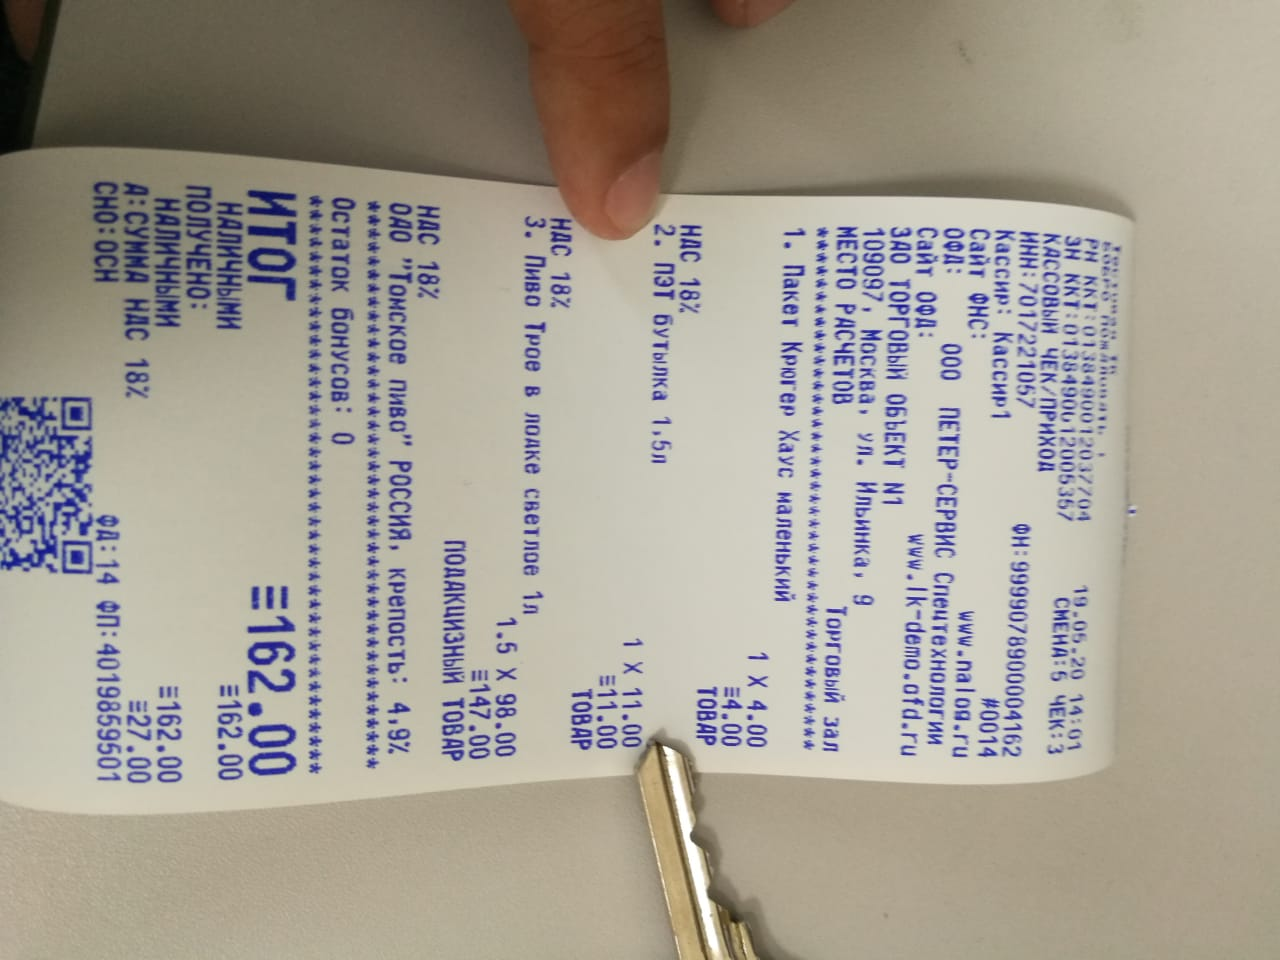
\includegraphics[width=225pt]{2.jpeg}} at (0pt,0pt)
    \end{tikzpicture}
    ;\par
    3. Табличная часть <<Товары>> в форме рабочего места кассира очистится;\par
    4. Поле <<СНО>> в чеке имеет значение <<ОСН>>&  \\
    \hline
    %****************************************************************************************************


   \multicolumn{4}{|c|}{\textbf{\textit{Проверка простого чека с кулинарией}}} \\
   \hline
   \hline
   \Rownum & Запустить конфигурацию магазина выбрав пользователя <<Абрамовская Е. (кассир)>> & 1.Открылся общий интерфейс программы;\par
   2. Отображаются разделы <<Главное>> и <<Продажи>>;\par
   3. Открылась обработка <<Рабочее место кассира>>  &  \\
   \hline
   \Rownum	& Нажать кнопку \keys{Регистрация продаж} в меню РМК & 1. Форма меню РМК закрыта;\par
   2. Открыта форма с информационным сообщением для кассиров;\par
   3. Кнопка \keys{ОК} в нижней части формы недоступна &  \\
   \hline
   \Rownum	& Отметить чек бокс с надписью <<Мною прочитано и понято>> & 1. Чек бокс с надписью <<Мною прочитано и понято>> отмечен ;\par
   2. Кнопка \keys{ОК} в нижней части формы доступна &   \\
   \hline
   \Rownum	& Нажать кнопку \keys{ОК} в нижней части формы & 1. Форма с информационным сообщением для кассиров закрыта.;\par
   2. Открыта форма Рабочего места кассира  &  \\
   \hline
   \Rownum	& Нажать кнопку \keys{Поиск (F11)} в верхней части формы или горячую клавишу \keys{F11} & Открыта форма поиска и подбора товара в РМК &  \\
   \hline
   \Rownum	& Выбрать поиск по наименованию в выпадающем списке <<Поиск>> верхней части формы  & Выбран режим поиска по наименованию &  \\
   \hline
   \Rownum	& В поле поиска ввести <<Гренки чесночные>>  & В табличной части <<Товары>> осталась номенклатура, в наименовании которой содержится <<Гренки чесночные>> &  \\
   \hline
   \Rownum	& В табличной части <<Товары>> выбрать позицию с артикулом <<11432>>  & 1. Форма поиска закрылась;\par
   2. В табличную часть <<Товары>> формы рабочего места кассира добавлена позиция с артикулом <<11432>> с количеством <<1>> и установленной ценой &  \\
   \Rownum	& Установить количество позиции с артикулом <<11432>> равным <<0,150>>  & 1. Количество позиции с артикулом <<11432>> - <<Гренки чесночные>> изменилось на значение <<0,150>>&  \\
   \hline

   \Rownum	& Нажать кнопку \keys{Оплата (F8)} в верхней части формы или горячую клавишу \keys{F8}  &  Открыта форма оплаты &  \\
   \hline
   \Rownum	& Нажать кнопку \keys{Нал.(F6)} справа от поля ввода <<Всего к оплате (руб):>> или горячую клавишу \keys{F6}  & В табличную часть <<Виды оплат>> добавлена строка со значениями полей: <<Вида оплаты>> - <<Наличные>>; <<Сумма>> - рассчитанной суммой&  \\
   \hline
   \Rownum	& Нажать кнопку \keys{Enter} в области цифровых кнопок или горячую клавишу \keys{Ctrl + Enter}  & 1. Форма оплаты закроется;\par
   2. На фискальном регистраторе будет напечатан чек вида:
   \begin{tikzpicture}
   \pgftext{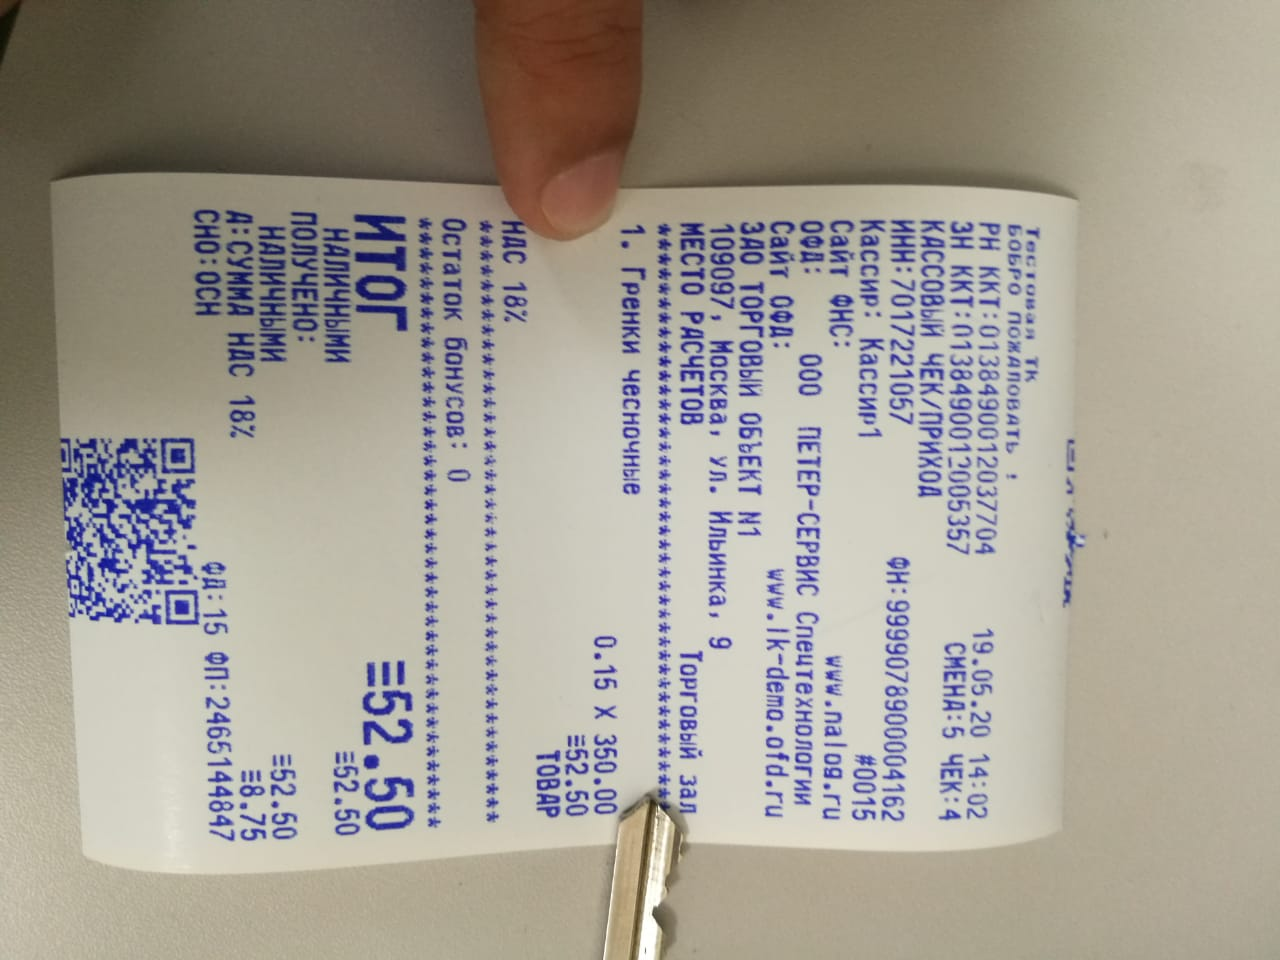
\includegraphics[width=225pt]{3.jpeg}} at (0pt,0pt)
   \end{tikzpicture}
   ;\par
   3. Табличная часть <<Товары>> в форме рабочего места кассира очистится;\par
   4. Поле <<СНО>> в чеке имеет значение <<УСН>>&  \\
   \hline
   %****************************************************************************************************




    \multicolumn{4}{|c|}{\textbf{\textit{Проверка чека с кулинарией и прочим товаром}}} \\
   \hline
   \hline
   \Rownum & Запустить конфигурацию магазина выбрав пользователя <<Абрамовская Е. (кассир)>> & 1.Открылся общий интерфейс программы;\par
   2. Отображаются разделы <<Главное>> и <<Продажи>>;\par
   3. Открылась обработка <<Рабочее место кассира>>  &  \\
   \hline
   \Rownum	& Нажать кнопку \keys{Регистрация продаж} в меню РМК & 1. Форма меню РМК закрыта;\par
   2. Открыта форма с информационным сообщением для кассиров;\par
   3. Кнопка \keys{ОК} в нижней части формы недоступна &  \\
   \hline
   \Rownum	& Отметить чек бокс с надписью <<Мною прочитано и понято>> & 1. Чек бокс с надписью <<Мною прочитано и понято>> отмечен ;\par
   2. Кнопка \keys{ОК} в нижней части формы доступна &   \\
   \hline
   \Rownum	& Нажать кнопку \keys{ОК} в нижней части формы & 1. Форма с информационным сообщением для кассиров закрыта.;\par
   2. Открыта форма Рабочего места кассира  &  \\
   \hline
   \Rownum	& Нажать кнопку \keys{Поиск (F11)} в верхней части формы или горячую клавишу \keys{F11} & Открыта форма поиска и подбора товара в РМК &  \\
   \hline
   \Rownum	& Выбрать поиск по наименованию в выпадающем списке <<Поиск>> верхней части формы  & Выбран режим поиска по наименованию &  \\
   \hline
   \Rownum	& В поле поиска ввести <<Гренки чесночные>>  & В табличной части <<Товары>> осталась номенклатура, в наименовании которой содержится <<Гренки чесночные>> &  \\
   \hline
   \Rownum	& В табличной части <<Товары>> выбрать позицию с артикулом <<11432>>  & 1. Форма поиска закрылась;\par
   2. В табличную часть <<Товары>> формы рабочего места кассира добавлена позиция с артикулом <<11432>> с количеством <<1>> и установленной ценой &  \\
   \Rownum	& Установить количество позиции с артикулом <<11432>> равным <<0,150>>  & 1. Количество позиции с артикулом <<11432>> - <<Гренки чесночные>> изменилось на значение <<0,150>>&  \\
   \hline
    \Rownum	& Нажать кнопку \keys{Поиск (F11)} в верхней части формы или горячую клавишу \keys{F11} & Открыта форма поиска и подбора товара в РМК &  \\
   \hline
   \Rownum	& Выбрать поиск по наименованию в выпадающем списке <<Поиск>> верхней части формы  & Выбран режим поиска по наименованию &  \\
   \hline
   \Rownum	& В поле поиска ввести <<Трое в лодке светлое>>  & В табличной части <<Товары>> осталась номенклатура, в наименовании которой содержится <<Трое в лодке светлое>> &  \\
   \hline
   \Rownum	& В табличной части <<Товары>> выбрать позицию с артикулом <<11697>>  & 1. Форма поиска закрылась;\par
   2. В табличную часть <<Товары>> формы рабочего места кассира добавлена позиция с артикулом <<11697>> с количеством <<1>> и установленной ценой &  \\
   \hline
   \Rownum	& Нажать \keys{Ctrl} + \keys{M}   & 1. В табличную часть <<Товары>> формы рабочего места кассира добавлена позиция с артикулом <<10340>> - <<ПЭТ бутылка 1,5л>>  &  \\
   \hline
   \Rownum	& Установить количество позиции с артикулом <<10340>> равным <<1>>  & 1. Количество позиции с артикулом <<11697>> - <<Пиво Трое в лодке светлое 1л>> изменилось на значение <<1.5>>&  \\
   \hline
   \Rownum	& Нажать кнопку \keys{Оплата (F8)} в верхней части формы или горячую клавишу \keys{F8}  &  Открыта форма оплаты &  \\
   \hline
   \Rownum	& Нажать кнопку \keys{Нал.(F6)} справа от поля ввода <<Всего к оплате (руб):>> или горячую клавишу \keys{F6}  & В табличную часть <<Виды оплат>> добавлена строка со значениями полей: <<Вида оплаты>> - <<Наличные>>; <<Сумма>> - рассчитанной суммой&  \\
   \hline
   \Rownum	& Нажать кнопку \keys{Enter} в области цифровых кнопок или горячую клавишу \keys{Ctrl + Enter}  & 1. Форма оплаты закроется;\par
   2. На фискальном регистраторе будет напечатано два чека. Первый вида:
   \begin{tikzpicture}
   \pgftext{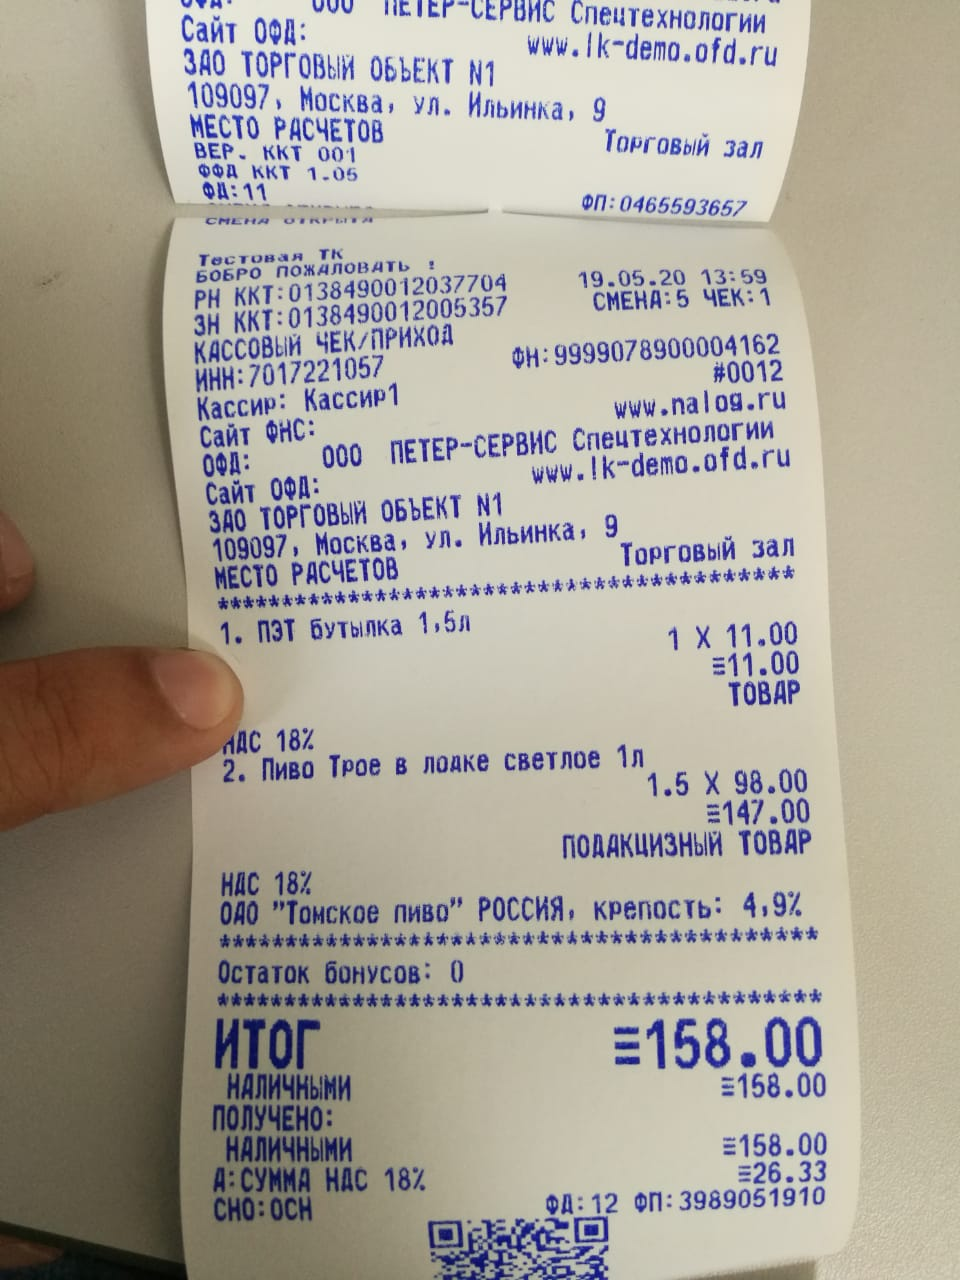
\includegraphics[width=125pt]{1.jpeg}} at (0pt,0pt)
   \end{tikzpicture}
   ;\par
   3. Поле <<СНО>> в чеке имеет значение <<ОСН>>;\par
   4. Второй чек вида:
   \begin{tikzpicture}
   \pgftext{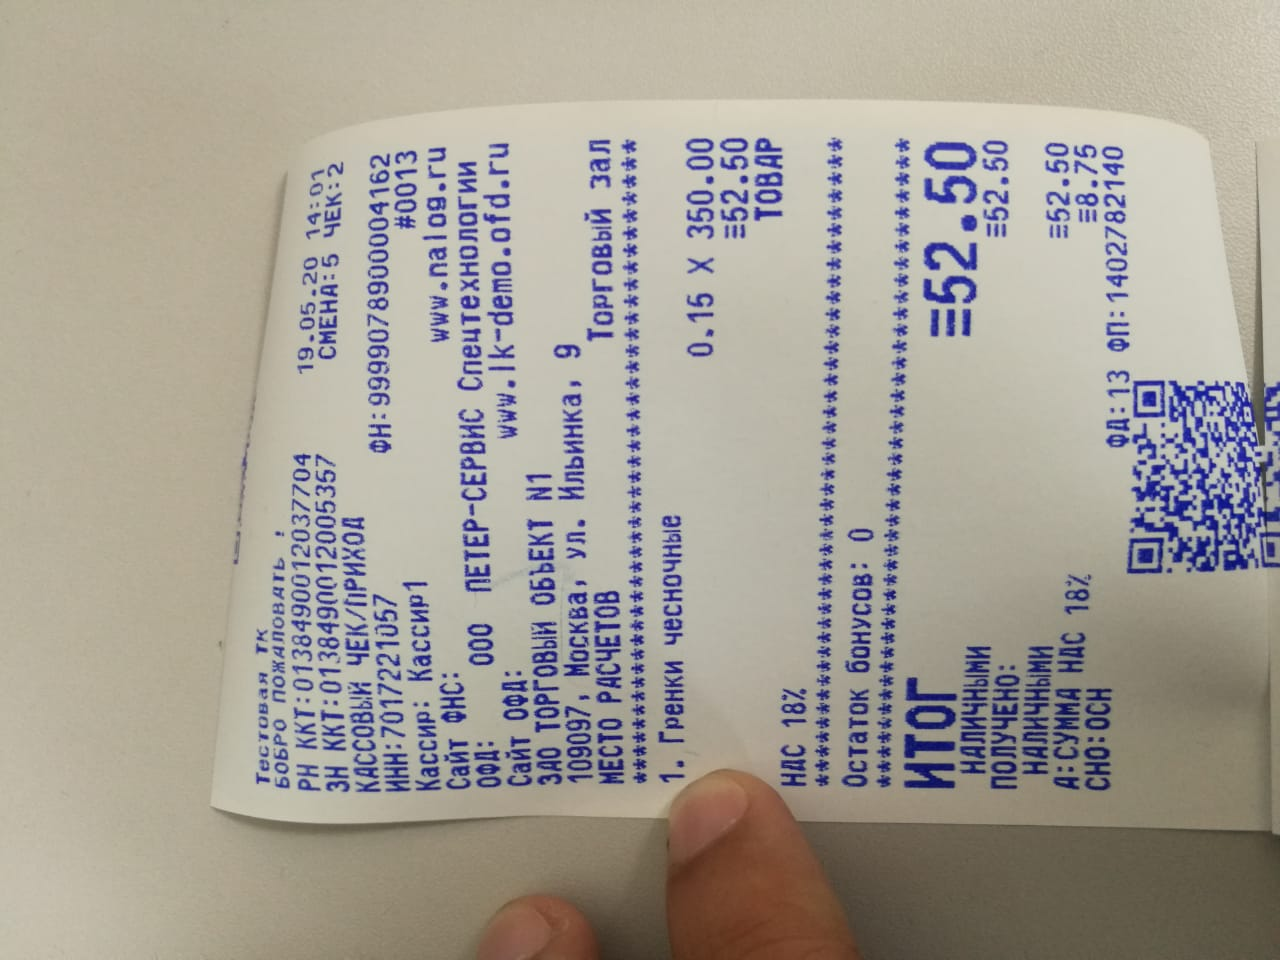
\includegraphics[width=125pt]{4.jpeg}} at (0pt,0pt)
   \end{tikzpicture}
   ;\par
   5. Поле <<СНО>> в чеке имеет значение <<УСН>>;\par
   6. Табличная часть <<Товары>> в форме рабочего места кассира очистится;\par
   &  \\
   \hline
   %****************************************************************************************************


   \multicolumn{4}{|c|}{\textbf{\textit{Проверка блокировки одновременной оплаты по безналичному расчету на разных кассах}}} \\
   \hline
   \hline
   \Rownum &  Проверить, что включена константа «крюВключитьБлокировкуПараллельнойОплатыЭквайринг» включить если не включена & Включена константа «крюВключитьБлокировкуПараллельнойОплатыЭквайринг» &  \\
   \hline
   \Rownum &  Проверить, что включена константа «крюБлокировкаПараллельнойОплатыЭквайринг» включить если не включена & Включена константа «крюБлокировкаПараллельнойОплатыЭквайринг» &
   \\
   \hline
   \Rownum & Запустить конфигурацию магазина выбрав пользователя <<Абрамовская Е. (кассир)>> & 1.Открылся общий интерфейс программы;\par
   2. Отображаются разделы <<Главное>> и <<Продажи>>;\par
   3. Открылась обработка <<Рабочее место кассира>>  &  \\
   \hline
   \Rownum	& Нажать кнопку \keys{Регистрация продаж} в меню РМК & 1. Форма меню РМК закрыта;\par
   2. Открыта форма с информационным сообщением для кассиров;\par
   3. Кнопка \keys{ОК} в нижней части формы недоступна &  \\
   \hline
   \Rownum	& Отметить чек бокс с надписью <<Мною прочитано и понято>> & 1. Чек бокс с надписью <<Мною прочитано и понято>> отмечен ;\par
   2. Кнопка \keys{ОК} в нижней части формы доступна &   \\
   \hline
   \Rownum	& Нажать кнопку \keys{ОК} в нижней части формы & 1. Форма с информационным сообщением для кассиров закрыта.;\par
   2. Открыта форма Рабочего места кассира  &  \\
   \hline
   \Rownum	& Нажать кнопку \keys{Поиск (F11)} в верхней части формы или горячую клавишу \keys{F11} & Открыта форма поиска и подбора товара в РМК &  \\
   \hline
   \Rownum	& Выбрать поиск по наименованию в выпадающем списке <<Поиск>> верхней части формы  & Выбран режим поиска по наименованию &  \\
   \hline
   \Rownum	& В поле поиска ввести <<Гренки чесночные>>  & В табличной части <<Товары>> осталась номенклатура, в наименовании которой содержится <<Гренки чесночные>> &  \\
   \hline
   \Rownum	& В табличной части <<Товары>> выбрать позицию с артикулом <<11432>>  & 1. Форма поиска закрылась;\par
   2. В табличную часть <<Товары>> формы рабочего места кассира добавлена позиция с артикулом <<11432>> с количеством <<1>> и установленной ценой &  \\
   \Rownum	& Установить количество позиции с артикулом <<11432>> равным <<0,150>>  & 1. Количество позиции с артикулом <<11432>> - <<Гренки чесночные>> изменилось на значение <<0,150>>&  \\
   \hline

   \Rownum	& Нажать кнопку \keys{Оплата (F8)} в верхней части формы или горячую клавишу \keys{F8}  &  Открыта форма оплаты &  \\
   \hline
   \Rownum	& Нажать кнопку \keys{Нал.(F6)} справа от поля ввода <<Всего к оплате (руб):>> или горячую клавишу \keys{F6}  & Появляется окно с сообщением <<"Осуществляется оплата по безналу на другой кассе, подождите...">> & !!!!!!!!!  \\
   \hline

   %****************************************************************************************************
\end{longtable}



% РМ
%\begin{longtable}{|p{0.02\linewidth}|p{0.3\linewidth}|p{0.3\linewidth}|p{0.3\linewidth}|}s%
\begin{longtable}{|p{0.02\linewidth}|p{0.3\linewidth}|p{0.3\linewidth}|p{0.3\linewidth}|}
    %  {|c|c|l|c|}
    \hline
    № & \textbf{Действие} & \textbf{Ожидаемый результат} & \textbf{Фактический результат} \\
    %****************************************************************************************************
    \hline
    \hline
    \endhead

    \multicolumn{4}{|c|}{\textbf{\textit{Проверка запуска РМК при старте}}} \\
    \hline
    \Rownum & Запустить конфигурацию магазина  & 1.Открылся общий интерфейс программы;\par
    2. Отображаются все доступные разделы  &  \\
    \hline
    \Rownum & Перейти в раздел <<Администрирование>>   & 1. Открылся отдел <<Администрирование>>
    &  \\

    \hline
    \Rownum	& Выбрать пункт <<Настройки пользователей и прав>>  & Открылся раздел <<Настройки пользователей и прав>>   &  \\
    \hline
    \Rownum	& Выбрать пункт  <<Пользователи>> & Открылся раздел <<Пользователи>> &  \\
    \hline
    \Rownum & В списке пользователей открыть пользователя с именем  <<Абрамовская Екатерина>> & Открылась форма элемента справочника  <<Пользователи>> со значением <<Абрамовская Екатерина>> &  \\
    \hline
    \Rownum	& Перейти в редактирование закладки <<Группы>> & 1. Открылся список групп, в которые включен пользователь;\par
    2. В списке выбранна группа <<Кассиры>>  &  \\
    \hline
    \Rownum	& Снять выбор с группы <<Кассиры>> и установить выбор на группу <<Заведующие магазинами>>  & Снят выбор с группы <<Кассиры>> и установлен выбор на группу <<Заведующие магазинами>>  &  \\
    \hline
    \Rownum	& Нажать кнопку \keys{Записать}  & Изменения сохранились &  \\
    \hline
    \Rownum	& Перейти в редактирование закладки <<Основное>>  & Открылась форма с основными настройками пользователя  &  \\
    \hline
    \Rownum	& Нажать кнопку \keys{Записать и закрыть} & Закрылась форма элемента справочника  <<Пользователи>> со значением <<Абрамовская Екатерина>>  &  \\
    \hline
    \Rownum	& Закрыть конфигурацию  & Конфигурация закрылась  &  \\
    \hline
    \Rownum & Запустить конфигурацию магазина выбрав пользователя <<Абрамовская Е. (кассир)>> & 1.Открылся общий интерфейс программы;\par
    2. Отображаются все доступные разделы;\par
    3. Обработка <<Рабочее место кассира>> не открылась &  \\
    \hline
    \hline
    \Rownum & Перейти в раздел <<Администрирование>>   & 1. Открылся отдел <<Администрирование>>
    &  \\

    \hline
    \Rownum	& Выбрать пункт <<Настройки пользователей и прав>>  & Открылся раздел <<Настройки пользователей и прав>>   &  \\
    \hline
    \Rownum	& Выбрать пункт  <<Пользователи>> & Открылся раздел <<Пользователи>> &  \\
    \hline
    \Rownum & В списке пользователей открыть пользователя с именем  <<Абрамовская Екатерина>> & Открылась форма элемента справочника  <<Пользователи>> со значением <<Абрамовская Екатерина>> &  \\
    \hline
    \Rownum	& Перейти в редактирование закладки <<Группы>> & 1. Открылся список групп, в которые включен пользователь;\par
    2. В списке выбранна группа <<Заведующие магазинами>>  &  \\
    \hline
    \Rownum	& Снять выбор с группы <<Заведующие магазинами>> и установить выбор на группу <<Кассиры>>  & Снят выбор с группы <<Заведующие магазинами>> и установлен выбор на группу <<Кассиры>>  &  \\
    \hline
    \Rownum	& Нажать кнопку \keys{Записать}  & Изменения сохранились &  \\
    \hline
    \Rownum	& Перейти в редактирование закладки <<Основное>>  & Открылась форма с основными настройками пользователя  &  \\
    \hline

    \Rownum	& Нажать кнопку \keys{Записать и закрыть} & Закрылась форма элемента справочника  <<Пользователи>> со значением <<Абрамовская Екатерина>>  &  \\
    \hline
    \Rownum	& Закрыть конфигурацию  & Конфигурация закрылась  &  \\
    \hline
    \Rownum & Запустить конфигурацию магазина выбрав пользователя <<Абрамовская Е. (кассир)>> & 1.Открылся общий интерфейс программы;\par
    2. Отображаются разделы <<Главное>> и <<Продажи>>;\par
    3. Открылась обработка <<Рабочее место кассира>>  &  \\
    \hline
    %****************************************************************************************************

\end{longtable}% РМ
\begin{longtable}{|p{0.02\linewidth}|p{0.3\linewidth}|p{0.3\linewidth}|p{0.3\linewidth}|}
    %  {|c|c|l|c|}
    \hline
    № & \textbf{Действие} & \textbf{Ожидаемый результат} & \textbf{Фактический результат} \\
    %****************************************************************************************************
    \hline
    \hline
    \endhead

   %****************************************************************************************************

    \multicolumn{4}{|c|}{\textbf{\textit{Проверка возможности открытия кассовой смены}}} \\
    \hline
    \hline
    \Rownum & Запустить конфигурацию магазина выбрав пользователя <<Абрамовская Е. (кассир)>> & 1.Открылся общий интерфейс программы;\par
    2. Отображаются разделы <<Главное>> и <<Продажи>>;\par
     3. Открылась обработка <<Рабочее место кассира>>  &  \\
    \hline
     \Rownum	& Нажать кнопку \keys{Открытие смены} в меню РМК & 1. Кассовая смена открыта;\par
     2. На фискальном регистраторе напечатан чек открытия смены &  \\
     \hline
 %****************************************************************************************************

\end{longtable}% РМ
\begin{longtable}{|p{0.02\linewidth}|p{0.3\linewidth}|p{0.3\linewidth}|p{0.3\linewidth}|}
    %  {|c|c|l|c|}
    \hline
    № & \textbf{Действие} & \textbf{Ожидаемый результат} & \textbf{Фактический результат} \\
    %****************************************************************************************************
    \hline
    \hline
    \endhead

   %****************************************************************************************************

  \multicolumn{4}{|c|}{\textbf{\textit{Изменена основная форма РМК, уменьшен размер}}} \\
  \hline
  \hline
  \Rownum & Запустить конфигурацию магазина выбрав пользователя <<Абрамовская Е. (кассир)>> & 1.Открылся общий интерфейс программы;\par
  2. Отображаются разделы <<Главное>> и <<Продажи>>;\par
  3. Открылась обработка <<Рабочее место кассира>>  &  \\

  \hline
  \Rownum	& Нажать кнопку \keys{Регистрация продаж} в меню РМК & 1. Форма меню РМК закрыта;\par
  2. Открыта форма с информационным сообщением для кассиров;\par
  3. Кнопка \keys{ОК} в нижней части формы недоступна &  \\
  \hline
  \Rownum	& Отметить чек бокс с надписью <<Мною прочитано и понято>> & 1. Чек бокс с надписью <<Мною прочитано и понято>> отмечен ;\par
  2. Кнопка \keys{ОК} в нижней части формы доступна &   \\
  \hline
  \Rownum	& Нажать кнопку \keys{ОК} в нижней части формы & 1. Форма с информационным сообщением для кассиров закрыта.;\par
  2. Открыта форма Рабочего места кассира;\par
  3. Форма имеет корректные размеры и вмещается на экран без вертикальных и горизонтальных полос прокрутки  &  \\
  \hline
  \Rownum & Закрыть рабочее место кассира нажав последовательно горячие клавиши \keys{F10} - \keys{F12}  & Открылось меню <<Рабочего места кассира>>;\par
  &  \\
  \hline
  \Rownum & Нажать кнопку \keys{Завершение работы}   & Конфигурация закрылась
  &  \\
  \hline
  %****************************************************************************************************

\end{longtable}% РМ
\begin{longtable}{|p{0.02\linewidth}|p{0.3\linewidth}|p{0.3\linewidth}|p{0.3\linewidth}|}
    %  {|c|c|l|c|}
    \hline
    № & \textbf{Действие} & \textbf{Ожидаемый результат} & \textbf{Фактический результат} \\
    %****************************************************************************************************
    \hline
    \hline
    \endhead

   %****************************************************************************************************

 \multicolumn{4}{|c|}{\textbf{\textit{Проверка различных алгоритмов и элементов формы}}} \\
 \hline
 \hline
 \Rownum & Запустить конфигурацию магазина выбрав пользователя <<Абрамовская Е. (кассир)>> & 1.Открылся общий интерфейс программы;\par
 2. Отображаются разделы <<Главное>> и <<Продажи>>;\par
 3. Открылась обработка <<Рабочее место кассира>>  &  \\
 \hline
 \Rownum	& Нажать кнопку \keys{Регистрация продаж} в меню РМК & 1. Форма меню РМК закрыта;\par
 2. Открыта форма с информационным сообщением для кассиров;\par
 3. Кнопка \keys{ОК} в нижней части формы недоступна &  \\
 \hline
 \Rownum	& Отметить чек бокс с надписью <<Мною прочитано и понято>> & 1. Чек бокс с надписью <<Мною прочитано и понято>> отмечен ;\par
 2. Кнопка \keys{ОК} в нижней части формы доступна &   \\
 \hline
 \Rownum	& Нажать кнопку \keys{ОК} в нижней части формы & 1. Форма с информационным сообщением для кассиров закрыта.;\par
 2. Открыта форма Рабочего места кассира  &  \\
 \hline
 \Rownum	& Проверить кнопки в верхней части формы & Присутствуют кнопки:\par 1. <<Меню>>;\par
 2. <<Поиск>>;\par
 3. <<Ред.строки>>;\par
 4. <<Возврат>>;\par
 5. <<Бонусы>>;\par
 6. <<Оплата>>;\par
 7. <<Проверить чеки ККМ>> &  \\
 \hline
 \Rownum	& Проверить наличие надписи <<ОстатокБонусов>> & 1. Присутствует надпись <<Остаток бонусов на карте>>;\par
 2. Справа от надписи поле ввода со значением <<0>>;\par
 3. Справа от поля ввода кнопка <<Обновить состояния дисконтного сервера>> &  \\
 \hline
 \Rownum	& Проверить состав полей в табличной части <<Товары>> & Присутствуют только поля:\par
 1. <<Артикул>>;\par
 2. <<Номенклатура>>;\par
 3. <<Количество>>;\par
 4. <<Цена>>;\par
 5. <<Сумма>> &  \\
 \hline
 \Rownum	& Нажать кнопку \keys{Поиск (F11)} в верхней части формы или горячую клавишу \keys{F11} & Открыта форма поиска и подбора товара в РМК &  \\
 \hline
 \Rownum	& Нажать на текстовую метку <<Показать информацию>> в нижней части формы  & 1. В нижней части формы отображается табличная часть;\par
 2. Под табличной частью чек бокс <<остатки>> недоступен для редактирования &  \\
 \hline
 %****************************************************************************************************

\end{longtable}% РМ
\begin{longtable}{|p{0.02\linewidth}|p{0.3\linewidth}|p{0.3\linewidth}|p{0.3\linewidth}|}
    %  {|c|c|l|c|}
    \hline
    № & \textbf{Действие} & \textbf{Ожидаемый результат} & \textbf{Фактический результат} \\
    %****************************************************************************************************
    \hline
    \hline
    \endhead

   %****************************************************************************************************

    \multicolumn{4}{|c|}{\textbf{\textit{Проверка автоматического подбора количества разливного пива при выборе тары}}} \\
\hline
\hline
\Rownum & Запустить конфигурацию магазина выбрав пользователя <<Абрамовская Е. (кассир)>> & 1.Открылся общий интерфейс программы;\par
2. Отображаются разделы <<Главное>> и <<Продажи>>;\par
3. Открылась обработка <<Рабочее место кассира>>  &  \\
\hline
\Rownum	& Нажать кнопку \keys{Регистрация продаж} в меню РМК & 1. Форма меню РМК закрыта;\par
2. Открыта форма с информационным сообщением для кассиров;\par
3. Кнопка \keys{ОК} в нижней части формы недоступна &  \\
\hline
\Rownum	& Отметить чек бокс с надписью <<Мною прочитано и понято>> & 1. Чек бокс с надписью <<Мною прочитано и понято>> отмечен ;\par
2. Кнопка \keys{ОК} в нижней части формы доступна &   \\
\hline
\Rownum	& Нажать кнопку \keys{ОК} в нижней части формы & 1. Форма с информационным сообщением для кассиров закрыта.;\par
2. Открыта форма Рабочего места кассира  &  \\
\hline
\Rownum	& Нажать кнопку \keys{Поиск (F11)} в верхней части формы или горячую клавишу \keys{F11} & Открыта форма поиска и подбора товара в РМК &  \\
\hline
\Rownum	& Выбрать поиск по наименованию в выпадающем списке <<Поиск>> верхней части формы  & Выбран режим поиска по наименованию &  \\
\hline
\Rownum	& В поле поиска ввести <<Трое в лодке светлое>>  & В табличной части <<Товары>> осталась номенклатура, в наименовании которой содержится <<Трое в лодке светлое>> &  \\
\hline
\Rownum	& В табличной части <<Товары>> выбрать позицию с артикулом <<11697>>  & 1. Форма поиска закрылась;\par
2. В табличную часть <<Товары>> формы рабочего места кассира добавлена позиция с артикулом <<11697>> с количеством <<1>> и установленной ценой &  \\
\hline
\Rownum	& Нажать \keys{Ctrl} + \keys{M}   & 1. В табличную часть <<Товары>> формы рабочего места кассира добавлена позиция с артикулом <<10340>> - <<ПЭТ бутылка 1,5л>>  &  \\
\hline
\Rownum	& Установить количество позиции с артикулом <<10340>> равным <<2>>  & 1. Количество позиции с артикулом <<11697>> - <<Пиво Трое в лодке светлое 1л>> изменилось на значение <<3>>&  \\
\hline
%****************************************************************************************************

\end{longtable}% РМ
\begin{longtable}{|p{0.02\linewidth}|p{0.3\linewidth}|p{0.3\linewidth}|p{0.3\linewidth}|}
    %  {|c|c|l|c|}
    \hline
    № & \textbf{Действие} & \textbf{Ожидаемый результат} & \textbf{Фактический результат} \\
    %****************************************************************************************************
    \hline
    \hline
    \endhead

   %****************************************************************************************************

    \multicolumn{4}{|c|}{\textbf{\textit{Проверка запрета продажи разливного товара без тары}}} \\
\hline
\hline
\Rownum & Запустить конфигурацию магазина выбрав пользователя <<Абрамовская Е. (кассир)>> & 1.Открылся общий интерфейс программы;\par
2. Отображаются разделы <<Главное>> и <<Продажи>>;\par
3. Открылась обработка <<Рабочее место кассира>>  &  \\
\hline
\Rownum	& Нажать кнопку \keys{Регистрация продаж} в меню РМК & 1. Форма меню РМК закрыта;\par
2. Открыта форма с информационным сообщением для кассиров;\par
3. Кнопка \keys{ОК} в нижней части формы недоступна &  \\
\hline
\Rownum	& Отметить чек бокс с надписью <<Мною прочитано и понято>> & 1. Чек бокс с надписью <<Мною прочитано и понято>> отмечен ;\par
2. Кнопка \keys{ОК} в нижней части формы доступна &   \\
\hline
\Rownum	& Нажать кнопку \keys{ОК} в нижней части формы & 1. Форма с информационным сообщением для кассиров закрыта.;\par
2. Открыта форма Рабочего места кассира  &  \\
\hline
\Rownum	& Нажать кнопку \keys{Поиск (F11)} в верхней части формы или горячую клавишу \keys{F11} & Открыта форма поиска и подбора товара в РМК &  \\
\hline
\Rownum	& Выбрать поиск по наименованию в выпадающем списке <<Поиск>> верхней части формы  & Выбран режим поиска по наименованию &  \\
\hline
\Rownum	& В поле поиска ввести <<Трое в лодке светлое>>  & В табличной части <<Товары>> осталась номенклатура, в наименовании которой содержится <<Трое в лодке светлое>> &  \\
\hline
\Rownum	& В табличной части <<Товары>> выбрать позицию с артикулом <<11697>>  & 1. Форма поиска закрылась;\par
2. В табличную часть <<Товары>> формы рабочего места кассира добавлена позиция с артикулом <<11697>> с количеством <<1>> и установленной ценой &  \\
\hline
\Rownum	& Нажать кнопку \keys{Оплата (F8)} в верхней части формы или горячую клавишу \keys{F8}  & Открыта форма с информационным сообщением << Внимание! Объём тары и объём разливных напитков расходятся на -1л. !>>  &  \\
\hline

%****************************************************************************************************

\end{longtable}% Проверка запрета продажи разливного товара без тары
\begin{longtable}{|p{0.02\linewidth}|p{0.3\linewidth}|p{0.3\linewidth}|p{0.3\linewidth}|}
    %  {|c|c|l|c|}
    \hline
    № & \textbf{Действие} & \textbf{Ожидаемый результат} & \textbf{Фактический результат} \\
    %****************************************************************************************************
    \hline
    \hline
    \endhead

   %****************************************************************************************************

     \multicolumn{4}{|c|}{\textbf{\textit{Проверка сообщения о превышении количества}}} \\
\hline
\hline
\Rownum & Запустить конфигурацию магазина выбрав пользователя <<Абрамовская Е. (кассир)>> & 1.Открылся общий интерфейс программы;\par
2. Отображаются разделы <<Главное>> и <<Продажи>>;\par
3. Открылась обработка <<Рабочее место кассира>>  &  \\
\hline
\Rownum	& Нажать кнопку \keys{Регистрация продаж} в меню РМК & 1. Форма меню РМК закрыта;\par
2. Открыта форма с информационным сообщением для кассиров;\par
3. Кнопка \keys{ОК} в нижней части формы недоступна &  \\
\hline
\Rownum	& Отметить чек бокс с надписью <<Мною прочитано и понято>> & 1. Чек бокс с надписью <<Мною прочитано и понято>> отмечен ;\par
2. Кнопка \keys{ОК} в нижней части формы доступна &   \\
\hline
\Rownum	& Нажать кнопку \keys{ОК} в нижней части формы & 1. Форма с информационным сообщением для кассиров закрыта.;\par
2. Открыта форма Рабочего места кассира  &  \\
\hline
\Rownum	& Нажать кнопку \keys{Поиск (F11)} в верхней части формы или горячую клавишу \keys{F11} & Открыта форма поиска и подбора товара в РМК &  \\
\hline
\Rownum	& Выбрать поиск по наименованию в выпадающем списке <<Поиск>> верхней части формы  & Выбран режим поиска по наименованию &  \\
\hline
\Rownum	& В поле поиска ввести <<Трое в лодке светлое>>  & В табличной части <<Товары>> осталась номенклатура, в наименовании которой содержится <<Трое в лодке светлое>> &  \\
\hline
\Rownum	& В табличной части <<Товары>> выбрать позицию с артикулом <<11697>>  & 1. Форма поиска закрылась;\par
2. В табличную часть <<Товары>> формы рабочего места кассира добавлена позиция с артикулом <<11697>> с количеством <<1>> и установленной ценой &  \\
\hline

\Rownum	& Нажать \keys{Ctrl} + \keys{M}   & 1. В табличную часть <<Товары>> формы рабочего места кассира добавлена позиция с артикулом <<10340>> - <<ПЭТ бутылка 1,5л>>  &  \\
\hline
\Rownum	& Установить количество позиции с артикулом <<10340>> равным <<20 000>>  & 1. Количество позиции с артикулом <<11697>> - <<Пиво Трое в лодке светлое 1л>> изменилось на значение <<30 000>>&  \\
\hline
\Rownum	& Нажать кнопку \keys{Оплата (F8)} в верхней части формы или горячую клавишу \keys{F8}  & 1. Открыта форма с информационным сообщением << Отрицательные остатки  ПЭТ бутылка 1,5л
Превышен остаток на складе  <<указан склад>>
Пиво Трое в лодке светлое 1л
Превышен остаток на складе <<указан склад>> !>>;\par
2. Количество на сколько превышен остаток не указано  &  \\
\hline
%****************************************************************************************************

\end{longtable}% Проверка сообщения о превышении количества
\begin{longtable}{|p{0.02\linewidth}|p{0.3\linewidth}|p{0.3\linewidth}|p{0.3\linewidth}|}
    %  {|c|c|l|c|}
    \hline
    № & \textbf{Действие} & \textbf{Ожидаемый результат} & \textbf{Фактический результат} \\
    %****************************************************************************************************
    \hline
    \hline
    \endhead

   %****************************************************************************************************

      \multicolumn{4}{|c|}{\textbf{\textit{Проверка различных алгоритмов и элементов формы оплаты}}} \\
\hline
\hline
\Rownum & Запустить конфигурацию магазина выбрав пользователя <<Абрамовская Е. (кассир)>> & 1.Открылся общий интерфейс программы;\par
2. Отображаются разделы <<Главное>> и <<Продажи>>;\par
3. Открылась обработка <<Рабочее место кассира>>  &  \\
\hline
\Rownum	& Нажать кнопку \keys{Регистрация продаж} в меню РМК & 1. Форма меню РМК закрыта;\par
2. Открыта форма с информационным сообщением для кассиров;\par
3. Кнопка \keys{ОК} в нижней части формы недоступна &  \\
\hline
\Rownum	& Отметить чек бокс с надписью <<Мною прочитано и понято>> & 1. Чек бокс с надписью <<Мною прочитано и понято>> отмечен ;\par
2. Кнопка \keys{ОК} в нижней части формы доступна &   \\
\hline
\Rownum	& Нажать кнопку \keys{ОК} в нижней части формы & 1. Форма с информационным сообщением для кассиров закрыта.;\par
2. Открыта форма Рабочего места кассира  &  \\
\hline
\Rownum	& Нажать кнопку \keys{Поиск (F11)} в верхней части формы или горячую клавишу \keys{F11} & Открыта форма поиска и подбора товара в РМК &  \\
\hline
\Rownum	& Выбрать поиск по наименованию в выпадающем списке <<Поиск>> верхней части формы  & Выбран режим поиска по наименованию &  \\
\hline
\Rownum	& В поле поиска ввести <<Трое в лодке светлое>>  & В табличной части <<Товары>> осталась номенклатура, в наименовании которой содержится <<Трое в лодке светлое>> &  \\
\hline
\Rownum	& В табличной части <<Товары>> выбрать позицию с артикулом <<11697>>  & 1. Форма поиска закрылась;\par
2. В табличную часть <<Товары>> формы рабочего места кассира добавлена позиция с артикулом <<11697>> с количеством <<1>> и установленной ценой &  \\
\hline

\Rownum	& Нажать \keys{Ctrl} + \keys{M}   & 1. В табличную часть <<Товары>> формы рабочего места кассира добавлена позиция с артикулом <<10340>> - <<ПЭТ бутылка 1,5л>>  &  \\
\hline
\Rownum	& Установить количество позиции с артикулом <<10340>> равным <<1>>  & 1. Количество позиции с артикулом <<11697>> - <<Пиво Трое в лодке светлое 1л>> изменилось на значение <<1.5>>&  \\
\hline
\Rownum	& Нажать кнопку \keys{Оплата (F8)} в верхней части формы или горячую клавишу \keys{F8}  & 1. Открыта форма оплаты товара  &  \\
\hline

\Rownum& Проверить кнопки справа от поля <<Всего к оплате (руб):>> & Присутствуют только кнопки:\par 1.  <<Нал.(F6)>>;\par
2. <<ПК(F7)>> &  \\
\hline

\Rownum& Проверить кнопки справа от поля <<Остаток (руб):>> & Присутствуют только кнопки:\par 1. <<Послать чек электронным письмом (Ctrl+C)>>;\par
2. <<Послать чек SMS (Ctrl+S)>> &  \\
\hline
%****************************************************************************************************


\end{longtable}% Проверка различных алгоритмов и элементов формы оплаты
\begin{longtable}{|p{0.02\linewidth}|p{0.3\linewidth}|p{0.3\linewidth}|p{0.3\linewidth}|}
    %  {|c|c|l|c|}
    \hline
    № & \textbf{Действие} & \textbf{Ожидаемый результат} & \textbf{Фактический результат} \\
    %****************************************************************************************************
    \hline
    \hline
    \endhead

   %****************************************************************************************************

     \multicolumn{4}{|c|}{\textbf{\textit{Проверка простого чека с алкоголем}}} \\
\hline
\hline
\Rownum & Запустить конфигурацию магазина выбрав пользователя <<Абрамовская Е. (кассир)>> & 1.Открылся общий интерфейс программы;\par
2. Отображаются разделы <<Главное>> и <<Продажи>>;\par
3. Открылась обработка <<Рабочее место кассира>>  &  \\
\hline
\Rownum	& Нажать кнопку \keys{Регистрация продаж} в меню РМК & 1. Форма меню РМК закрыта;\par
2. Открыта форма с информационным сообщением для кассиров;\par
3. Кнопка \keys{ОК} в нижней части формы недоступна &  \\
\hline
\Rownum	& Отметить чек бокс с надписью <<Мною прочитано и понято>> & 1. Чек бокс с надписью <<Мною прочитано и понято>> отмечен ;\par
2. Кнопка \keys{ОК} в нижней части формы доступна &   \\
\hline
\Rownum	& Нажать кнопку \keys{ОК} в нижней части формы & 1. Форма с информационным сообщением для кассиров закрыта.;\par
2. Открыта форма Рабочего места кассира  &  \\
\hline
\Rownum	& Нажать кнопку \keys{Поиск (F11)} в верхней части формы или горячую клавишу \keys{F11} & Открыта форма поиска и подбора товара в РМК &  \\
\hline
\Rownum	& Выбрать поиск по наименованию в выпадающем списке <<Поиск>> верхней части формы  & Выбран режим поиска по наименованию &  \\
\hline
\Rownum	& В поле поиска ввести <<Трое в лодке светлое>>  & В табличной части <<Товары>> осталась номенклатура, в наименовании которой содержится <<Трое в лодке светлое>> &  \\
\hline
\Rownum	& В табличной части <<Товары>> выбрать позицию с артикулом <<11697>>  & 1. Форма поиска закрылась;\par
2. В табличную часть <<Товары>> формы рабочего места кассира добавлена позиция с артикулом <<11697>> с количеством <<1>> и установленной ценой &  \\
\hline
\Rownum	& Нажать кнопку \keys{Поиск (F11)} в верхней части формы или горячую клавишу \keys{F11} & Открыта форма поиска и подбора товара в РМК &  \\
\hline
\Rownum	& Выбрать поиск по наименованию в выпадающем списке <<Поиск>> верхней части формы  & Выбран режим поиска по наименованию &  \\
\hline
\Rownum	& В поле поиска ввести <<Пакет Крюгер Хаус маленький>>  & В табличной части <<Товары>> осталась номенклатура, в наименовании которой содержится <<Пакет Крюгер Хаус маленький>> &  \\
\hline
\Rownum	& В табличной части <<Товары>> выбрать позицию с артикулом <<10347>>  & 1. Форма поиска закрылась;\par
2. В табличную часть <<Товары>> формы рабочего места кассира добавлена позиция с артикулом <<10347>> с количеством <<1>> и установленной ценой &  \\
\hline
\Rownum	& Нажать \keys{Ctrl} + \keys{M}   & 1. В табличную часть <<Товары>> формы рабочего места кассира добавлена позиция с артикулом <<10340>> - <<ПЭТ бутылка 1,5л>>  &  \\
\hline
\Rownum	& Установить количество позиции с артикулом <<10340>> равным <<1>>  & 1. Количество позиции с артикулом <<11697>> - <<Пиво Трое в лодке светлое 1л>> изменилось на значение <<1.5>>&  \\
\hline
\Rownum	& Нажать кнопку \keys{Оплата (F8)} в верхней части формы или горячую клавишу \keys{F8}  &  Открыта форма оплаты &  \\
\hline
\Rownum	& Нажать кнопку \keys{Нал.(F6)} справа от поля ввода <<Всего к оплате (руб):>> или горячую клавишу \keys{F6}  & В табличную часть <<Виды оплат>> добавлена строка со значениями полей: <<Вида оплаты>> - <<Наличные>>; <<Сумма>> - рассчитанной суммой&  \\
\hline
\Rownum	& Нажать кнопку \keys{Enter} в области цифровых кнопок или горячую клавишу \keys{Ctrl + Enter}  & 1. Форма оплаты закроется;\par
2. На фискальном регистраторе будет напечатан чек вида:
\begin{tikzpicture}
\pgftext{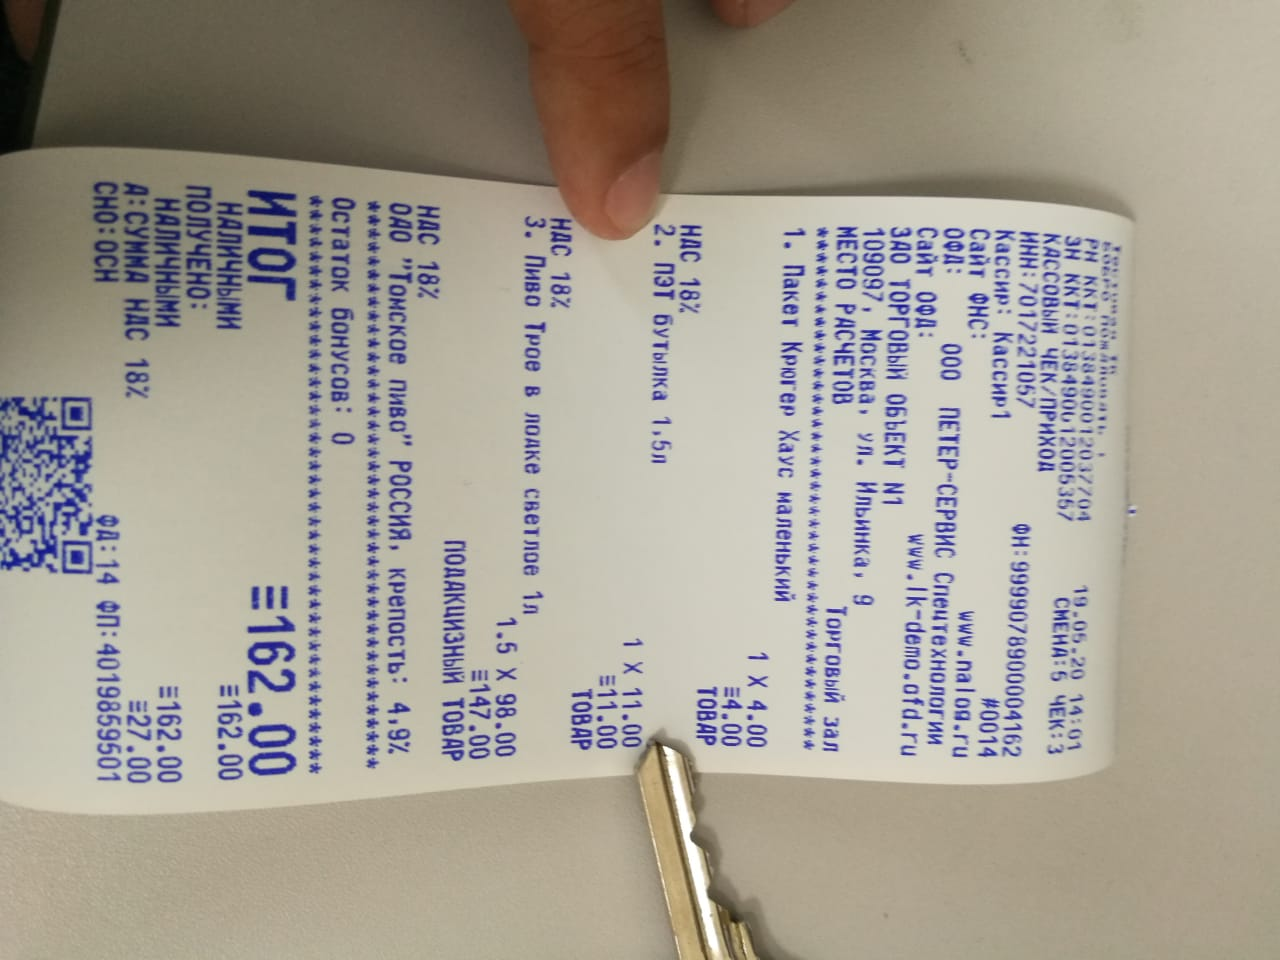
\includegraphics[width=225pt]{2.jpeg}} at (0pt,0pt)
\end{tikzpicture}
;\par
3. Табличная часть <<Товары>> в форме рабочего места кассира очистится;\par
4. Поле <<СНО>> в чеке имеет значение <<ОСН>>&  \\
\hline
%****************************************************************************************************


\end{longtable}% Проверка простого чека с алкоголем
\begin{longtable}{|p{0.02\linewidth}|p{0.3\linewidth}|p{0.3\linewidth}|p{0.3\linewidth}|}
    %  {|c|c|l|c|}
    \hline
    № & \textbf{Действие} & \textbf{Ожидаемый результат} & \textbf{Фактический результат} \\
    %****************************************************************************************************
    \hline
    \hline
    \endhead

   %****************************************************************************************************

   \multicolumn{4}{|c|}{\textbf{\textit{Проверка простого чека с кулинарией}}} \\
\hline
\hline
\Rownum & Запустить конфигурацию магазина выбрав пользователя <<Абрамовская Е. (кассир)>> & 1.Открылся общий интерфейс программы;\par
2. Отображаются разделы <<Главное>> и <<Продажи>>;\par
3. Открылась обработка <<Рабочее место кассира>>  &  \\
\hline
\Rownum	& Нажать кнопку \keys{Регистрация продаж} в меню РМК & 1. Форма меню РМК закрыта;\par
2. Открыта форма с информационным сообщением для кассиров;\par
3. Кнопка \keys{ОК} в нижней части формы недоступна &  \\
\hline
\Rownum	& Отметить чек бокс с надписью <<Мною прочитано и понято>> & 1. Чек бокс с надписью <<Мною прочитано и понято>> отмечен ;\par
2. Кнопка \keys{ОК} в нижней части формы доступна &   \\
\hline
\Rownum	& Нажать кнопку \keys{ОК} в нижней части формы & 1. Форма с информационным сообщением для кассиров закрыта.;\par
2. Открыта форма Рабочего места кассира  &  \\
\hline
\Rownum	& Нажать кнопку \keys{Поиск (F11)} в верхней части формы или горячую клавишу \keys{F11} & Открыта форма поиска и подбора товара в РМК &  \\
\hline
\Rownum	& Выбрать поиск по наименованию в выпадающем списке <<Поиск>> верхней части формы  & Выбран режим поиска по наименованию &  \\
\hline
\Rownum	& В поле поиска ввести <<Гренки чесночные>>  & В табличной части <<Товары>> осталась номенклатура, в наименовании которой содержится <<Гренки чесночные>> &  \\
\hline
\Rownum	& В табличной части <<Товары>> выбрать позицию с артикулом <<11432>>  & 1. Форма поиска закрылась;\par
2. В табличную часть <<Товары>> формы рабочего места кассира добавлена позиция с артикулом <<11432>> с количеством <<1>> и установленной ценой &  \\
\Rownum	& Установить количество позиции с артикулом <<11432>> равным <<0,150>>  & 1. Количество позиции с артикулом <<11432>> - <<Гренки чесночные>> изменилось на значение <<0,150>>&  \\
\hline

\Rownum	& Нажать кнопку \keys{Оплата (F8)} в верхней части формы или горячую клавишу \keys{F8}  &  Открыта форма оплаты &  \\
\hline
\Rownum	& Нажать кнопку \keys{Нал.(F6)} справа от поля ввода <<Всего к оплате (руб):>> или горячую клавишу \keys{F6}  & В табличную часть <<Виды оплат>> добавлена строка со значениями полей: <<Вида оплаты>> - <<Наличные>>; <<Сумма>> - рассчитанной суммой&  \\
\hline
\Rownum	& Нажать кнопку \keys{Enter} в области цифровых кнопок или горячую клавишу \keys{Ctrl + Enter}  & 1. Форма оплаты закроется;\par
2. На фискальном регистраторе будет напечатан чек вида:
\begin{tikzpicture}
\pgftext{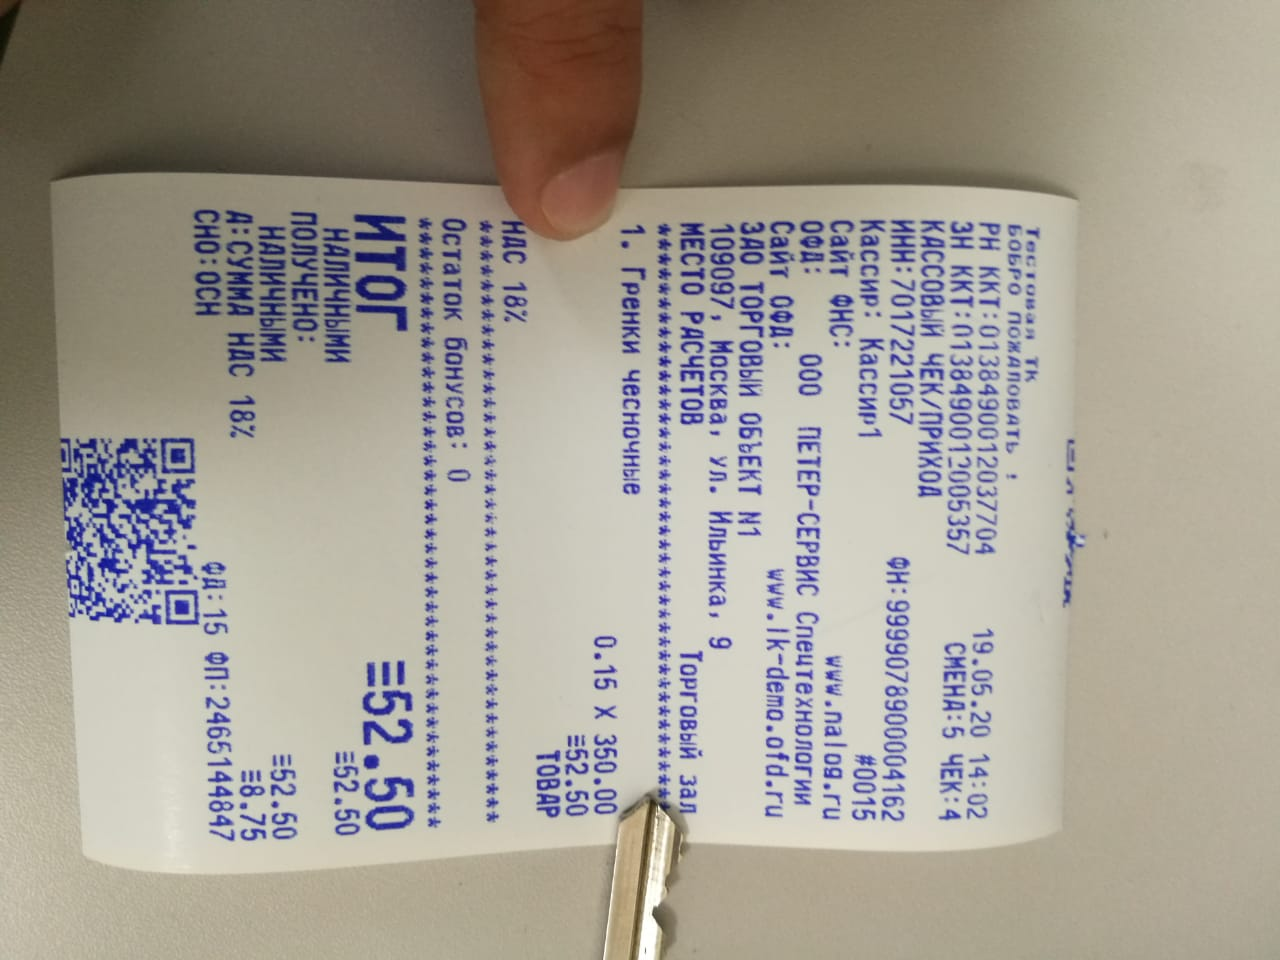
\includegraphics[width=225pt]{3.jpeg}} at (0pt,0pt)
\end{tikzpicture}
;\par
3. Табличная часть <<Товары>> в форме рабочего места кассира очистится;\par
4. Поле <<СНО>> в чеке имеет значение <<УСН>>&  \\
\hline
%****************************************************************************************************



\end{longtable}% Проверка простого чека с кулинарией
\begin{longtable}{|p{0.02\linewidth}|p{0.3\linewidth}|p{0.3\linewidth}|p{0.3\linewidth}|}
    %  {|c|c|l|c|}
    \hline
    № & \textbf{Действие} & \textbf{Ожидаемый результат} & \textbf{Фактический результат} \\
    %****************************************************************************************************
    \hline
    \hline
    \endhead

   %****************************************************************************************************

    \multicolumn{4}{|c|}{\textbf{\textit{Проверка чека с кулинарией и прочим товаром}}} \\
\hline
\hline
\Rownum & Запустить конфигурацию магазина выбрав пользователя <<Абрамовская Е. (кассир)>> & 1.Открылся общий интерфейс программы;\par
2. Отображаются разделы <<Главное>> и <<Продажи>>;\par
3. Открылась обработка <<Рабочее место кассира>>  &  \\
\hline
\Rownum	& Нажать кнопку \keys{Регистрация продаж} в меню РМК & 1. Форма меню РМК закрыта;\par
2. Открыта форма с информационным сообщением для кассиров;\par
3. Кнопка \keys{ОК} в нижней части формы недоступна &  \\
\hline
\Rownum	& Отметить чек бокс с надписью <<Мною прочитано и понято>> & 1. Чек бокс с надписью <<Мною прочитано и понято>> отмечен ;\par
2. Кнопка \keys{ОК} в нижней части формы доступна &   \\
\hline
\Rownum	& Нажать кнопку \keys{ОК} в нижней части формы & 1. Форма с информационным сообщением для кассиров закрыта.;\par
2. Открыта форма Рабочего места кассира  &  \\
\hline
\Rownum	& Нажать кнопку \keys{Поиск (F11)} в верхней части формы или горячую клавишу \keys{F11} & Открыта форма поиска и подбора товара в РМК &  \\
\hline
\Rownum	& Выбрать поиск по наименованию в выпадающем списке <<Поиск>> верхней части формы  & Выбран режим поиска по наименованию &  \\
\hline
\Rownum	& В поле поиска ввести <<Гренки чесночные>>  & В табличной части <<Товары>> осталась номенклатура, в наименовании которой содержится <<Гренки чесночные>> &  \\
\hline
\Rownum	& В табличной части <<Товары>> выбрать позицию с артикулом <<11432>>  & 1. Форма поиска закрылась;\par
2. В табличную часть <<Товары>> формы рабочего места кассира добавлена позиция с артикулом <<11432>> с количеством <<1>> и установленной ценой &  \\
\Rownum	& Установить количество позиции с артикулом <<11432>> равным <<0,150>>  & 1. Количество позиции с артикулом <<11432>> - <<Гренки чесночные>> изменилось на значение <<0,150>>&  \\
\hline
\Rownum	& Нажать кнопку \keys{Поиск (F11)} в верхней части формы или горячую клавишу \keys{F11} & Открыта форма поиска и подбора товара в РМК &  \\
\hline
\Rownum	& Выбрать поиск по наименованию в выпадающем списке <<Поиск>> верхней части формы  & Выбран режим поиска по наименованию &  \\
\hline
\Rownum	& В поле поиска ввести <<Трое в лодке светлое>>  & В табличной части <<Товары>> осталась номенклатура, в наименовании которой содержится <<Трое в лодке светлое>> &  \\
\hline
\Rownum	& В табличной части <<Товары>> выбрать позицию с артикулом <<11697>>  & 1. Форма поиска закрылась;\par
2. В табличную часть <<Товары>> формы рабочего места кассира добавлена позиция с артикулом <<11697>> с количеством <<1>> и установленной ценой &  \\
\hline
\Rownum	& Нажать \keys{Ctrl} + \keys{M}   & 1. В табличную часть <<Товары>> формы рабочего места кассира добавлена позиция с артикулом <<10340>> - <<ПЭТ бутылка 1,5л>>  &  \\
\hline
\Rownum	& Установить количество позиции с артикулом <<10340>> равным <<1>>  & 1. Количество позиции с артикулом <<11697>> - <<Пиво Трое в лодке светлое 1л>> изменилось на значение <<1.5>>&  \\
\hline
\Rownum	& Нажать кнопку \keys{Оплата (F8)} в верхней части формы или горячую клавишу \keys{F8}  &  Открыта форма оплаты &  \\
\hline
\Rownum	& Нажать кнопку \keys{Нал.(F6)} справа от поля ввода <<Всего к оплате (руб):>> или горячую клавишу \keys{F6}  & В табличную часть <<Виды оплат>> добавлена строка со значениями полей: <<Вида оплаты>> - <<Наличные>>; <<Сумма>> - рассчитанной суммой&  \\
\hline
\Rownum	& Нажать кнопку \keys{Enter} в области цифровых кнопок или горячую клавишу \keys{Ctrl + Enter}  & 1. Форма оплаты закроется;\par
2. На фискальном регистраторе будет напечатано два чека. Первый вида:
\begin{tikzpicture}
\pgftext{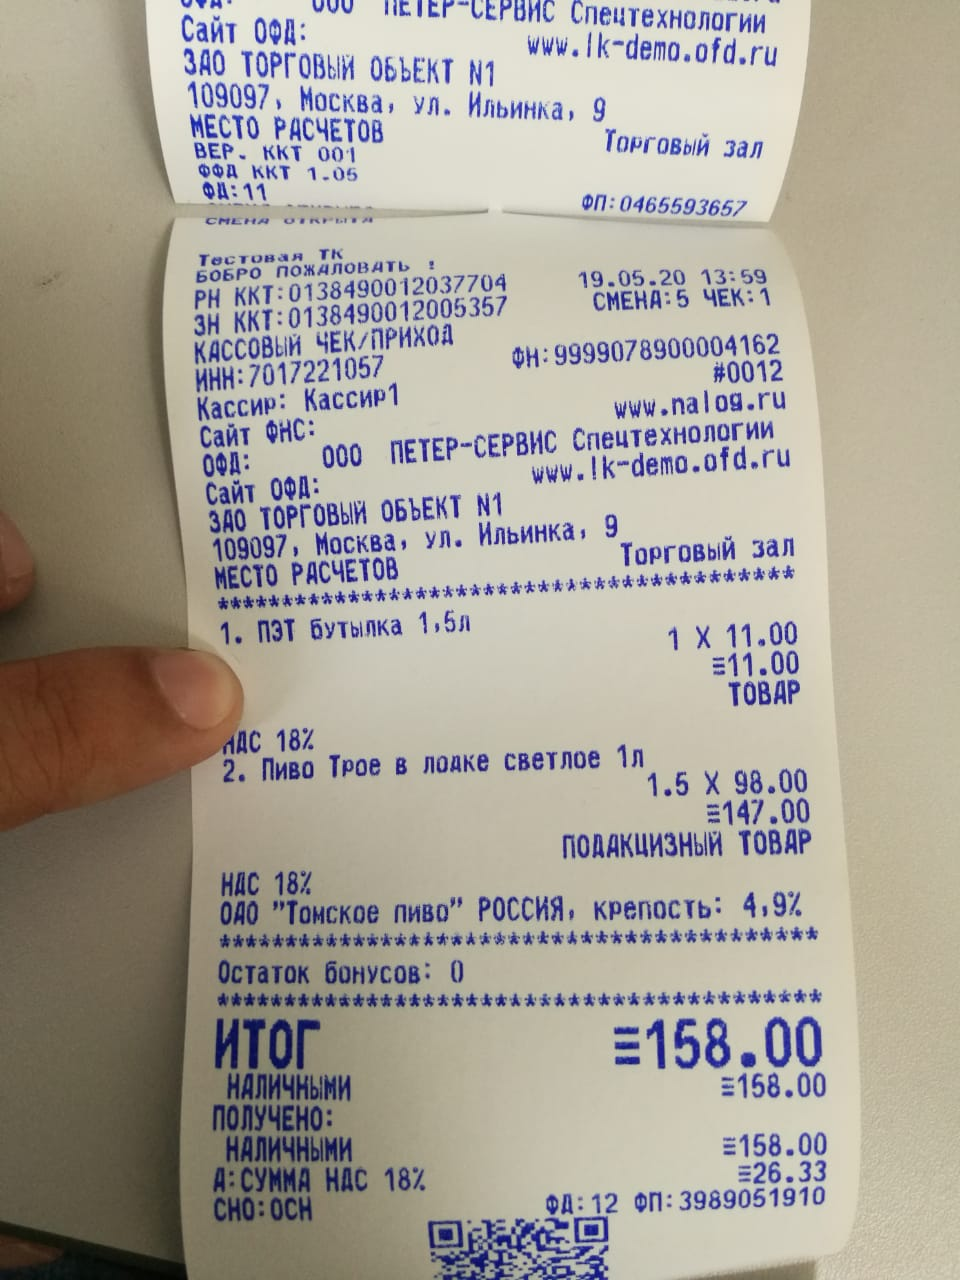
\includegraphics[width=125pt]{1.jpeg}} at (0pt,0pt)
\end{tikzpicture}
;\par
3. Поле <<СНО>> в чеке имеет значение <<ОСН>>;\par
4. Второй чек вида:
\begin{tikzpicture}
\pgftext{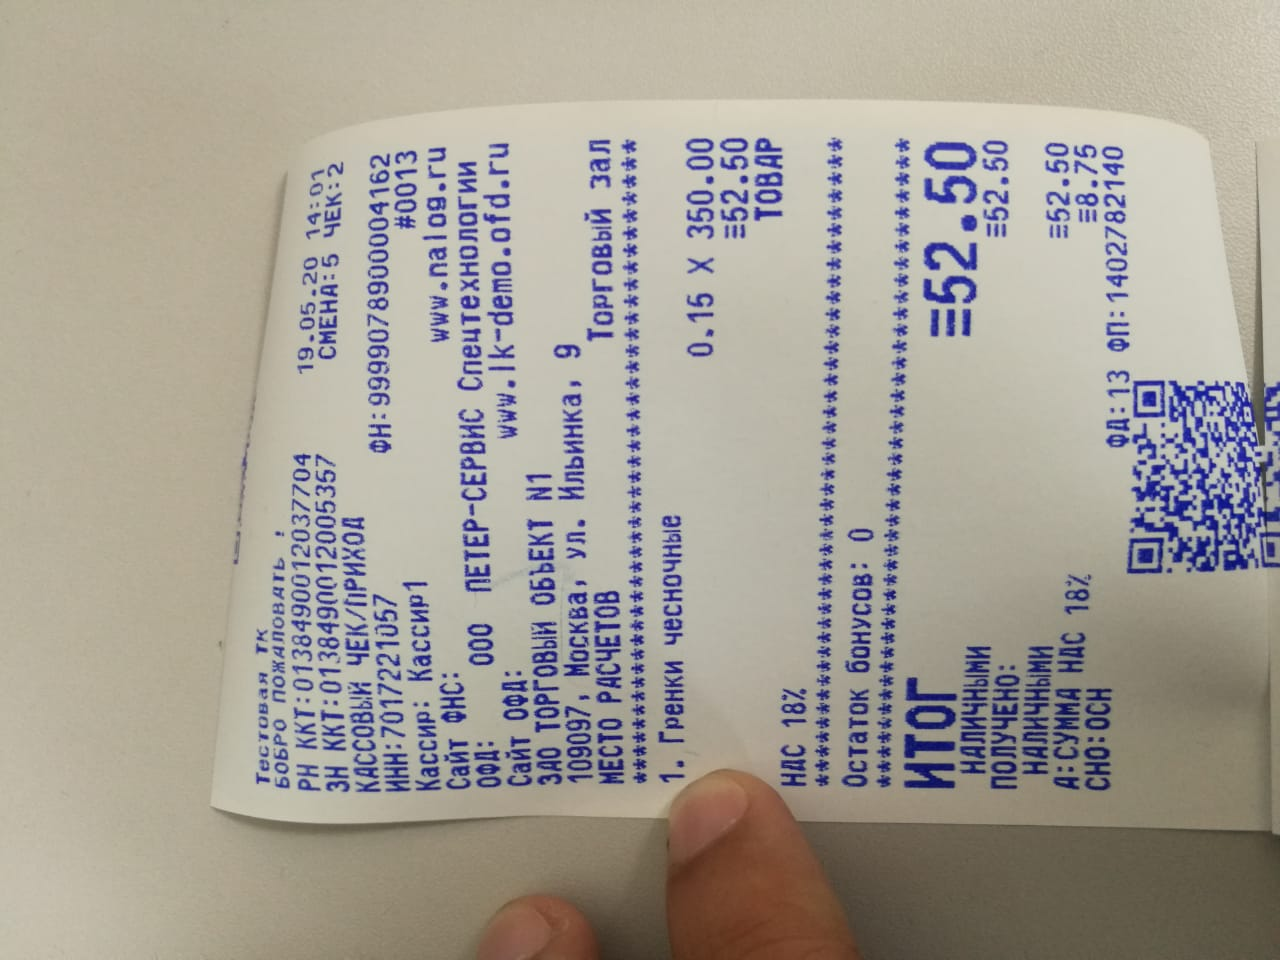
\includegraphics[width=125pt]{4.jpeg}} at (0pt,0pt)
\end{tikzpicture}
;\par
5. Поле <<СНО>> в чеке имеет значение <<УСН>>;\par
6. Табличная часть <<Товары>> в форме рабочего места кассира очистится;\par
&  \\
\hline
%****************************************************************************************************



\end{longtable}% Проверка чека с кулинарией и прочим товаром
\begin{longtable}{|p{0.02\linewidth}|p{0.3\linewidth}|p{0.3\linewidth}|p{0.3\linewidth}|}
    %  {|c|c|l|c|}
    \hline
    № & \textbf{Действие} & \textbf{Ожидаемый результат} & \textbf{Фактический результат} \\
    %****************************************************************************************************
    \hline
    \hline
    \endhead

   %****************************************************************************************************

   \multicolumn{4}{|c|}{\textbf{\textit{Проверка блокировки одновременной оплаты по безналичному расчету на разных кассах}}} \\
\hline
\hline
\Rownum &  Проверить, что включена константа «крюВключитьБлокировкуПараллельнойОплатыЭквайринг» включить если не включена & Включена константа «крюВключитьБлокировкуПараллельнойОплатыЭквайринг» &  \\
\hline
\Rownum &  Проверить, что включена константа «крюБлокировкаПараллельнойОплатыЭквайринг» включить если не включена & Включена константа «крюБлокировкаПараллельнойОплатыЭквайринг» &
\\
\hline
\Rownum & Запустить конфигурацию магазина выбрав пользователя <<Абрамовская Е. (кассир)>> & 1.Открылся общий интерфейс программы;\par
2. Отображаются разделы <<Главное>> и <<Продажи>>;\par
3. Открылась обработка <<Рабочее место кассира>>  &  \\
\hline
\Rownum	& Нажать кнопку \keys{Регистрация продаж} в меню РМК & 1. Форма меню РМК закрыта;\par
2. Открыта форма с информационным сообщением для кассиров;\par
3. Кнопка \keys{ОК} в нижней части формы недоступна &  \\
\hline
\Rownum	& Отметить чек бокс с надписью <<Мною прочитано и понято>> & 1. Чек бокс с надписью <<Мною прочитано и понято>> отмечен ;\par
2. Кнопка \keys{ОК} в нижней части формы доступна &   \\
\hline
\Rownum	& Нажать кнопку \keys{ОК} в нижней части формы & 1. Форма с информационным сообщением для кассиров закрыта.;\par
2. Открыта форма Рабочего места кассира  &  \\
\hline
\Rownum	& Нажать кнопку \keys{Поиск (F11)} в верхней части формы или горячую клавишу \keys{F11} & Открыта форма поиска и подбора товара в РМК &  \\
\hline
\Rownum	& Выбрать поиск по наименованию в выпадающем списке <<Поиск>> верхней части формы  & Выбран режим поиска по наименованию &  \\
\hline
\Rownum	& В поле поиска ввести <<Гренки чесночные>>  & В табличной части <<Товары>> осталась номенклатура, в наименовании которой содержится <<Гренки чесночные>> &  \\
\hline
\Rownum	& В табличной части <<Товары>> выбрать позицию с артикулом <<11432>>  & 1. Форма поиска закрылась;\par
2. В табличную часть <<Товары>> формы рабочего места кассира добавлена позиция с артикулом <<11432>> с количеством <<1>> и установленной ценой &  \\
\Rownum	& Установить количество позиции с артикулом <<11432>> равным <<0,150>>  & 1. Количество позиции с артикулом <<11432>> - <<Гренки чесночные>> изменилось на значение <<0,150>>&  \\
\hline

\Rownum	& Нажать кнопку \keys{Оплата (F8)} в верхней части формы или горячую клавишу \keys{F8}  &  Открыта форма оплаты &  \\
\hline
\Rownum	& Нажать кнопку \keys{Нал.(F6)} справа от поля ввода <<Всего к оплате (руб):>> или горячую клавишу \keys{F6}  & Появляется окно с сообщением <<"Осуществляется оплата по безналу на другой кассе, подождите...">> & !!!!!!!!!  \\
\hline

%****************************************************************************************************



\end{longtable}% Проверка блокировки одновременной оплаты по безналичному расчету на разных кассах
\begin{longtable}{|p{0.02\linewidth}|p{0.3\linewidth}|p{0.3\linewidth}|p{0.3\linewidth}|}
    %  {|c|c|l|c|}
    \hline
    № & \textbf{Действие} & \textbf{Ожидаемый результат} & \textbf{Фактический результат} \\
    %****************************************************************************************************
    \hline
    \hline
    \endhead

   %****************************************************************************************************

   \multicolumn{4}{|c|}{\textbf{\textit{Проверка записи в регистре сведений <<крю Этапы пробития чека ККМ>>}}} \\
\hline
\hline
\Rownum & Запустить конфигурацию магазина выбрав пользователя <<Абрамовская Е. (кассир)>> & 1.Открылся общий интерфейс программы;\par
2. Отображаются разделы <<Главное>> и <<Продажи>>;\par
3. Открылась обработка <<Рабочее место кассира>>  &  \\
\hline
\Rownum	& Нажать кнопку \keys{Регистрация продаж} в меню РМК & 1. Форма меню РМК закрыта;\par
2. Открыта форма с информационным сообщением для кассиров;\par
3. Кнопка \keys{ОК} в нижней части формы недоступна &  \\
\hline
\Rownum	& Отметить чек бокс с надписью <<Мною прочитано и понято>> & 1. Чек бокс с надписью <<Мною прочитано и понято>> отмечен ;\par
2. Кнопка \keys{ОК} в нижней части формы доступна &   \\
\hline
\Rownum	& Нажать кнопку \keys{ОК} в нижней части формы & 1. Форма с информационным сообщением для кассиров закрыта.;\par
2. Открыта форма Рабочего места кассира  &  \\
\hline
\Rownum	& Нажать кнопку \keys{Поиск (F11)} в верхней части формы или горячую клавишу \keys{F11} & Открыта форма поиска и подбора товара в РМК &  \\
\hline
\Rownum	& Выбрать поиск по наименованию в выпадающем списке <<Поиск>> верхней части формы  & Выбран режим поиска по наименованию &  \\
\hline
\Rownum	& В поле поиска ввести <<Трое в лодке светлое>>  & В табличной части <<Товары>> осталась номенклатура, в наименовании которой содержится <<Трое в лодке светлое>> &  \\
\hline
\Rownum	& В табличной части <<Товары>> выбрать позицию с артикулом <<11697>>  & 1. Форма поиска закрылась;\par
2. В табличную часть <<Товары>> формы рабочего места кассира добавлена позиция с артикулом <<11697>> с количеством <<1>> и установленной ценой &  \\
\hline
\Rownum	& Нажать кнопку \keys{Поиск (F11)} в верхней части формы или горячую клавишу \keys{F11} & Открыта форма поиска и подбора товара в РМК &  \\
\hline
\Rownum	& Выбрать поиск по наименованию в выпадающем списке <<Поиск>> верхней части формы  & Выбран режим поиска по наименованию &  \\
\hline
\Rownum	& В поле поиска ввести <<Пакет Крюгер Хаус маленький>>  & В табличной части <<Товары>> осталась номенклатура, в наименовании которой содержится <<Пакет Крюгер Хаус маленький>> &  \\
\hline
\Rownum	& В табличной части <<Товары>> выбрать позицию с артикулом <<10347>>  & 1. Форма поиска закрылась;\par
2. В табличную часть <<Товары>> формы рабочего места кассира добавлена позиция с артикулом <<10347>> с количеством <<1>> и установленной ценой &  \\
\hline
\Rownum	& Нажать \keys{Ctrl} + \keys{M}   & 1. В табличную часть <<Товары>> формы рабочего места кассира добавлена позиция с артикулом <<10340>> - <<ПЭТ бутылка 1,5л>>  &  \\
\hline
\Rownum	& Установить количество позиции с артикулом <<10340>> равным <<1>>  & 1. Количество позиции с артикулом <<11697>> - <<Пиво Трое в лодке светлое 1л>> изменилось на значение <<1.5>>&  \\
\hline
\Rownum	& Нажать кнопку \keys{Оплата (F8)} в верхней части формы или горячую клавишу \keys{F8}  &  Открыта форма оплаты &  \\
\hline
\Rownum	& Нажать кнопку \keys{ПК.(F7)} справа от поля ввода <<Всего к оплате (руб):>> или горячую клавишу    \keys{F7}  & В табличную часть <<Виды оплат>> добавлена строка со значениями полей: <<Вида оплаты>> - <<Оплата  картой>>; <<Сумма>> - рассчитанной суммой&  \\
\hline
\Rownum	& После предложения вставить карту, обратиться к сотруднику заказчика для осуществления оплаты картой  &  Оплата картой произведена&  \\
\hline
\Rownum	& Нажать кнопку \keys{Enter} в области цифровых кнопок или горячую клавишу \keys{Ctrl + Enter}  & 1. Форма оплаты закроется;\par
2. Табличная часть <<Товары>> в форме рабочего места кассира очистится&  \\
\hline
\Rownum & Закрыть рабочее место кассира нажав последовательно горячие клавиши \keys{F10} - \keys{F12}  & Открылось меню <<Рабочего места кассира>> &  \\
\hline
\Rownum & Нажать кнопку \keys{Завершение работы}   & Конфигурация закрылась
&  \\
\hline
\Rownum & Запустить конфигурацию магазина  & 1.Открылся общий интерфейс программы;\par
2. Отображаются все доступные разделы  &  \\
\hline
\Rownum & Перейти в раздел <<Продажи>>   & 1. Открылся отдел <<Продажи>>
&  \\
\hline
\Rownum	& Выбрать пункт  <<Чеки>> & Открылся форма списка документов <<Чек ККМ>> &  \\
&  \\
\hline
\Rownum & Выбрать последний созданный чек, открыть его  & Открылся форма  документа <<Чек ККМ>> &  \\
&  \\
\hline
\Rownum & Перейти на вкладку <<Комментарий>>  & 1. Открылась вкладка <<Комментарий>>;\par
2. Табличная часть под полем <<Комментарий>>, заполнена данными из регистра сведений <<крю Этапы пробития чека ККМ>> относящимися к текущему чеку ;\par
3. В поле <<Текст ЭЧ>> содержится полный текст чека эквайринга
;\par
4. В полях <<ЭЧ получен>>, <<ЭЧ распечатан>>, <<ФЧ распечатан>>, <<Безналичная оплата>> установлены зеленые <<галочки>>;\par
5. Поля <<Чек ККМ>>, <<Родитель чека ККМ>>, <<Предыдущий номер чека>>, <<Полученный номер чека>>, <<Касса ККМ>>, <<Сумма чека>> заполнены &  \\
&  \\
\hline
%****************************************************************************************************




\end{longtable}% Проверка записи в регистре сведений <<крю Этапы пробития чека ККМ>>
\begin{longtable}{|p{0.02\linewidth}|p{0.3\linewidth}|p{0.3\linewidth}|p{0.3\linewidth}|}
    %  {|c|c|l|c|}
    \hline
    № & \textbf{Действие} & \textbf{Ожидаемый результат} & \textbf{Фактический результат} \\
    %****************************************************************************************************
    \hline
    \hline
    \endhead

   %****************************************************************************************************

    \multicolumn{4}{|c|}{\textbf{\textit{В форме меню, если есть необработанные чеки блокируются все элементы кроме <<Регистрации продаж>> и сообщение разобраться с ошибками чеков}}} \\
\hline
\hline
\Rownum & Запустить конфигурацию магазина выбрав пользователя <<Абрамовская Е. (кассир)>> & 1.Открылся общий интерфейс программы;\par
2. Отображаются разделы <<Главное>> и <<Продажи>>;\par
3. Открылась обработка <<Рабочее место кассира>>  &  \\
\hline
\Rownum	& Нажать кнопку \keys{Регистрация продаж} в меню РМК & 1. Форма меню РМК закрыта;\par
2. Открыта форма с информационным сообщением для кассиров;\par
3. Кнопка \keys{ОК} в нижней части формы недоступна &  \\
\hline
\Rownum	& Отметить чек бокс с надписью <<Мною прочитано и понято>> & 1. Чек бокс с надписью <<Мною прочитано и понято>> отмечен ;\par
2. Кнопка \keys{ОК} в нижней части формы доступна &   \\
\hline
\Rownum	& Нажать кнопку \keys{ОК} в нижней части формы & 1. Форма с информационным сообщением для кассиров закрыта.;\par
2. Открыта форма Рабочего места кассира  &  \\
\hline
\Rownum	& Нажать кнопку \keys{Поиск (F11)} в верхней части формы или горячую клавишу \keys{F11} & Открыта форма поиска и подбора товара в РМК &  \\
\hline
\Rownum	& Выбрать поиск по наименованию в выпадающем списке <<Поиск>> верхней части формы  & Выбран режим поиска по наименованию &  \\
\hline
\Rownum	& В поле поиска ввести <<Трое в лодке светлое>>  & В табличной части <<Товары>> осталась номенклатура, в наименовании которой содержится <<Трое в лодке светлое>> &  \\
\hline
\Rownum	& В табличной части <<Товары>> выбрать позицию с артикулом <<11697>>  & 1. Форма поиска закрылась;\par
2. В табличную часть <<Товары>> формы рабочего места кассира добавлена позиция с артикулом <<11697>> с количеством <<1>> и установленной ценой &  \\
\hline
\Rownum	& Нажать кнопку \keys{Поиск (F11)} в верхней части формы или горячую клавишу \keys{F11} & Открыта форма поиска и подбора товара в РМК &  \\
\hline
\Rownum	& Выбрать поиск по наименованию в выпадающем списке <<Поиск>> верхней части формы  & Выбран режим поиска по наименованию &  \\
\hline
\Rownum	& В поле поиска ввести <<Пакет Крюгер Хаус маленький>>  & В табличной части <<Товары>> осталась номенклатура, в наименовании которой содержится <<Пакет Крюгер Хаус маленький>> &  \\
\hline
\Rownum	& В табличной части <<Товары>> выбрать позицию с артикулом <<10347>>  & 1. Форма поиска закрылась;\par
2. В табличную часть <<Товары>> формы рабочего места кассира добавлена позиция с артикулом <<10347>> с количеством <<1>> и установленной ценой &  \\
\hline
\Rownum	& Нажать \keys{Ctrl} + \keys{M}   & 1. В табличную часть <<Товары>> формы рабочего места кассира добавлена позиция с артикулом <<10340>> - <<ПЭТ бутылка 1,5л>>  &  \\
\hline
\Rownum	& Установить количество позиции с артикулом <<10340>> равным <<1>>  & 1. Количество позиции с артикулом <<11697>> - <<Пиво Трое в лодке светлое 1л>> изменилось на значение <<1.5>>&  \\
\hline
\Rownum	& Нажать кнопку \keys{Оплата (F8)} в верхней части формы или горячую клавишу \keys{F8}  &  Открыта форма оплаты &  \\
\hline
\Rownum	& Нажать кнопку \keys{Нал.(F6)} справа от поля ввода <<Всего к оплате (руб):>> или горячую клавишу \keys{F6}  & В табличную часть <<Виды оплат>> добавлена строка со значениями полей: <<Вида оплаты>> - <<Наличные>>; <<Сумма>> - рассчитанной суммой&  \\
\hline
\Rownum	& Нажать кнопку \keys{Enter} в области цифровых кнопок или горячую клавишу \keys{Ctrl + Enter} Передварительно связавшись с представителем заказчика, для отключения питания фискального регистратора в моментпробития чека, что бы инициировать ошибочную ситуацию  & 1. Форма оплаты закроется;\par
2. Табличная часть <<Товары>> в форме рабочего места кассира очистится&  \\
\hline

\Rownum & Закрыть рабочее место кассира нажав последовательно горячие клавиши \keys{F10} - \keys{F12}  &1.  Открылось меню <<Рабочего места кассира>>;\par
2. В меню доступны только кнопки: \keys{Регистрация продаж}, \keys{Закрыть}, \keys{Завершение работы}   &  \\
\hline
\Rownum & Нажать кнопку \keys{Завершение работы}   & Конфигурация закрылась
&  \\
\hline
\Rownum & Запустить конфигурацию магазина выбрав пользователя <<Абрамовская Е. (кассир)>> & 1.Открылся общий интерфейс программы;\par
2. Отображаются разделы <<Главное>> и <<Продажи>>;\par
3. Открылась обработка <<Рабочее место кассира>> ;\par
4. Открылась форма <<Ошибка непроведенных чеков>> с сообщением об ошибке <<Есть не обработанные чеки ККМ. Необходимо зайти «Регистрация продаж» -> Кнопка «Проверить Чеки ККМ» и проанализировать почему чек не пробит>> &  \\
\hline

\Rownum & Нажать кнопку \keys{Закрыть} на форме с описанием ошибки  & Форма с описанием ошибки закрылась
&  \\
\hline
\Rownum & Нажать кнопку \keys{Завершение работы}   & Конфигурация закрылась
&  \\
\hline
%****************************************************************************************************





\end{longtable}% В форме меню, если есть необработанные чеки блокируются все элементы кроме <<Регистрации продаж>> и сообщение разобраться с ошибками чеков
\begin{longtable}{|p{0.02\linewidth}|p{0.3\linewidth}|p{0.3\linewidth}|p{0.3\linewidth}|}
    %  {|c|c|l|c|}
    \hline
    № & \textbf{Действие} & \textbf{Ожидаемый результат} & \textbf{Фактический результат} \\
    %****************************************************************************************************
    \hline
    \hline
    \endhead

   %****************************************************************************************************

     \multicolumn{4}{|c|}{\textbf{\textit{При возникновении ошибок прежде чем пробивать новый чек, необходимо закончить работу со старым}}} \\
\hline
\hline
\Rownum & Запустить конфигурацию магазина выбрав пользователя <<Абрамовская Е. (кассир)>> & 1.Открылся общий интерфейс программы;\par
2. Отображаются разделы <<Главное>> и <<Продажи>>;\par
3. Открылась обработка <<Рабочее место кассира>> ;\par
4. Открылась форма <<Ошибка непроведенных чеков>> с сообщением об ошибке <<Есть не обработанные чеки ККМ. Необходимо зайти «Регистрация продаж» -> Кнопка «Проверить Чеки ККМ» и проанализировать почему чек не пробит>> &  \\
\hline
\Rownum & Нажать кнопку \keys{Закрыть} на форме с описанием ошибки  & Форма с описанием ошибки закрылась
&  \\
\hline
\Rownum	& Нажать кнопку \keys{Регистрация продаж} в меню РМК & 1. Форма меню РМК закрыта;\par
2. Открыта форма с информационным сообщением для кассиров;\par
3. Кнопка \keys{ОК} в нижней части формы недоступна &  \\
\hline
\Rownum	& Отметить чек бокс с надписью <<Мною прочитано и понято>> & 1. Чек бокс с надписью <<Мною прочитано и понято>> отмечен ;\par
2. Кнопка \keys{ОК} в нижней части формы доступна &   \\
\hline
\Rownum	& Нажать кнопку \keys{ОК} в нижней части формы & 1. Форма с информационным сообщением для кассиров закрыта.;\par
2. Открыта форма Рабочего места кассира  &  \\
\hline
\Rownum	& Нажать кнопку \keys{Поиск (F11)} в верхней части формы или горячую клавишу \keys{F11} & Открыта форма поиска и подбора товара в РМК &  \\
\hline
\Rownum	& Выбрать поиск по наименованию в выпадающем списке <<Поиск>> верхней части формы  & Выбран режим поиска по наименованию &  \\
\hline
\Rownum	& В поле поиска ввести <<Трое в лодке светлое>>  & В табличной части <<Товары>> осталась номенклатура, в наименовании которой содержится <<Трое в лодке светлое>> &  \\
\hline
\Rownum	& В табличной части <<Товары>> выбрать позицию с артикулом <<11697>>  & 1. Форма поиска закрылась;\par
2. Под табличной частью <<Товары>> появилось сообщение об ошибке содержащее номер чека, вид оплаты и сообщением <<Для дальнейшей работы на данной кассе требуется устранить указанную проблему!>>, ниже выводится еще одно сообщение <<Нажмите кнопку «Проверить Чеки ККМ»>>
&  \\
\hline
\Rownum	& Закрыть сообщение об ошибке & 1. Сообщение об ошибке закрылось;\par
2. Табличная часть <<Товары>> не содержит строк. &  \\
\hline

\Rownum & Закрыть рабочее место кассира нажав последовательно горячие клавиши \keys{F10} - \keys{F12}  &1.  Открылось меню <<Рабочего места кассира>>;\par
2. В меню доступны только кнопки: \keys{Регистрация продаж}, \keys{Закрыть}, \keys{Завершение работы}   &  \\
\hline
\Rownum & Нажать кнопку \keys{Завершение работы}   & Конфигурация закрылась
&  \\
\hline
%****************************************************************************************************


\end{longtable}% {При возникновении ошибок прежде чем пробивать новый чек, необходимо закончить работу со старым








%\input{rmk/}{ZapuskPriStarte}
%\end{longtable}%

%******************************************************
%               ЕГАИС
\newpage
\section{ЕГАИС}
\subsection{Объекты тестирования, описанные в разделе}

Тестирование рабочего места кассира нужно проводить на кассе и только при подключенном оборудовании ( фискальные регистратор, сканер штрихкодов, весы, табло покупателя)
\begin{longtable}{p{0.05\linewidth}p{0.4\linewidth}p{0.4\linewidth}}
    %  \toprule

   	\hline
   	1 & Вид объекта  & Документ \\
   	\hline
   	& Имя & ТТНВходящаяЕГАИС \\
   	\hline
   	& Синоним  & Товарно-транспортная накладная ЕГАИС (входящая) \\
   	\hline
%   	2 & Вид объекта  & Документ \\
%   	\hline
%   	& Имя & ТТНИсходящаяЕГАИС \\
%   	\hline
%   	& Синоним  & Товарно-транспортная накладная ЕГАИС (исходящая) \\
%   	\hline
     2 & Вид объекта  & Документ \\
    \hline
    & Имя & АктПостановкиНаБалансЕГАИС \\
    \hline
    & Синоним  & Акт постановки на баланс ЕГАИС \\
    \hline
    3 & Вид объекта  & Документ \\
    \hline
    & Имя & АктСписанияЕГАИС \\
    \hline
    & Синоним  & Акт списания ЕГАИС \\
    \hline
    4 & Вид объекта  & Документ \\
    \hline
    & Имя & ПередачаВРегистр2ЕГАИС \\
    \hline
    & Синоним  & Передача в регистр №2 ЕГАИС \\
    \hline
    5 & Вид объекта  & Документ \\
    \hline
    & Имя & ВозвратИзРегистра2ЕГАИС \\
    \hline
    & Синоним  & Возврат из регистра №2 ЕГАИС \\
    \hline
     6 & Вид объекта & Документ \\
    \hline
    %     \hline
    %    \endhead
    & Имя & Проверка алгоритмов \\
    \hline
    & Синоним  & Проверка алгоритмов \\
    \hline
    \bottomrule %%% верхняя линейка
\end{longtable}
% ЕГАИС
\newpage
\subsection{Формирование документа Товарно-транспортная накладная ЕГАИС (входящая)}

\begin{warning}
    \textbf{Внимание!!!! Тестирование работы ЕГАИС производится в сотрудничестве со специалистом заказчика. (если не будет предоставлен дополнительный доступ к тестовым серверам) \\
        Упоминание в тексте заказчика означает необходимость выполнения действий с его стороны.}
\end{warning}



\renewcommand{\arraystretch}{1.8} %% расстояние между строками таблицы
%\begin{landscape}
\begin{longtable}{|p{0.02\linewidth}|p{0.3\linewidth}|p{0.3\linewidth}|p{0.3\linewidth}|}
    %  {|c|c|l|c|}
    \hline
    № & \textbf{Действие} & \textbf{Ожидаемый результат} & \textbf{Фактический результат} \\
    %****************************************************************************************************
   \hline
   \hline
   \Rownum & Запустить конфигурацию магазина  & 1.Открылся общий интерфейс программы;\par
   2. Отображаются все доступные разделы  &  \\
   \hline
   \Rownum & Перейти в раздел <<Закупки>>   & 1. Открылся отдел <<Закупки>>
   &  \\

   \hline
   \Rownum	& Выбрать пункт <<Входящие ТТН>>  & Открылся журнал документов <<Входящие товарно-транспортные накладные ЕГАИС>>   &  \\
    \Rownum	& Нажать кнопку \keys{Выполнить обмен} в шапке жернала & 1. Выполнился обмен с транспортным модулем ЕГАИС;\par
    2. Произошла загрузка документов <<Товарно-транспортная накладная ЕГАИС (входящая)>>;\par
    3. Статус у загруженных документов <<Принят из ЕГАИС>> ;\par
    4. Значение в колонке <<Дальнейшее действие>> <<Выполните проверку>>  &  \\
    \hline
    \Rownum	& Открыть первый из  поступивших документов <<Товарно-транспортная накладная ЕГАИС (входящая)>>  & 1. Открыта форма документа <<Товарно-транспортная накладная ЕГАИС (входящая)>>;\par
    2. В шапке документы надписи имеют следующие значения: <<Статус: Принят из ЕГАИС>>, <<Выполните проверку или откажитесь от накладной>> &   \\
    \hline
    \Rownum	& Переключится на вкладку <<Товары>>  & Открыта вкладка <<Товары>> &  \\
    \hline
    \Rownum	& Кликнуть на надпись <<Проверить поступившую алкогольную продукцию>> & Открыта форма документа <<Проверка поступившей алкогольной продукции>> &  \\
    \hline
    \Rownum	& Кликнуть на надпись <<Проверить поступившую алкогольную продукцию>> & Открыта форма  <<Проверка поступившей алкогольной продукции>> &  \\
    \hline
    \Rownum	& Нажать кнопку \keys{Заполнить фактическое количество}  & Колонка <<Факт>> в табличной части формы заполнена количеством равным количеству в колонке <<По документу>>&  \\
    \hline
    \Rownum	& Нажать кнопку \keys{Проверка завершена}  & 1. Форма  <<Проверка поступившей алкогольной продукции>> закрыта;\par
    2. Текст надписи <<Проверить поступившую алкогольную продукцию>> изменился на <<Результаты проверки алкогольной продукции>>;\par
    3. В шапке документа текст надписи  <<Выполните проверку или откажитесь от накладной>> изменился на <<Подтвердите получение или откажитесь от накладной>>   &  \\
    \hline
    \Rownum	& Переключится на вкладку <<Основное>>  & Открыта вкладка <<Основное>> &  \\
    \hline
    \Rownum	& Кликнуть на надпись <<Оформить поступление>> справ от поля ввода <<Документ поступления>> & 1. Открыта форма нового документа <<Поступление товаров>>;\par
    2. Шапка и табличная часть заполнена данными из текущего документа <<Товарно-транспортная накладная ЕГАИС (входящая)>>;\par
    3. Количество в табличной части корректно пересчитано из даллов в литры &  \\
    \hline
    \Rownum	& Нажать кнопку \keys{Провести и закрыть} & 1. Форма  документа <<Поступление товаров>> закрыта;\par
    2. Открыта форма текущего документа <<Товарно-транспортная накладная ЕГАИС (входящая)>> &  \\
    \hline

    \Rownum	& Кликнуть на надпись <<Подтвердите получение>> & Текст надписей <<Статус: Принят из ЕГАИС>> и <<Подтвердите получение или откажитесь от накладной>> изменился на <<Статус: К подтверждению (передан в УТМ)>>  &  \\
    \hline

    \Rownum	& Нажать кнопку \keys{Провести и закрыть} & Форма  документа  <<Товарно-транспортная накладная ЕГАИС (входящая)>> закрыта&  \\
    \hline
    \Rownum	& Нажать кнопку \keys{Выполнить обмен} & 1. Статус  документа  <<Товарно-транспортная накладная ЕГАИС (входящая)>> сменился на <<К подтверждению (передан в УТМ)>>, а значение в колонке <<Дальнейшее действие>> на <<Ожидайте получения квитанции получен ЕГАИС>>&  \\
    \hline
    \Rownum	& Попросите специалиста заказчика подтвердить накладную & &  \\
    \hline
    \Rownum	& Нажать кнопку \keys{Выполнить обмен} & 1. Статус  документа  <<Товарно-транспортная накладная ЕГАИС (входящая)>> сменился на <<Подтвержден>>, а значение в колонке <<Дальнейшее действие>> на <<Не требуется>>&  \\
    \hline


    %****************************************************************************************************


\end{longtable}% Табак
%\newpage
%\subsection{Формирование документа Товарно-транспортная накладная ЕГАИС (исходящая)}

\renewcommand{\arraystretch}{1.8} %% расстояние между строками таблицы
%\begin{landscape}
\begin{longtable}{|p{0.02\linewidth}|p{0.3\linewidth}|p{0.3\linewidth}|p{0.3\linewidth}|}
    %  {|c|c|l|c|}
    \hline
    № & \textbf{Действие} & \textbf{Ожидаемый результат} & \textbf{Фактический результат} \\
    %****************************************************************************************************
       \hline
    \hline
    \endhead
    \multicolumn{4}{|c|}{\textbf{\textit{******}}} \\
    \hline
    \hline

    %****************************************************************************************************


\end{longtable}% Сервис
\subsection{Формирование документа Акт постановки на баланс ЕГАИС}

\begin{longtable}{|p{0.02\linewidth}|p{0.3\linewidth}|p{0.3\linewidth}|p{0.3\linewidth}|}
    %  {|c|c|l|c|}
    \hline
    № & \textbf{Действие} & \textbf{Ожидаемый результат} & \textbf{Фактический результат} \\
    %****************************************************************************************************
    \hline
    \hline
    \endhead
    \multicolumn{4}{|c|}{\textbf{\textit{Проверка на наличие и функцию кнопки Акт постановки на баланс ЕГАИС}}} \\
    \hline

    \hline
    \Rownum &  Перейти в раздел Склад, выбрать <<Акты постановки на баланс>>.  & 1. Открылся список документов  <<Акт постановки на баланс ЕГАИС>>;\par
    2. Отображаются все документы &  \\
    \hline
    \Rownum & Открыть существующий документ  & 1. Открылась форма существующего документа
    &  \\

    \hline
    \Rownum	& Убедится в наличии кнопки  \keys{Акт постановки на баланс ЕГАИС}   & Кнопка  \keys{Акт постановки на баланс ЕГАИС} присутствует  &  \\
    \hline
    \Rownum	& Нажать на кнопку  \keys{Акт постановки на баланс ЕГАИС}   & Сформирована печатная форма <<Акт постановки на баланс ЕГАИС>>  &  \\
    \hline
    %****************************************************************************************************



    %****************************************************************************************************

    \multicolumn{4}{|c|}{\textbf{\textit{Движение по регистру <<Остатки алкогольной продукции в торговом зале ЕГАИС>>}}} \\
    \hline

    \hline
    \Rownum &  Перейти в раздел Склад, выбрать <<Акты постановки на баланс>>.  & 1. Открылся список документов  <<Акт постановки на баланс ЕГАИС>>;\par
    2. Отображаются все документы &  \\
    \hline
    \Rownum & Открыть существующий документ  & 1. Открылась форма существующего документа
    &  \\
    \hline
    \Rownum	& Нажать кнопку \keys{Провести} &  Документ проводится без ошибок &  \\
    \hline
    \Rownum	& Выбрать команду <<Движения документа>> & Откроется отчет по движениям документа &  \\
    \hline
    \Rownum	& Найти в отчете движения по регистру <<Остатки алкогольной продукции в торговом зале ЕГАИС>> & Движения документа по регистру сведений <<Остатки алкогольной продукции в торговом зале ЕГАИС>> присутствуют. Измерения <<Период>>, <<Организация ЕГАИС>>,<<Склад>>, <<Номенклатура>>, <<Алкогольная продукция>>, <<Справка Б>>, <<Документ приход>> заполнены. Значение ресурса <<Количество упаковок>> заполнено  &  \\
    \hline
    %****************************************************************************************************
\end{longtable}
% Акт постановки на баланс ЕГАИС
\newpage
\subsection{Формирование документа Акт списания ЕГАИС}

\renewcommand{\arraystretch}{1.8} %% расстояние между строками таблицы
%\begin{landscape}
\begin{longtable}{|p{0.02\linewidth}|p{0.3\linewidth}|p{0.3\linewidth}|p{0.3\linewidth}|}
    \hline
    № & \textbf{Действие} & \textbf{Ожидаемый результат} & \textbf{Фактический результат} \\
    %****************************************************************************************************
    \hline
    \hline
    \endhead
    \multicolumn{4}{|c|}{\textbf{\textit{Проверка на наличие и функцию кнопки <<Перезаполнить на основании ОРП>>}}} \\
    \hline

    \hline
    \Rownum &  Перейти в раздел Склад, выбрать <<Акты списания>>.  & 1. Открылся список документов  <<Акты списания ЕГАИС>>;\par
    2. Отображаются все документы &  \\
    \hline
    \Rownum & Открыть существующий документ  & 1. Открылась форма существующего документа
    &  \\

    \hline
    \Rownum	& Убедится в наличии кнопки  \keys{Перезаполнить на основании ОРП}   & Кнопка  \keys{Перезаполнить на основании ОРП} присутствует  &  \\
    \hline
    \Rownum	& Убедиться, что документ создан на основании документа <<Отчет о розничных продажах>> (проверив реквизит <<Основание>>), если это не так, выбрать другой документ & Выбран документ созданный на основании документа <<Отчет о розничных продажах>>   &  \\
    \hline
    \Rownum	& Открыть документ основание  & Открыт документ <<Отчет о розничных продажах>>  &  \\
    \hline

    \Rownum	& Удалить из табличной части <<Товары>> строки с алкогольной продукцией & Из табличной части товары документа <<Отчет о розничных продажах>> удалены строки с алкогольной продукцией &  \\
    \hline

    \Rownum	& Нажать кнопку \keys{Провести и закрыть}  & Документ <<Отчет о розничных продажах>> проведен и закрыт  &  \\

    \hline
    \Rownum	& Нажать на кнопку  \keys{Перезаполнить на основании ОРП} в документе <<Акт списания ЕГАИС>>.  & Табличная часть <<Товары>> документа  <<Акт списания ЕГАИС>>, очищена  &  \\
    \hline
%****************************************************************************************************

  \multicolumn{4}{|c|}{\textbf{\textit{Проверка на наличие и функцию кнопки<<Акт списания ЕГАИС>> }}} \\
  \hline

  \hline
  \Rownum &  Перейти в раздел Склад, выбрать <<Акты списания>>.  & 1. Открылся список документов  <<Акт списания ЕГАИС>>;\par
  2. Отображаются все документы &  \\
  \hline
  \Rownum & Открыть существующий документ  & 1. Открылась форма существующего документа
  &  \\

  \hline
  \Rownum	& Убедится в наличии кнопки  \keys{Акт списания ЕГАИС}   & Кнопка  \keys{Акт списания ЕГАИС} присутствует  &  \\
  \hline
  \Rownum	& Нажать на кнопку  \keys{Акт списания ЕГАИС}   & Сформирована печатная форма <<Акт списания ЕГАИС>>  &  \\
  \hline
  %****************************************************************************************************


%****************************************************************************************************

    \multicolumn{4}{|c|}{\textbf{\textit{Движение по регистру <<Остатки алкогольной продукции в торговом зале ЕГАИС>>}}} \\
    \hline
    \hline
    \Rownum &  Перейти в раздел Склад, выбрать <<Акты списания>>.  & 1. Открылся список документов  <<Акт списания ЕГАИС>>;\par
    2. Отображаются все документы &  \\
    \hline
    \Rownum & Открыть существующий документ  & 1. Открылась форма существующего документа
    &  \\
    \hline
    \Rownum	& Нажать кнопку \keys{Провести} &  Документ проводится без ошибок &  \\
    \hline
    \Rownum	& Выбрать команду <<Движения документа>> & Откроется отчет по движениям документа &  \\
    \hline
    \Rownum	& Найти в отчете движения по регистру <<Остатки алкогольной продукции в торговом зале ЕГАИС>> & Движения документа по регистру сведений <<Остатки алкогольной продукции в торговом зале ЕГАИС>> присутствуют. Измерения <<Период>>, <<Организация ЕГАИС>>,<<Склад>>, <<Номенклатура>>, <<Алкогольная продукция>>, <<Справка Б>>, <<Документ приход>> заполнены. Значение ресурса <<Количество упаковок>> заполнено  &  \\
    \hline
%****************************************************************************************************


    %  {|c|c|l|c|}

%****************************************************************************************************
\hline

\multicolumn{4}{|c|}{\textbf{\textit{Акт списания создается на начало дня при закрытии смены}}} \\
\hline
\hline
 \hline
\Rownum	& \cool\ &   &  \\
\hline
%****************************************************************************************************

    %  {|c|c|l|c|}

%****************************************************************************************************
\hline

\multicolumn{4}{|c|}{\textbf{\textit{При установленной константе "крюОтправлятьАктыЕГАИСПриЗакрытииСмены"Акты списания отправляются при закрытии кассовой смены}}} \\
\hline
 \hline
\Rownum	& \cool\ &   &  \\
\hline

%****************************************************************************************************



\end{longtable}% Акт списания ЕГАИС
\newpage
\subsection{Формирование документа Передача в регистр №2 ЕГАИС}

\renewcommand{\arraystretch}{1.8} %% расстояние между строками таблицы
%\begin{landscape}
\begin{longtable}{|p{0.02\linewidth}|p{0.3\linewidth}|p{0.3\linewidth}|p{0.3\linewidth}|}


%****************************************************************************************************
 \hline
\multicolumn{4}{|c|}{\textbf{\textit{Движение по регистру <<Остатки алкогольной продукции в торговом зале ЕГАИС>>}}} \\
\hline

\hline
\Rownum &  Перейти в раздел Склад, выбрать <<Передачи в регистр №2>>.  & 1. Открылся список документов  <<Передачи в регистр №2>>;\par
2. Отображаются все документы &  \\
\hline
\Rownum & Открыть существующий документ  & 1. Открылась форма существующего документа
&  \\
\hline
\Rownum	& Нажать кнопку \keys{Провести} &  Документ проводится без ошибок &  \\
\hline
\Rownum	& Выбрать команду <<Движения документа>> & Откроется отчет по движениям документа &  \\
\hline
\Rownum	& Найти в отчете движения по регистру <<Остатки алкогольной продукции в торговом зале ЕГАИС>> & Движения документа по регистру сведений <<Остатки алкогольной продукции в торговом зале ЕГАИС>> присутствуют. Измерения <<Период>>, <<Организация ЕГАИС>>,<<Склад>>, <<Номенклатура>>, <<Алкогольная продукция>>, <<Справка Б>>, <<Документ приход>> заполнены. Значение ресурса <<Количество упаковок>> заполнено  &  \\
\hline
%****************************************************************************************************
\end{longtable}% Передача в регистр 2 ЕГАИС
\newpage
\subsection{Формирование документа Возврат из регистра №2 ЕГАИС}

\renewcommand{\arraystretch}{1.8} %% расстояние между строками таблицы
%\begin{landscape}
\begin{longtable}{|p{0.02\linewidth}|p{0.3\linewidth}|p{0.3\linewidth}|p{0.3\linewidth}|}


    %****************************************************************************************************
     \hline
    \multicolumn{4}{|c|}{\textbf{\textit{Движение по регистру <<Остатки алкогольной продукции в торговом зале ЕГАИС>>}}} \\
    \hline

    \hline
    \Rownum &  Перейти в раздел Склад, выбрать <<Возвраты из регистра №2>>.  & 1. Открылся список документов  <<Возвраты из регистра №2>>;\par
    2. Отображаются все документы &  \\
    \hline
    \Rownum & Открыть существующий документ имеющий статус <<Проведен в ЕГАИС>>  & 1. Открылась форма существующего документа;\par
    2. Статус документа имеет значение <<Проведен в ЕГАИС>>
    &  \\
    \hline
    \Rownum	& Нажать кнопку \keys{Провести} &  Документ проводится без ошибок &  \\
    \hline
    \Rownum	& Выбрать команду <<Движения документа>> & Откроется отчет по движениям документа &  \\
    \hline
    \Rownum	& Найти в отчете движения по регистру <<Остатки алкогольной продукции в торговом зале ЕГАИС>> & Движения документа по регистру сведений <<Остатки алкогольной продукции в торговом зале ЕГАИС>> присутствуют. Измерения <<Период>>, <<Организация ЕГАИС>>,<<Склад>>, <<Номенклатура>>, <<Алкогольная продукция>>, <<Справка Б>>, <<Документ приход>> заполнены. Значение ресурса <<Количество упаковок>> заполнено  &  \\
    \hline
    %****************************************************************************************************
\end{longtable}% Возврат из регистар 2 ЕГАИС
\newpage
\newpage
\subsection{Проверка алгоритмов ЕГАИС}

\renewcommand{\arraystretch}{1.8} %% расстояние между строками таблицы
%\begin{landscape}
\begin{longtable}{|p{0.02\linewidth}|p{0.3\linewidth}|p{0.3\linewidth}|p{0.3\linewidth}|}
    %  {|c|c|l|c|}
    \hline
    № & \textbf{Действие} & \textbf{Ожидаемый результат} & \textbf{Фактический результат} \\
    %****************************************************************************************************
    \hline
    \hline
    \endhead
    \multicolumn{4}{|c|}{\textbf{\textit{******}}} \\
    \hline
    \hline

    %****************************************************************************************************


\end{longtable}

\newpage
\section{Справочники}
\subsection{Объекты тестирования, описанные в разделе}

\begin{longtable}{p{0.05\linewidth}p{0.4\linewidth}p{0.4\linewidth}}
    %  \toprule
    \hline
    1 & Вид объекта & Справочник \\
    \hline
     & Имя & Номенклатура \\
    \hline
    & Синоним  & Номенклатура \\
    \hline


    \bottomrule %%% верхняя линейка
\end{longtable}% Дополнительные описания

\newpage
\section{Сервис}

\subsection{Объекты тестирования, описанные в разделе}

\begin{tabular}{p{0.05\linewidth}p{0.4\linewidth}p{0.4\linewidth}}
    \toprule
    %	\hline
    1 & Вид объекта & Документ \\
    \hline
    & Имя & крюКонтрольМинимальногоОстаткаКлючевыхПозиций \\
    \hline
    & Синоним  & Контроль минимального остатка ключевых позиций \\
    \hline
    2 & Вид объекта  & Обработка \\
    \hline
    & Имя & ПечатьЭтикетокИЦенников \\
    \hline
    & Синоним  & Печать этикеток и ценников \\
    \hline
    3 & Вид объекта  & Обработка \\
    \hline

    %	\hline
    \bottomrule %%% верхняя линейка
\end{tabular}



 % Описание прочих изменений
\newpage

\newpage
\subsection{Контроль минимального остатка ключевого товара}

\renewcommand{\arraystretch}{1.8} %% расстояние между строками таблицы
\begin{longtable}{|p{0.02\linewidth}|p{0.3\linewidth}|p{0.3\linewidth}|p{0.3\linewidth}|}
    %  {|c|c|l|c|}
    \hline
    № & \textbf{Действие} & \textbf{Ожидаемый результат} & \textbf{Фактический результат} \\
    %****************************************************************************************************
    \hline
    \hline
    \endhead
    \multicolumn{4}{|c|}{\textbf{\textit{Проверка работы алгоритма проверки остатков товара}}} \\
    \hline
    \Rownum & Проверить наличие регистра <<крюМинимальныеОстаткиКлючевойТовар>>  & Регистр <<крюМинимальныеОстаткиКлючевойТовар>> существует &  \\
    \hline
    \Rownum & Открыть регистр <<крюМинимальныеОстаткиКлючевойТовар>>  & Открылась форма списка регистра <<крюМинимальныеОстаткиКлючевойТовар>> \par
    &  \\
    \hline
      \Rownum & Убедиться в наличи записей в регистре  & В регистре <<крюМинимальныеОстаткиКлючевойТовар>> присутствуют записи.\par
    &  \\
    \hline
    %****************************************************************************************************





    %****************************************************************************************************
\end{longtable}
 % Описание прочих изменений
\newpage

\newpage
\section{Недописанное и шаблоны}
\subsection{Добавить в РМК (управляемый режим)}
\renewcommand{\arraystretch}{1.8} %% расстояние между строками таблицы
%\begin{landscape}
\begin{longtable}{|p{0.02\linewidth}|p{0.3\linewidth}|p{0.3\linewidth}|p{0.3\linewidth}|}
 \multicolumn{4}{|c|}{\textbf{\textit{Проверка блокировки возврата покупателю при сложных чеках и оплате по безналичному расчету}}} \\
   \hline
   \hline
   \Rownum & Запустить конфигурацию магазина выбрав пользователя <<Абрамовская Е. (кассир)>> & 1.Открылся общий интерфейс программы;\par
   2. Отображаются разделы <<Главное>> и <<Продажи>>;\par
   3. Открылась обработка <<Рабочее место кассира>>  &  \\
   \hline
   \Rownum	& Нажать кнопку \keys{Регистрация продаж} в меню РМК & 1. Форма меню РМК закрыта;\par
   2. Открыта форма с информационным сообщением для кассиров;\par
   3. Кнопка \keys{ОК} в нижней части формы недоступна &  \\
   \hline
   \Rownum	& Отметить чек бокс с надписью <<Мною прочитано и понято>> & 1. Чек бокс с надписью <<Мною прочитано и понято>> отмечен ;\par
   2. Кнопка \keys{ОК} в нижней части формы доступна &   \\
   \hline
   \Rownum	& Нажать кнопку \keys{ОК} в нижней части формы & 1. Форма с информационным сообщением для кассиров закрыта.;\par
   2. Открыта форма Рабочего места кассира  &  \\
   \hline
   \Rownum	& Нажать кнопку \keys{Поиск (F11)} в верхней части формы или горячую клавишу \keys{F11} & Открыта форма поиска и подбора товара в РМК &  \\
   \hline
   \Rownum	& Выбрать поиск по наименованию в выпадающем списке <<Поиск>> верхней части формы  & Выбран режим поиска по наименованию &  \\
   \hline
   \Rownum	& В поле поиска ввести <<Гренки чесночные>>  & В табличной части <<Товары>> осталась номенклатура, в наименовании которой содержится <<Гренки чесночные>> &  \\
   \hline
   \Rownum	& В табличной части <<Товары>> выбрать позицию с артикулом <<11432>>  & 1. Форма поиска закрылась;\par
   2. В табличную часть <<Товары>> формы рабочего места кассира добавлена позиция с артикулом <<11432>> с количеством <<1>> и установленной ценой &  \\
   \Rownum	& Установить количество позиции с артикулом <<11432>> равным <<0,150>>  & 1. Количество позиции с артикулом <<11432>> - <<Гренки чесночные>> изменилось на значение <<0,150>>&  \\
   \hline
   \Rownum	& Нажать кнопку \keys{Поиск (F11)} в верхней части формы или горячую клавишу \keys{F11} & Открыта форма поиска и подбора товара в РМК &  \\
   \hline
   \Rownum	& Выбрать поиск по наименованию в выпадающем списке <<Поиск>> верхней части формы  & Выбран режим поиска по наименованию &  \\
   \hline
   \Rownum	& В поле поиска ввести <<Трое в лодке светлое>>  & В табличной части <<Товары>> осталась номенклатура, в наименовании которой содержится <<Трое в лодке светлое>> &  \\
   \hline
   \Rownum	& В табличной части <<Товары>> выбрать позицию с артикулом <<11697>>  & 1. Форма поиска закрылась;\par
   2. В табличную часть <<Товары>> формы рабочего места кассира добавлена позиция с артикулом <<11697>> с количеством <<1>> и установленной ценой &  \\
   \hline
   \Rownum	& Нажать \keys{Ctrl} + \keys{M}   & 1. В табличную часть <<Товары>> формы рабочего места кассира добавлена позиция с артикулом <<10340>> - <<ПЭТ бутылка 1,5л>>  &  \\
   \hline
   \Rownum	& Установить количество позиции с артикулом <<10340>> равным <<1>>  & 1. Количество позиции с артикулом <<11697>> - <<Пиво Трое в лодке светлое 1л>> изменилось на значение <<1.5>>&  \\
   \hline
   \Rownum	& Нажать кнопку \keys{Оплата (F8)} в верхней части формы или горячую клавишу \keys{F8}  &  Открыта форма оплаты &  \\
   \hline
   \Rownum	& Нажать кнопку \keys{Нал.(F6)} справа от поля ввода <<Всего к оплате (руб):>> или горячую клавишу \keys{F6}  & В табличную часть <<Виды оплат>> добавлена строка со значениями полей: <<Вида оплаты>> - <<Наличные>>; <<Сумма>> - рассчитанной суммой&  \\
   \hline
   \Rownum	& Нажать кнопку \keys{Enter} в области цифровых кнопок или горячую клавишу \keys{Ctrl + Enter}  & 1. Форма оплаты закроется;\par
   2. На фискальном регистраторе будет напечатано два чека;\par
   3. Табличная часть <<Товары>> в форме рабочего места кассира очистится;\par
   &  \\
   \if 0
   Дописать возврат, вызов формы выбора чека и получения ошибки при двойном чеке и безнале
   \fi
   \hline
   %****************************************************************************************************


    \multicolumn{4}{|c|}{\textbf{\textit{В форме меню, если есть необработанные чеки блокируются все элементы кроме <<Регистрации продаж>> и сообщение разобраться с ошибками чеков}}} \\
   \hline
   \hline
   \Rownum & Запустить конфигурацию магазина выбрав пользователя <<Абрамовская Е. (кассир)>> & 1.Открылся общий интерфейс программы;\par
   2. Отображаются разделы <<Главное>> и <<Продажи>>;\par
   3. Открылась обработка <<Рабочее место кассира>>  &  \\

   \hline
   %****************************************************************************************************

     \multicolumn{4}{|c|}{\textbf{\textit{Анализ чека на наличие в нем сообщения об ошибке}}} \\
   \hline
   \hline
   \Rownum & Запустить конфигурацию магазина выбрав пользователя <<Абрамовская Е. (кассир)>> & 1.Открылся общий интерфейс программы;\par
   2. Отображаются разделы <<Главное>> и <<Продажи>>;\par
   3. Открылась обработка <<Рабочее место кассира>>  &  \\

   \hline
   %****************************************************************************************************


   \multicolumn{4}{|c|}{\textbf{\textit{Алгоритм фиксации времени прохождения этапов набора, проведения и пробития чека}}} \\
   \hline
   \hline
   \Rownum & Запустить конфигурацию магазина выбрав пользователя <<Абрамовская Е. (кассир)>> & 1.Открылся общий интерфейс программы;\par
   2. Отображаются разделы <<Главное>> и <<Продажи>>;\par
   3. Открылась обработка <<Рабочее место кассира>>  &  \\

   \hline
   %****************************************************************************************************

    \multicolumn{4}{|c|}{\textbf{\textit{При возникновении ошибок прежде чем пробивать новый чек, необходимо закончить работу со старым}}} \\
   \hline
   \hline
   \Rownum & Запустить конфигурацию магазина выбрав пользователя <<Абрамовская Е. (кассир)>> & 1.Открылся общий интерфейс программы;\par
   2. Отображаются разделы <<Главное>> и <<Продажи>>;\par
   3. Открылась обработка <<Рабочее место кассира>>  &  \\

   \hline
   %****************************************************************************************************


     \multicolumn{4}{|c|}{\textbf{\textit{Изменена основная форма РМК, уменьшен размер}}} \\
   \hline
   \hline
   \Rownum & Запустить конфигурацию магазина выбрав пользователя <<Абрамовская Е. (кассир)>> & 1.Открылся общий интерфейс программы;\par
   2. Отображаются разделы <<Главное>> и <<Продажи>>;\par
   3. Открылась обработка <<Рабочее место кассира>>  &  \\

   \hline
   %****************************************************************************************************
\end{longtable}
% РМК



%\listoffigures
%\newpage

%\addcontentsline{toc}{chapter}{Index}

\newpage

%\printglossary



\begin{versionhistory}
	\vhEntry{0.01}{11.05.20}{PK}{Добавлены схемы}
    \vhEntry{0.10}{11.05.20}{PK}{Добавлено описание и настройка}
    \vhEntry{0.20}{11.05.20}{PK}{Добавлено описание расширений}
    \vhEntry{0.25}{13.05.20}{PK}{Расширено описание}

\end{versionhistory}
%\vhListAllAuthorsLong % Список авторов
%\newpage
%\listoftodos
%\printindex
%\listoftodos[Необходимые правки]
%\printindex % печать предметного указателя здесь
%\end{center}
%\end{landscape}
\end{document}
